% \documentclass[lineno,twocolumn,endfloat,biblatex]{biophys-new}
\documentclass{biophys-new}
\usepackage[utf8]{inputenc}
\usepackage{graphicx}
\usepackage{grffile}
\usepackage[colorlinks,allcolors=cyan!70!black]{hyperref}
\usepackage{subcaption}
\usepackage{rotating}
\usepackage[section]{placeins}

%\newcommand{\mean}[1]{\left\langle #1 \right\rangle}
%\usepackage{setspace}
%\doublespacing

% Uncomment if using biblatex
% \addbibresource{sample.bib}
\usepackage{lipsum}

\title{Combining a DNA scaffold and acoustic force spectroscopy for the multiplexed characterization of individual protein bonds}
	%Development of a single-molecule tethered assay on an acoustic force microscope: towards parallel characterization of individual bond rupture}
% Combining Acoustic Force Spectroscopy and DNA Scaffold for High Throughput Measurement of Ligand-Receptor Kinetics at Single Molecule Resolution
%Opportunities and challenges in the characterization of individual behavior
\runningtitle{Biophysical Journal Template} %% For page header

\author[1]{Yong Jian Wang}
\author[1,*]{Claire Valotteau}
\author[2]{Adrien Aimard}
\author[1]{Lorenzo Villanueva}
\author[3]{Dorota Kostrz}
\author[3]{Maryne Follenfant}
\author[3]{Terence Strick}
\author[2]{Patrick Chames}
\author[1]{Felix Rico}
\author[3]{Charlie Gosse}
\author[1,*]{Laurent Limozin}
\runningauthor{Wang and Valotteau} %% For page header

\affil[1]{Laboratoire Adhesion et Inflammation, Aix-Marseille Université, CNRS, INSERM, Marseille, France}
\affil[2]{Centre de Recherche en Cancerologie de Marseille, Aix-Marseille Université, CNRS, INSERM, Institut Paoli-Calmettes, Marseille, France}
\affil[3]{Institut de Biologie de l’Ecole Normale Supérieure, ENS, CNRS, INSERM, PSL Research University, Paris, France}
%\affil[4]{Equal contribution}
\corrauthor[*]{laurent.limozin@inserm.fr, claire.valotteau@inserm.fr}

% \papertype{Letters}
\papertype{Article}
% \papertype{Computational Tools}


\begin{document}

\begin{frontmatter}

\begin{abstract}
Single-molecule data are of great significance in biology, chemistry, and medicine. However, experimental tools to accomplish multiplexed measurements of kinetic and mechanical parameters are lacking. Acoustic force spectroscopy (AFS) is an emerging micro-manipulation technique which generates acoustic waves to apply force in parallel on a large population of microbeads tethered to a surface. We have exploited this configuration on a recently developed modular Junctured-DNA (J-DNA) scaffold designed to study protein-protein interactions at the single-molecule level. By applying repetitive constant forces steps on the FKBP12-Rapamycin-FRB complex, we establish its unbinding kinetics under force at the single-bond level. The force is fully calibrated during the course of the unbinding measurement. We compare the precision of our measurement with other techniques as well as between data obtained simultaneously for several complexes. It shows the robustness and stability of molecular unbinding but reveals also pitfalls in data analysis. We also apply our strategy for measuring the force dependent rupture of a single domain antibody with its antigen. We get an excellent agreement with standard measurement at zero force. Our technique offers single molecule precision for multiplexed measurements of interactions of biotechnological and medical interest.

\today


\end{abstract}

%\begin{sigstatement}
%%Each manuscript must also have a statement of significance or no more than 120 words. Each manuscript must also have a statement of significance or no more than 120 words. Each manuscript must also have a statement of significance or no more than 120 words.
%\end{sigstatement}

\end{frontmatter}

\section*{Introduction}

%Single molecule studies of Ligand-receptor bond ; compare with unfolding, softness …
%
%Single vs multiplexed methods; force clamp vs force ramp
%
%\textit{Nanobodies (Patrick)}
%
%Rapamycin (Yan Jie)
%
%J-DNA  ; alternatives Flex (Springer)
%
%AFS (Sitter); alternative MT
%
%… to be completed 
%
%- Tethered assay with a leash in
%Reviews [1]
%AA [2-6]
%Nicked dsDNA [7-9]
%dsDNA [10-12]
%ssDNA [13-15]
%
%- Non-parallel single-molecule measurements
%OT [4 Springer], AFM, BFP
%
%- Parallel single-molecule measurements
%Magnetic tweezers [16]
%Flow chamber / Shear force 
%Acoustic force spectroscopy [17,18]
%Dielectrophoresis
%Centrifuge force spectroscopy [7,19,20]
%
%-Single-molecule tethered assay with
%Optical tweezers [4-8,13-15]
%Magnetic tweezers [2,3,10-12,14]
%Centrifuge force spectroscopy [7]
%Flow force microscopy [9]
%Atomic force microscope [2]
%
%Applications: medicine sarsCov [2]  Rapamycin [3] VWF [4] Snare [5]  Filamin [6]

Biomolecules binding properties are governing biological phenomena and are consequently relevant to evaluating therapeutics. While bulk measurements performed on populations of molecules remain the standard characterization techniques, single-molecule force spectroscopy (SMFS) on individual pairs of interacting partners has emerged as a powerful complementary strategy. SMFS gives access to individual bond response to force, which is not possible via bulk measurements. This takes a particular importance for studying biological phenomena where mechanical forces intervene in bond function, like in hematology \cite{kim2010}, neuroscience \cite{gao2012}, immunology \cite{huse2017} or cell biology \cite{rognoni2012}. Conversely, the stochastic nature of bond rupture requires the accumulation of a large number of events in order to characterize the unbinding distribution, which constitutes an intrinsic constraint of single-molecule approaches. Various SMFS tools have been applied to single bond rupture measurements \cite{limozin2019}, and can be separated in two categories: on one hand, measurement of a single bond at a time where the bond is in series with a spring like with atomic force microscopy \cite{schwesinger2000, rico2019}, optical tweezers \cite{kulin2002, gao2012} or micropipette-based biomembrane force probe \cite{merkel1999}. These methods typically apply a force ramp on the bond and measure the rupture force from the extension of the calibrated spring. The off-rate as function of force is then deduced by a mathematical transformation of force rupture distributions obtained at different loading rates \cite{dudko2008}. Offering high precision and large force range, they however suffer from limited throughput. On the other hand, parallel measurements of several bonds at a time usually involve a spatially extended force field acting on microbeads as in, e.g., magnetic tweezers (MT) \cite{shang2007}, laminar flow chamber (LFC) \cite{robert2008, gonzalez2019}, centifugal force microscopy (CFM) \cite{halvorsen2010, yang2016}, or recently acoustic force spectroscopy (AFS) \cite{sitters2015, kamsma2016}. In those techniques, the bond lifetime can be directly measured at constant force but the range of applied force is often limited. Also, calibration of the force usually relies on a physical model and/or assumes the homogeneity of bead properties \cite{gosse2002}.

Whether measuring bonds one by one or in parallel, all single-molecule methods suffer from irreversible unbinding: the molecular partners are usually taken apart by force, preventing any rebinding and therefore limiting the accessible statistics necessary to sample the distribution of rupture events. To address this problem, molecular scaffolds that include a leash have been engineered to keep the reactants in close proximity despite their dissociation, hence favouring rebinding \cite{kim2010, halvorsen2010, gosse2019}. These leash may consist in peptidic chains \cite{kim2010, gao2012, rognoni2012, wang2019, bauer2022}, single DNA strands \cite{mickolajczyk2022, shrestha2021, kilchherr2016}, or double DNA strands, with \cite{yang2016, halvorsen2011, penth2021} or without nicks \cite{li2019, kostrz2019, ma2019}. While peptidic linkers require to produce a specific leash, nucleic acids based structures offer more modularity when combined with state-of-the-art DNA-protein coupling strategies \cite{gosse2019, kostrz2019, maciuba2021, mukhortava2016, synakewicz2019, vandersleen2021, koussa2014, madsen2019}. As a matter of fact, the latter kind of scaffold have already been used for non-covalent bond characterization on various SMFS setups: OT \cite{mickolajczyk2022, kilchherr2016, shrestha2021,yang2016,halvorsen2010}, MT \cite{kostrz2019, shrestha2021, li2019,ma2019}, CFM \cite{yang2016}, LFC \cite{penth2021}. In a typical configuration \cite{kostrz2019}, when a force is applied on the bead, the scaffold is extended in its closed configuration. When the bond ruptures, the scaffold extends up to its open configuration, this increase of length being the signature of the rupture.

Here, we introduce the combination of a modular surface-tethered DNA leash, namely junctured-DNA (J-DNA) \cite{kostrz2019}, with AFS, an emerging parallel method which potentially offers a high dynamic range in force application \cite{sitters2015, kamsma2016}. The tethered configuration provides a natural way to calibrate the force for each binding pair independently, via the inverse pendulum method usually applied in MT \cite{strick1996,gosse2002}, with the notable advantage of a direct determination of tether length, which is not always possible with MT. Indeed, contrarily to MT, AFS does not impose the orientation of the bead upon pulling, which permits to determine the point of anchoring the DNA on the bead. Additionally, while individual fit of calibration parameters (diffusion and stiffness) can be hampered by the acquisition conditions (camera frame rate) for higher forces, a global fit of these parameters for all applied acoustic powers allows to overcome this issue. Thus, simultaneous calibration and unbinding measurements at low camera frame fate are achieved for all forces. This feature is critical when the acoustic field exhibits spatially heterogeneity and temperature dependance \cite{kamsma2016, nguyen2021}. %Additionally, the global fit of calibration parameters (diffusion and stiffness) for all applied acoustic powers, permit simultaneous calibration and unbinding measurement at camera-based frame rate for all forces.

We first apply our method to the FKBP12-Rapamycin-FRB complex, a well-known system that has been studied using numerous biochemical \cite{chen1995, leone2006, tao2010} and biophysical \cite{banaszynski2005, flaxman2019, tamura2013, lu2017, choi1996, aylett2016} techniques, including SMFS \cite{kostrz2019, wang2019}. In addition to its interest for benchmarking, rapamycin has an importance biomedical relevance, being the first modulator of protein-protein interaction to be transfered to the clinic \cite{martelli2018, li2014}. We then apply our method to a model antigen-antibody bond, harnessing the remarkable binding properties of nanobodies \cite{chames2020}. Those 12kDa antibodies serve as building blocks for bispecific constructs used for cancer immunotherapy \cite{turini2014}. In this context, the bond they form are subject to mechanical forces \cite{gonzalez2019}. For the rapamycin complex, we successfully compare our results with the unbinding data recently obtained with MT \cite{kostrz2019, wang2019}, and extend the range of the forces previously explored. The simultaneous determination of off-rate vs force dependence for different ligand-receptor pairs provides a direct check of the methods accuracy, as well as a test of bonds heterogeneity. For a strong bond like nanobody-antigen, increasing the applied forces is critical to achieve off-rate determination in a reasonable time. The off-rate extrapolated at zero force is also in excellent agreement with independent determination using biolayer interferometry. %{\color{red}Finally, we compare the force dependence of the bond with laminar flow chamber ...}

\section*{Materials and Methods}

%Capitalize trade names and give manufacturers' full names and addresses (city and state). 


\subsection*{Molecules and reagents}
%{\color{red}Charlie complete for J-DNA synthesis, Rapamycin }\\


%{\color{red}Patrick, one paragraph about Nef and Nef19 preparation and assembly with J-DNA }\\

\textbf{Proteins.} All proteins were labelled with a single azido group so as to enable their conjugation via click chemistry to 5' DBCO-modified oligonucleotides, the latter 9-base pair long sequences being used for further site-specific ligation to the J-DNA scaffolds  \cite{kostrz2019}. More precisely, on one hand a 4-azido-L-phenylalanime residue was introduced at the N-terminus of both FKBP12 and FRB proteins by unnatural amino acid incorporation \cite{chin2002, young2010, lajoie2013}, which yielded the previously described and characterized FKBP12M0AzF and FRBA2020AzF mutants  \cite{kostrz2019}.
Single use aliquots of rapamycin (Sigma-Aldrich, Merck KGaA, Darmstadt, Germany; cat. 53123-88-9) were prepared by dissolution of the powder in dimethylsulfoxide (DMSO, Sigma-Aldrich) to a concentration of 50 $\mu$M  and stored at -80$^{\circ}$C.

SdAb19 (later noted Nef19), a nanobody directed against HIV-1 Nef protein \cite{bouchet2011} and C-terminally fused to a c-myc tag and a hexahis tag was produced in the periplasm of E. coli and purified by immobilized metal affinity purification as previously described \cite{nevoltris2015}. A truncated portion (57-205) of HIV-1 Nef was produced in the cytoplasm of E. Coli and purified as described above. Microbial Transglutaminase (Zedira) and its substrate Azido-PEG3-Amine (click chemistry tools) was used to site specifically add an azide function on the glutamine residue of the c-myc tag of both protein a moiety. Nef19-N3 and Nef-N3 were then linked by click chemistry to DBCO modified oligonucleotides DBCO-P1 and DBCO-P2 as described \cite{kostrz2019} and the complexes were purified by size exclusion chromatography on Superdex® 75 10/300 GL column (Cytiva). Nef19-P1 and Nef-P2 were then ligated to J-DNA tweezers using T4 DNA ligase as previously described \cite{kostrz2019}.

\noindent
\textbf{J-DNA scaffold.} Similarly to the others nucleic acids-based scaffolds recently developed for single-molecule investigations \cite{kostrz2019, yang2016,halvorsen2011, penth2021, li2019, ma2019, mickolajczyk2022, shrestha2021, kilchherr2016}. J-DNAs have a forceps-like anatomy \cite{gosse2019} (Fig. \ref{fig:principle}). The interacting protein partners are engrafted at the tips of the nanotool and the handles allowing to manipulate it are attached to the extremities of the shanks. The leash, which prevents the whole assembly to be torn apart upon unbinding, connects the two tip-shank segments at the junctions. We here relied on the protocols we published in 2019 to synthesize two versions of the J-DNAs and functionalized them with proteins of interest that had been tagged with single-azido group [1]. More specifically, in the present study we used both the asymmetric scaffold described in Kostrz et al. [1] and a new symmetric one (Table S1). In the latter construct the length of the shanks was modified so as to make it easier to discriminate tip-tip interactions from tip-surface ones, i.e. to have extension jumps of different amplitudes for specific protein-protein binding and for non-specific protein-bead or protein-glass sticking (Table S2). Transforming the asymmetric scaffold into the symmetric one was simply achieved by shifting the positions on the template of the primers used in the first PCR reaction of the J-DNA fabrication process (see the caption of Table S1 for the sequences). 

Streptavidin-coated polystyrene beads of 1.58 $\mu$m diameter (1.0\% w/v, Spherotech,  Lake forest, IL, USA, cat. Nb. SVSIP-15-5) were used for the FKBP12-FRB measurements and 3 $\mu$m diameter beads (1.0\% w/v, Spherotech, cat. Nb. SVSIP-30-5) were used for Nef-Nef19 measurements.% or silica beads (Spherotech, city, state, ?) were used.

Buffers were prepared using Phosphate Buffer Saline (PBS) tabs (Sigma, cat. P5368), bovine serum albumin (BSA, Sigma, cat. A7030) and Pluronic F-127 (Sigma, cat. 9003-11-6). The solutions were supplemented with 5 mM sodium azide (Sigma) and 0.5  mM  ethylenediaminetetraacetic acid (EDTA;  Sigma), filtered at 0.2 $\mu$m and stored at 4$^{\circ}$C before use.
Assays with J-DNA functionalized with FKBP12-FRB were conducted in mTOR buffer (20 mM potassium HEPES, pH 7.8, 100 mM KCl, 5 mM MgCl$_2$, 0.1\% Tween-20, 0.5 mg/ml BSA and 2 mM dithiothreitol (DTT; Sigma-Aldrich).
Assays with J-DNA functionalized with

\subsection*{Preparation of the AFS chamber}
%\textit{\color{red}(for rapamycin experiments – to be adapted for the Nef)}

The AFS chamber (Lumicks B.V., Amsterdam, Netherlands) consists of two parallel glass slides delineating a 100 $\mu$m high fluid channel of about 5 $\mu$L in between. A transparent piezoelectric element is on top (Fig. \ref{fig:principle}). 
% The fluid channel is connected to an inlet and
A syringe connected to the outlet port allows to suck solutions placed in the inlet reservoir either manually or with a syringe pump.

The AFS chamber surface was silanized to realize a highly hydrophobic surface in order to facilitate further binding of antibodies. To this end, the AFS chamber was first incubated with piranha solution (1/3 sulfuric acid + 2/3 hydrogen peroxide) \cite{robert2008} for 10 minutes, rinsed with water, dried, incubated with Sigmacote® (Sigma-Aldrich, cat. SL2) for 1 min, dried and rinsed with acetone (Sigma) and PBS buffer.
The AFS chamber was then functionalized with polyclonal anti-digoxigenin (anti-Dig) from sheep (Sigma, Roche Cat. No. 11333089001) by flushing 50 $\mu$L of a 200 $\mu$g/mL anti-Dig solution (20 min incubation). The AFS chamber was then double-passivated by flushing first 200 $\mu$L of 0.2\% BSA solution (30 min incubation), and then 200 $\mu$L of 0.5\% Pluronic solution (30 min incubation).

%The J-DNA scaffold is composed of several parts (Fig \ref{fig:principle}).
%
For FKBP12-FRB measurements, the AFS chamber was rinsed with 200 $\mu$L of mTOR buffer; then the J-DNA solution was injected after 50-100 times dilution from the stock (50 pM) and incubated for 30 minutes in the the chamber. Anchoring to surfaces is mediated by digoxigenin residues on one end of the scaffold and biotin residues on the other end. The J-DNA scaffolds are pre-assembled with FKBP12 and FRB in the absence of rapamycin.
Beads were washed two times by spinning down 10 $\mu$L of 0.5 \% w/v beads solution diluted in 1 mL of mTOR buffer and finally resuspended in 50 $\mu$L of mTOR supplemented with 500 mM of rapamycin. This bead solution was flushed in the AFS chamber and incubated for few minutes. A gentle flow of rapamycin solution was then applied to remove untethered beads.

For Nef-Nef19 measurements, the AFS chamber was passivated after the silanization by flushing 200 mL of 0.2\% BSA solution in PBS and incubating for 60 minutes. After rinsing with 0.2ml of 0.2\% BSA solution in PBS, the AFS chamber was perfused with the 50 x diluted J-DNA solution (incubation 30 min). Beads were washed three times by spinning down 50 $\mu$L of 1\% w/v beads solution diluted in 1 mL of 0.2\% BSA solution in PBS and finally resuspended in 50 $\mu$L of 0.2\% BSA solution in PBS. This bead solution was flushed in the AFS chamber and incubated for few minutes. A gentle flow of 0.2\% BSA solution was then applied to remove untethered beads.

\subsection*{Microscope and AFS setup}

The sample is imaged using an inverted microscope (IX71, Olympus, Rungis, France) equiped with a 20x air objective (Uplan F, Olympus) and an USB-camera (UI1324, IDS, Obersulm, Germany) capable of imaging 1936 x 1216 pixels corresponding to a 458 $\mu$m x 420 $\mu$m field of view with a sampling frequency of 55 Hz (or smaller area at higher frequency). The sample is illuminated by a fiber-coupled LED (M660F1, Thorlabs, Newton, NJ, USA).
The AFS chamber is screwed on a sample holder, whose Z position can be adjust by a nanometer step motor (M-110.12S, PI, Karlsruhe, Germany) driven by a digital controller.
The piezo of the AFS chamber is driven by a function generator (Lumicks B.V., generation 3) connected to the sample holder on which the AFS chip is screwed, and to a computer (via USB) from where it is controlled with a Labview (National Instruments, Texas) interface.

The application of an alternative tension in the MHz frequency range to the piezo creates a stationary acoustic pressure field in the chamber. The resonance frequency (RF), starting from a value pre-calibrated by the manufacturer for each AFS chamber, was adjusted manually in order to maximize the vertical pressure gradient at the vicinity of the floor chamber. Two pressure nodes are located typically at 25 $\mu$m and 75 $\mu$m altitude in the 100 $\mu$m high chamber internal space. The driving tension is measured as a ‘power’ amplitude, expressed in \% units, and designed to scale linearly with the force applied to a bead at a given altitude in the chamber. The temperature inside the chamber is controlled by a proportional–integral-derivative  (PID)  controller, a temperature sensor measuring the  temperature  in  the  middle  of  the  flow  cell and two  heating  elements warming up the whole flow cell. The temperature was set at 25$^{\circ}$C during the experiments. In case of force drop due to RF drift, it was slighly adjusted by the user in order to increase the force.

\subsection*{Measurement protocole and data acquisition}

The setup is controlled through the Labview software provided by the manufacturer (Lumicks , v1.4.0), which we have modified for our needs. More precisely, we have added an option to generate periodic acoustic force patterns corresponding to tunable steps of power $P$ and duration $T$. The AFS software allows one to track the bead in 3D on the fly, real time image processing providing a live-view of its position. The x,y position corresponds to the center of the bead diffraction pattern, while the z-position is determined using a predefined look-up-table (LUT) ranging from 0 nm to 10 000 nm in 100 nm steps. . 

A typical unbinding experiment is performed with continuous bead tracking and (x,y,z) coordinates recording. First, a 0\% power period of typical duration at least T$_{\rm anchor}\ge$5 min used for establishing the anchor point of each bead. Next, a cyclic period of alternating low (< 0.01\%) and test power of durations $T{^L}$ and $T{^H}$ respectively, and typically repeated 100 times. Optionally, a third sequence at test power can be inserted between a) and b) to perform a force calibration on a continuous time interval. The choices of $T{^L}$ and $T{^H}$ need to be adapted to the nature of interacting partners, and can vary from a fraction of a minute up to 15 min. As a rule of thumb, this duration can be set as 2 or 3 times the inverse of the expected off-rate.

The individual beads traces are recorded in a tdms file (Labview format), together with the power amplitude, frequency, and temperature. Data can be visualized almost in real time using the AFS analysis G3 v1.2.0 software provided by Lumicks.% This software also permits a quick analysis of traces by performing the following steps: visual examination of x,y fluctuations in the absence of acoustic force in order to check if a bead is single-tethered (symmetric xy plot) or not; choice of an adapted reference bead for drift correction, determination of the anchor point on an appropriate time interval and force calibration by analysis of thermal motion under constant power. 

%For the semi-automatized  analysis of the A Python code have been developed for the analyses.
%A first python code AFS-J-DNA is used to analyse individual tdms files. Software available on demand.

%{\color{red}Include more details abut a typical run, so that the analysis can be understood without repetition}

\subsection*{Data analysis}

%To analyse the data obtained during the cyclic series of power application, we wrote a dedicated python code (AFS-J-DNA, available on demand). The procedure is executed in two successive steps. AFS-J-DNA-Single (steps 1-6 below) reads one single tdms file which contains the recording of one field of view at one single test power. AFS-J-DNA-Multiple (steps 7-8 below) reads the output of several executions of the AFS-J-DNA-Single script, applied on various fields of view at different test powers.\\

The data analysis is performed in two phases: a) during steps 1-6 described below, one single tdms file is analyzed. It contains the recording of cyclic series data of multiple tethered beads from one field of view at one single test power. b) during steps 7-8, the outcome of the first phase for various measurements at different test powers is merged for each individual beads. Global fitting procedures are performed and synthesis plots are produced.

\noindent 1. \textit{ Initialization}: %Each execution is initialized with a parameter file specifying the name of the tdms file and user-defined choices specified below.
The tdms file contains the bead traces (x,y,z coordinates vs time) acquired from one field of view during one series of power P cyclic application (in this case the procedure is used in ‘cycle’ mode). One or several test traces are selected for analyzis as well as several reference traces (minimum zero). Test traces are typically traces obtained from beads tethered via a single functional J-DNA. Reference traces are typically obtained from beads directly bound to the surface, exhibiting minimal fluctuations and allowing to correct for drift of the chamber position over time. The time interval for the analysis of all traces is also set. Some features which are characteristic of the whole tdms file are retrieved: acquisition frequency (camera frame rate), durations ($T{^L}$, $T{^H}$) and power ($P{^L}$, $P{^H}$) of low and high power step respectively. The following steps 2-6 are applied for each test trace.\\

\noindent 2.\textit{ Outliers and baseline correction}: outliers in traces (corresponding to NaN or points far from the median) are replaced by the median value of the neighboring values. The baseline correction compensates for apparent drift of the sample due to lateral and vertical motion, caused for example by dilatation of the microscope elements under temperature variation of the environment. The correction is performed in z and/or x/y directions by calculating an average reference trace mimicking the motion of the whole sample and withdrawing it from the test trace. If several reference traces are available, the average reference trace is calculated as the mean for each coordinate, followed by a rolling average on Nzrefavg = 5000 time points or typically 100 s. If no surface-bound bead are available for reference, a self-reference can be performed on a test bead. The self-reference trace is obtained taking as a basis the coordinates from the test bead as follows: the $z$ position of the test bead is selected at low power, while the $x$, $y$ positions of the test bead are selected at high power. %zselfref($P=P{^L}$)=ztest($P=P{^L}$); x,yselfref($P=P{^H}$)=x,ytest($P=P{^H}$). 
The rest of the trace is interpolated by a constant value in order to fill in the gaps at high power for $z$ and low power for $x$, $y$. The complete self-reference trace is obtained after a rolling average on 100000 time points, in order to completely smooth out the effect of interpolation.\\

\noindent 3. \textit{ Anchor point determination}: a specific time interval T$_{\rm anchor}$ for anchor point determination is selected; alternatively, the time interval can consist in all time points for which $P=P_{^L}$ or $P=0$. The anchor point coordinates ($x_{\rm A}$, $y_{\rm A}$, $z_{\rm A}$) are obtained as follows (Fig. \ref{fig:Lengthcalculation}): $x_{\rm A}$, $y_{\rm A}$ are usually the time average of $x$, $y$ on the time interval T$_{\rm anchor}$. $z_{\rm A}$ is the minimal value of $z$ on T$_{\rm anchor}$ after smoothing the signal by a rolling average on 400 points (Fig. \ref{fig:Lengthcalculation}C). In case the bead is not exploring the whole available space during T$_{\rm anchor}$, for example due to transient binding to the surface, the center of the envelope of $x$, $y$ positions is used instead of the mean value (Fig. \ref{fig:Lengthcalculation}B). For this, a kernel density estimation of the $x$, $y$ coordinates distribution is performed, defining typically 20 contour lines and the center of the external contour is taken for setting ($x_{\rm A}$, $y_{\rm A}$).\\

\noindent 4. \textit{ Tether length and pulling angle determination}: The length $L$ of the scaffold corresponds to the distance between its point of attachment to the bead and the anchor point A to the surface (Fig. \ref{fig:Lengthcalculation}). Noting $x$, $y$, $z$ the coordinates of the south pole of the bead after drift correction, one has:

\begin{equation}
\label{eq:Length}
%L = \sqrt{(x_f - x_a)^2+(y_f-y_a)^2+(z_f-z_a+R_{\rm bead})^2}-R_{\rm bead}
%L = \sqrt{(x_B - x_A)^2+(y_B-y_A)^2+(z_B-z_A+R)^2}-R
L = \sqrt{(x - x_A)^2+(y-y_A)^2+(z+R-z_A)^2}-R
\end{equation}

%The coordinates of the anchor point $x_a$, $y_a$ are determined by the median position of the bead at low power , and $z_a$= 0 by convention.
%The coordinate ($x_f$, $y_f$, $z_f$) of the point F are determined by the median position of the bead at high power.

where $R$ is the radius of the bead. The pulling direction was determined by calculating the polar angle $\theta$ (Fig. \ref{fig:Lengthcalculation}):
% and azimuthal angle $\phi$
%of the vector AF with respect to the optical axis and the orientation of the chamber (x: long axis).

\begin{equation}
\label{eq:AngleTheta}
%\theta = \arcsin  \left( \dfrac{ \sqrt{(x_f - x_a)^2 + (y_f-y_a)^2 }} { L } \right)
\theta = \arcsin  \left( \dfrac{ \sqrt{(x - x_A)^2 + (y-y_A)^2 }} { L + R } \right)
\end{equation}

%$$ \theta = \arcsin  \left[ \dfrac{ \sqrt{(\bar{X_{sh}} - \bar{X_{sl}})^2 + (\bar{Y_{sh}} - \bar{Y_{sl}})^2 }} { \bar{Length} } \right] $$

%\begin{equation}
%\label{eq:AnglePhi}
%\phi = \arctan \left(\dfrac{y_f-y_a}{x_f - x_a} \right)
%\end{equation}

%$$ \phi = \arctan \left[\dfrac{(\bar{Y_{sh}} - \bar{Y_{sl}})}{(\bar{X_{sh}} - \bar{X_{sl}})} \right] $$

\noindent 5. \textit{ Detection of opening events}: Detection of J-DNA opening events is performed on the $ z - z_A$ trace and separately on each time interval with P=P$_{^H}$. First, a 1D gaussian filter of size = 36 points is applied and the signal is normalized between 0 and 1. %The procedure is performed in two passes. In the first pass
The times of crossing a threshold value of 0.5 are recorded and the step size is determined, following the original procedure found in github.com/thomasbkahn/step-detect. If less than 5 steps are recorded for a given high power interval, the largest step is taken for the opening transition. If more than 5 steps are recorded, the interval is considered as featuring no opening events. In this case, the average altitude is compared with a middle altitude $Z_{\rm m}$ representing the middle between open and closed state, typically $Z^*_{\rm m}$  = 900 nm. If $Z_{\rm m}$ > $Z^*_{\rm m}$, one considers that the J-DNA did not close back at the previous low power interval. If $Z_{\rm m}$ < $Z^*_{\rm m}$, one considers that the J-DNA did not open during this interval. %The process is then repeated (pass 2), after updating the value of $Z^*_{\rm m}$ , based on the average altitude at low/high power measured during the first pass.
The duration of the close state is set between the onset of high power application plus a delay and the opening time. The delay accounts for the time to reach the effective force on the bond, and empirically set to 1-2 s. The list of measured durations is recorded in a csv file for each molecule and applied power.\\

\noindent 6. \textit{ Power spectrum measurement:}
The power spectrum density (PSD) of the signal is calculated separately on $x - x_A$, and $y - y_A$. By default, the PSD is calculated taking into account all the points tagged as in open J-DNA state (see above). This mode is used for the ‘Force Calibration on the fly’ described in the main text. Alternatively, a specific time interval can be chosen (see calibration mode below). The single sided PSD is calculated using the signal.periodogram routine from Python Scipy package and exported as a separate csv file. For graphical representation, the PSD is binned on an equally spaced log frequency scale. %The binned power spectrum is recorded in a csv file for each molecule and applied power.
Alternatively, in ‘calibration’ mode, a time interval is selected on a short portion of one single trace, for which steps 1-3 are performed as above. However, step 5 is skipped and only the calculation of the fluctuation spectrum is performed in step 6.\\

All quantities measured during steps 2-6 are recorded as csv files containing one line per molecule and applied power. In the second phase of the analysis (steps 7-8), one reads the csv files produced for an ensemble of molecules and powers.\\

\noindent 7. \textit{ PSD fitting and force calibration:}
The frequency interval for fitting is typically set between 0.1 and 15 Hz for a 60 Hz acquisition frame-rate. The PSD along x vs frequency $f$ of one given bead at one power $i$ is compared with the following function \cite{daldrop2015}:

\begin{equation}
\label{eq:PSD}
%PSD(f) = \dfrac{4 k_B T^2}{D/k^2} \frac{1}{ 1+ (2\pi f k_B T/Dk)^2}
PSD^x_i(f) = \dfrac{4 (k_B T)^2}{D^x_i (k^x_i)^2} \frac{1}{ 1+ (f / f^x_{ci})^2}
\end{equation}

%4 kBT2/(D/k²) * 1/( 1+ ( 2pf kBT/(D.k) )² ) 
\noindent where $D^x_i$ is the bead's diffusion coefficient parallel to the surface, $k^x_i$ is the stiffness of the pendulum at power $i$ and $f^x_{ci} = D^x_i k^x_i/( 2\pi k_B T )$ is the corner frequency, delineating the elastic and viscous parts of the spectrum. The superscripts x indicate that coefficients have been obtained from the PSD along x; the same set of coefficient are determined for for the PSD along the y direction.
%At high applied power, the corner frequency is out of the frequency range and D can not be fitted correctly. Therefore, for $f_c$ =  < 15 Hz, k and D are fitting parameters. For $f_c$ > 15 Hz, D is set to the value obtained from the fit of PSD at low power, and only k is fitted.
Writing $z_{fi}$  the bead's height from the chamber surface at power $i$ and the bead radius $R^x$, the diffusion coefficient can be approximated by \cite{schaffer2007}:

\begin{equation}
\label{eq:Rdiffusion}
%k_B T / D = 6\pi \nu R_{\rm bead} \left[  1 - \frac{9}{16}\frac{R_{\rm bead}}{H+R_{\rm bead}} + \frac{1}{8} \left( \frac{R_{\rm bead}}{H+R_{\rm bead}} \right)^3 \right]
D^x_i = ( k_B T / 6\pi \nu R^x ) \left[  1 - \frac{9}{16}\frac{R^x}{z_{Bi}+R^x} + \frac{1}{8} \left( \frac{R^x}{z_{Bi}+R^x} \right)^3 \right]^{-1}
\end{equation}

A global fit using Eq. \ref{eq:PSD} and Eq. \ref{eq:Rdiffusion} is then applied for each bead to the PSDs at all powers $i$ simultaneously, taking as fitting parameters $R$ and one value of $k^x_i$ for each power.

%Alternatively, individual PSD fit is performed applying Eq. \ref{eq:PSD} with one $D$ and one $k$, when the condition $f_c < f_{max}/2$ is fullfilled. The corresponding $D$ are obtained for individual power, either at low power, or if a high acquisition frequency was used.% The values are represented in Fig. \ref{fig:PowerDiffusion}.

%the fitting parameters are: D, the bead diffusion coefficient, and k, the spring constant characterizing the stiffness of the pendulum.
%
%Alternatively, a global fit was applied to the PSDs at all powers together, keeping for fitting parameters one value of k for each power and one single value of D for all powers.
The force for a given bead at power $i$ is given by:
\begin{equation}
\label{eq:Force}
%F = k(L + R^x_{\rm bead})
F^x_i = k^x_i(L_i + R^x)
\end{equation}

\noindent where $L_i$ is the tether length in open conformation. Finally, the average force and bead radius taking into account both directions is calculated as : $F = (F^x + F^y)/2$ and $R = (R^x + R^y)/2$.

%\\ $$ k_B T / D = 6\pi \nu R_{\rm bead}/ ( 1 - \frac{9}{16}\frac{R_{\rm bead}}{L+R_{\rm bead}} + \frac{1}{8} \left( \frac{R_{\rm bead}}{L+R_{\rm bead}} \right)^3 ) $$ 

\noindent 8. \textit{Survival curves and fitting:}
Durations of closed J-DNA conformation, corresponding to the lifetime of the bond, measured at one power are pooled. No-open events are also added to the pool, and are attributed the duration of high power $T_{^H}$. Values are sorted by increasing values in order to build a survival fraction S showing the fraction of bonds closed until time t as a function of t. The survival curve is fitted with a monoexponential function. The fitting curve appears on a semilog graph as a straight line starting at S(t=0) = 1, and with slope the dissociation constant under the applied power. The dissociation constants obtained at different powers are further plotted as a function of force, and fitted with Bell's law (see main text and Eq. \ref{eq:Bell}).



%Use the table and tabular commands for basic tables --- see Table \ref{tab:widgets}, for example. \href{http://tablesgenerator.com}{TablesGenerator.com} is a handy tool for designing tables and generating the \LaTeX{} \texttt{tabular} code, which you can copy and paste into your article here.
%
%You can upload a figure (JPG, PNG or PDF) using the PROJECT menu (Files\ldots > Add files). To include it in your document, use the \verb|graphicx| package and the \verb|\includegraphics| command as in the code for Figure \ref{fig:view}. 
%
%In addition, you can use \verb|\ref{...}| and \verb|\label{...}| commands for cross-references.

%\begin{table}[hbt!]
%\caption{An example table}
%\label{tab:widgets}
%\centering
%
%\begin{threeparttable}
%
%\begin{tabular}{c l r}
%\hline
%Code & Item & Quantity \\\hline
%W1 & Widgets\tnote{a} & 42 \\
%G35 & Gadgets & 13\tnote{b} \\
%\hline
%\end{tabular}
%
%\begin{tablenotes}
%\item[a] This is a table note.
%\item[b] This is another table note.
%\end{tablenotes}
%
%\end{threeparttable}
%
%\end{table}
%


\section*{Results and Discussion}

%\LaTeX{} is great at typesetting mathematics:
%
%Let $X_1, X_2, \ldots, X_n$ be a sequence of independent and identically distributed random variables with $\text{E}[X_i] = \mu$ and $\text{Var}[X_i] = \sigma^2 < \infty$, and let
%\begin{equation}
%\label{eq:CLT}
%S_n = \frac{X_1 + X_2 + \cdots + X_n}{n}
%      = \frac{1}{n}\sum_{i}^{n} X_i
%\end{equation}
%denote their mean. Then as $n$ approaches infinity, the random variables $\sqrt{n}(S_n - \mu)$ converge in distribution to a normal $\mathcal{N}(0, \sigma^2)$. Thus concludes the explanation about Eq.~\ref{eq:CLT}.


\subsection*{Principle of the method}

\begin{figure}[hbt!]
	\centering
	%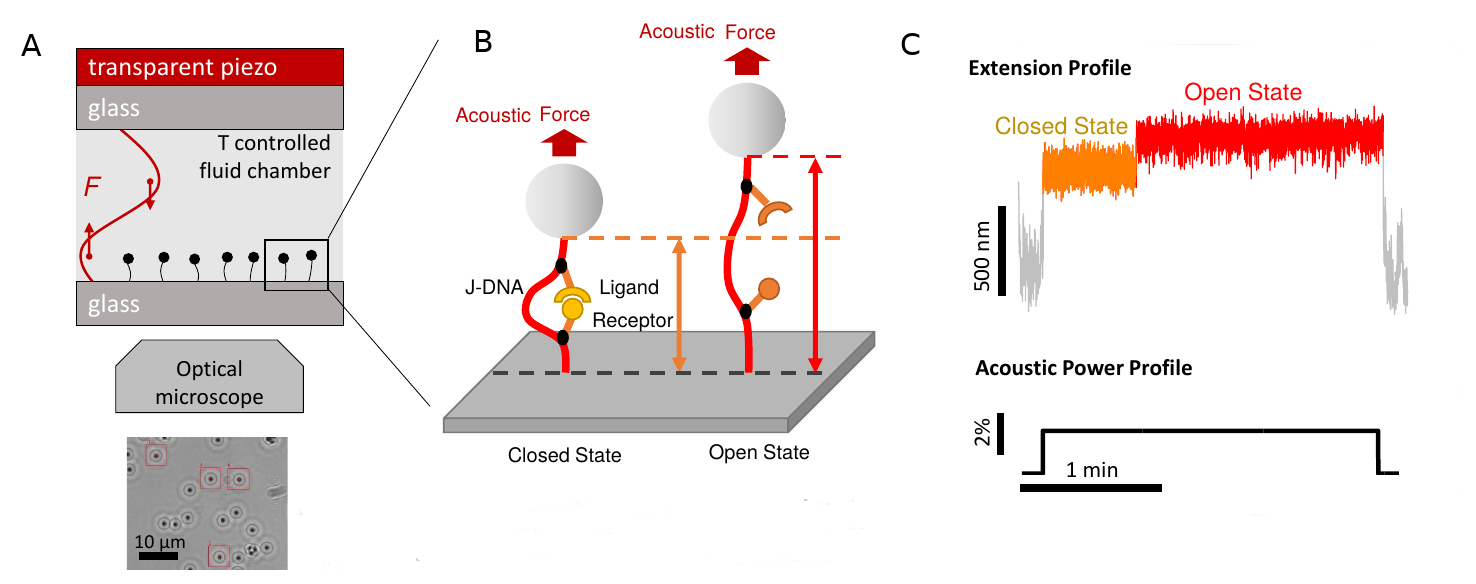
\includegraphics[width=1\linewidth]{Figures/PrincipleAFS-JDNA.png}
	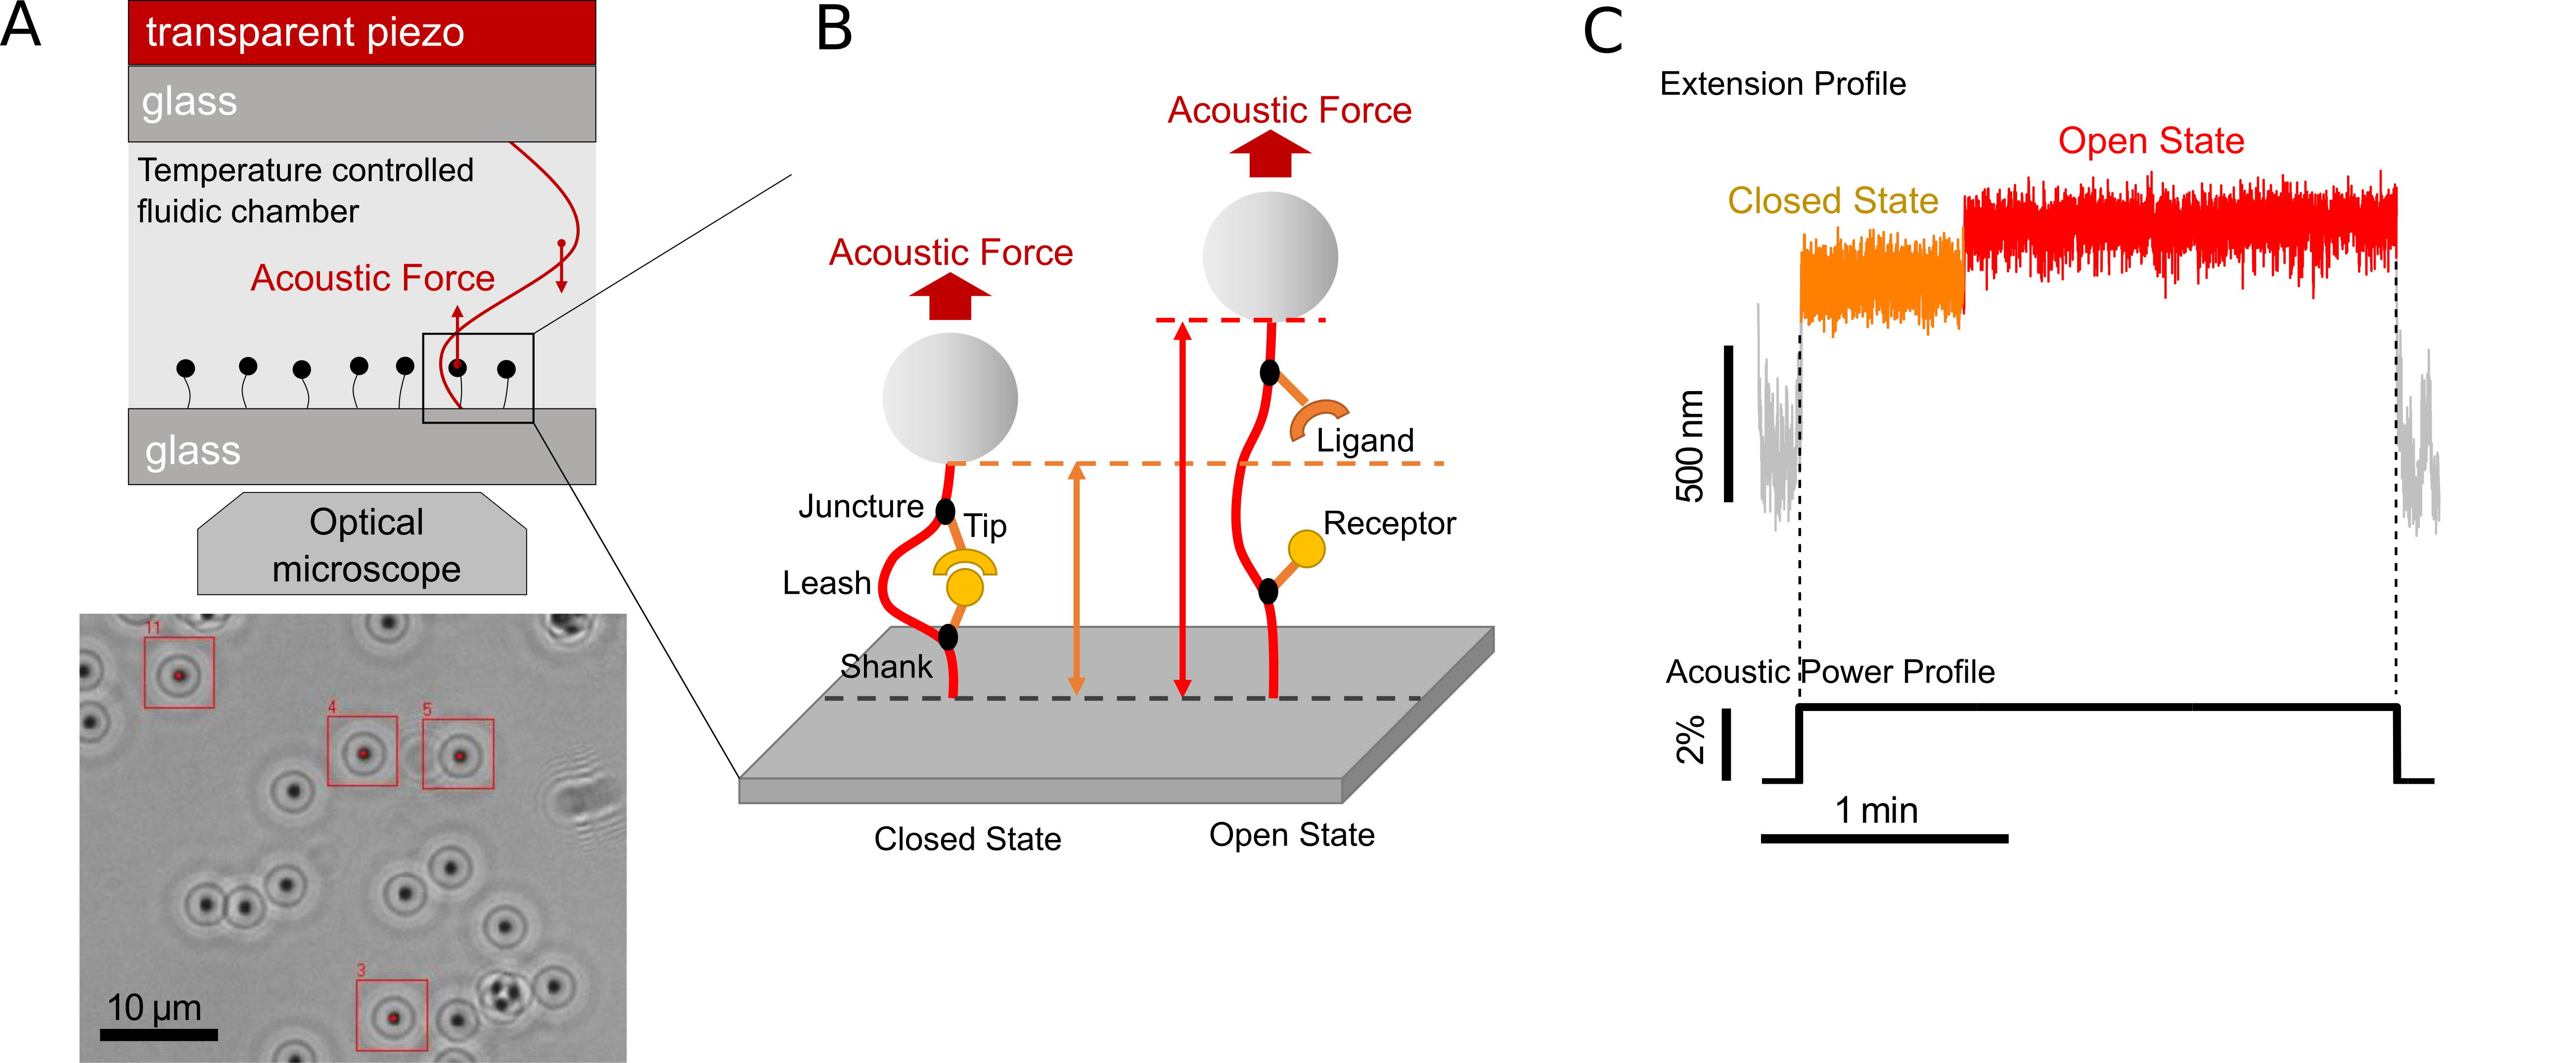
\includegraphics[width=1\linewidth]{Figures/fig1.png}
	\caption{Principle of the method and sample trace. (A) Beads are placed in a microfluidic chamber equipped with a piezo element and temperature control. Microscopic images of beads are tracked in real-time and 3D based on fringes of diffration. (B) The beads are tethered to the chamber surface through a J-DNA scaffold maintaining the protein partners via a leash. Upon application of acoustic force, the extension of the scaffold in close and open state allows to distinguish the unbinding of the protein complex, as illustrated on the trace of the vertical position of the bead in (C).}
	%		 (B) The J-DNA is immobilized at two ends (chamber surface and microbead), while ligand and receptor are maintained on the scaffold via a leash. Upon application of acoustic force, the close and open state of the ligand-receptor complex are distinguished via the scaffold extension, as illustrated on the trace of the vertical position of the bead in C.}
	\label{fig:principle}
\end{figure}


%As described in the Materials and Methods, the J-DNA scaffolds are pre-assembled with FKBP12 and FRB in the absence of Rapamycin, before injection in the AFS chamber. The AFS chamber floor is coated with Anti-Dig for J-DNA binding and BSA for passivation. J-DNA are injected into the chamber and bind via their Dig residues to the Anti-Dig surface. Next step consists in the injection of streptavidin coated microbeads, which bind to the J-DNA biotin residues. A slow rinsing permit to evacuate the non attached beads from the chamber. Then Rapamycin is injected and mediates the formation of the FKBP12-Rapamycin-FRB complex.
%The application of an alternative tension in the MHz frequency range to the transparent piezoelectric element creates a stationary acoustic pressure field in the chamber. The resonance frequency, as pre-calibrated for each AFS chamber by the manufacturer, is chosen to maximize the vertical pressure gradient at the vicinity of the floor chamber. Two pressure nodes are located typically at 25 $\mu$m and 75 $\mu$m altitude in the 100 $\mu$m high chamber internal space. The driving tension amplitude is scaled as a ‘power’, expressed in \%, designed to scale linearly with the force applied to a bead at a given altitude in the chamber. The AFS chamber is placed on an inverted microscope equipped with a 20x objective and transmitted light.
 
The principle of the method is schematically described on Fig. \ref{fig:principle}A, B. After bead injection in the chamber, the application of a limited acoustic power (1\%) permits to collect non tethered beads at the first pressure node, far out of focus, and to identify the beads tethered to the surface via the J-DNA. This subset of tethered beads is selected to be tracked using the acquisition software. Additional bead sorting can be performed by eliminating the beads for which the recorded x/y trace is strongly anisotropic, which is a typical feature of beads tethered via multiple tethers. If available in the field of view, one or several beads showing no brownian motion can be selected as reference beads to correct baseline drift. The calibration along the optical axis (z direction) is then performed by moving the microscope stage in the z direction on a definite range and recording the diffraction pattern (see Fig \ref{fig:principle}A) of all labeled beads \cite{gosse2002, sitters2015}. 

Fig. \ref{fig:principle}C shows the typical z trace during one force cycle. At low force, it exhibits strong z fluctuations (Fig. \ref{fig:principle}C, first part of the grey trace). Upon application of a 2\% acoustic power, the z value increases quickly to a plateau value and exhibits reduced fluctuations, corresponding to the close state of the scaffold with bound FKBP12-Rapamycin-FRB complex (Fig. \ref{fig:principle}C, orange trace). A sharp transition to a higher plateau is observed, corresponding to the open state, where the FKBP12-Rapamycin-FRB complex is dissociated (Fig. \ref{fig:principle}C, red trace). The difference in z value between the two plateaus corresponds to approximately 200 nm, as expected from the length of the leash in the J-DNA scaffold (Table S2). The power is turned back to a low value to start a new cycle, releasing the tension on the leash and permitting rebinding of the complex (Fig. \ref{fig:principle}C, last part of the grey trace).

The analysis starts with correcting the baseline of x,y,z traces using reference beads or self-reference (see Materials and Methods for details). Anchor point is determined from part of the trace at low power preceeding the force cycle. From the cycle part of the trace, automatic step detection permits to : 1) measure the duration in closed state (bound complex) under application of high power 2) distinguish the open and close states on the trace at test power. An example of z trace obtained during 100 low/high power cycles is shown on Fig. \ref{fig:lifetime}.

\begin{figure}[hbt!]
	\centering
%	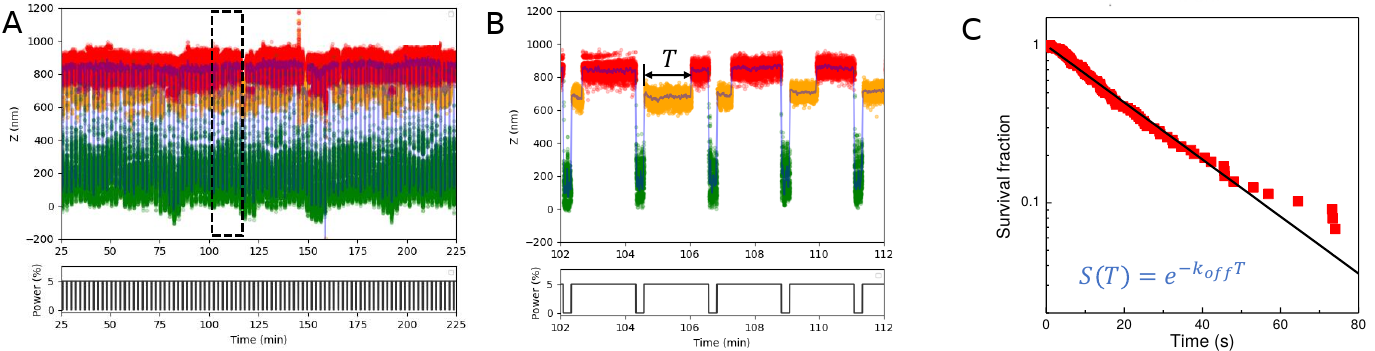
\includegraphics[width=1\linewidth]{Figures/LifetimeMeasurement.png}		
	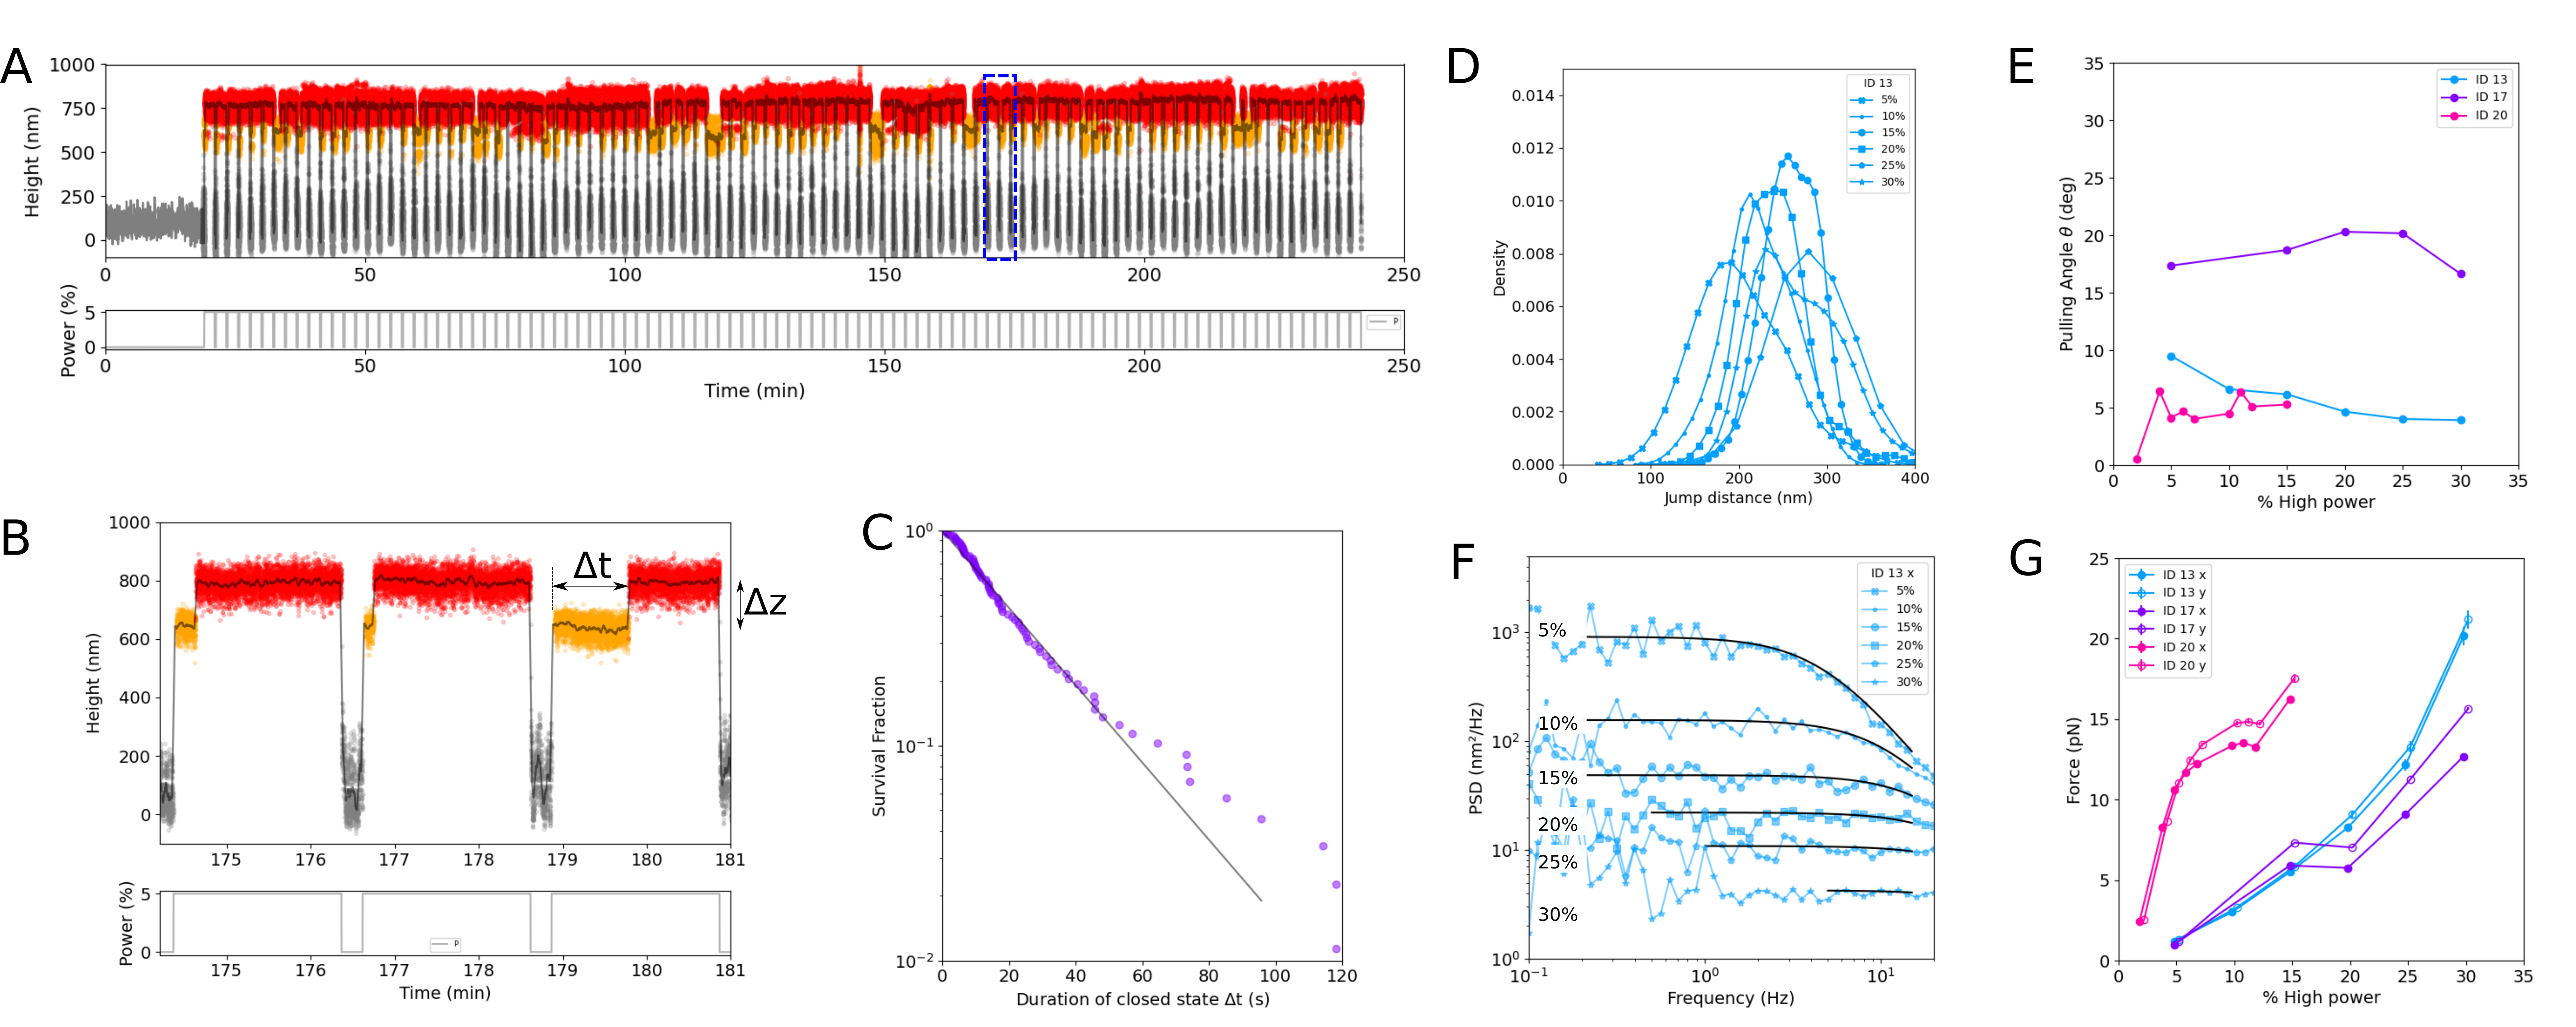
\includegraphics[width=0.75\linewidth]{Figures/fig2.png}
	\caption{ Tracking of a single bead under force cycles and bond lifetime determination. (A) Vertical trace Z obtained during 100 alternate low/high power cycles. (B) Zoom of trace in A. Based on power value and jump detection at high power, the trace is divided in 3 subsets: low power (green), closed state under force (orange), open state under force (red). The lifetime $\Delta$t of the bond corresponds to the duration of the blue step. (C) Corresponding survival curve represented in semi-log scale with superimposed mono-exponential fit : $S(t) = \exp(\Delta t. k_{{\rm off}})$. (D, E) Power Spectrum Density for two representative beads at various applied power. Curves fitted to determine bead radius $R$ and stiffness $k_i$ are shown as black lines. (F) Force vs acoustic power for 3 representative beads. Plain symbols from x direction. Empty symbols from y direction. (G) Pulling angle vs acoustic power for 3 representative beads.}
	\label{fig:lifetime}
\end{figure}


\subsection*{Pulling angle and tether length}
The pulling angle $\theta$ is determined as the angle formed between the optical axis and the segment formed by the anchor point and the bead center in the J-DNA open conformation, (see Eq. \ref{eq:AngleTheta}). Figure \ref{fig:MultiAngle} shows the values we measured for 21 beads tethered by J-DNA functionalized with FKBP12 and FRB, the applied acoustic power being tuned between 2 and 30 \%. In the same field of view the average pulling angle varies between 0 and 60$^{\circ}$ from bead to bead. More strikingly, although $\theta$ is independent of $P^H$ for most of the scaffolds, it may somtimes increase or decrease continuously over nearly 50$^{\circ}$ in the explored power range (see ID 1, 5, 19 for instance ). This is illustrates the existence of lateral pressure nodes which orient the pulling axis and whose position can vary with power.

The length of the J-DNA is measured between the anchor point on the chamber surface and the attachment point to the bead, as illlustrated by Fig. \ref{fig:Lengthcalculation}, following Eq. \ref{eq:Length}.

% and the bead center, minus the bead radius following Eq. \ref{eq:Length}. %We observe that in the range of applied power, the length is monotonically increasing (Fig. \ref{fig:MultiLength}). Also, we observe that the length can exceed the nominal length (ID 12).

\subsection*{Force calibration}
The force calibration is performed by recording the lateral fluctuations of each bead and computing the power spectra density for x and y coordinates. The PSDs of 21 beads  tethered by J-DNA functionalized with the FKBP12-Rapamycin-FRB complex are shown on Fig \ref{fig:FitSpectra}. For each bead, the x or y PSD are fitted together for all powers using Eq. \ref{eq:PSD} with one single bead radius $R_b$, and one value per power for the stiffness $k_i$. The fits are superimposed to the data on Fig. \ref{fig:FitSpectra}, showing a good agreement for all powers. Spectra for 9 beads functionalized with the Nef-Nef19 complex are shown on Fig. \ref{fig:FitSpectraNef}, showing also a good quality of the fit.
For the rapamycin complex, Fig. \ref{fig:PowerStiffness} shows the fitted stiffnesses for each molecule and power. The stiffnesses measured in x or y directions exhibit very similar values. Remarquably, the stiffness varies non-linearly with power, and can exhibit a concave or convex form, illustrating the variability of the stiffness vs power relation.
%The diffusion coefficient for all power is comparable with values obtained applying independent fits for low power (see Fig. \ref{fig:PowerDiffusion}). The difference in x and y direction does not exceed 10\%. The distribution of bead radius obtained from the fit is shown on Fig. \ref{fig:Rdiffusion}

The force is then calculated following Eq. \ref{eq:Force}. The dependence of force with applied acoustic power exhibit the non-linear behaviour similar to the one observed for the stiffness (data not shown). % on Fig. \ref{fig:PowerForce} and.
The force typically varies in the 0-20 pN range, with maximum varying significantly between different positions in the chamber, illustrating the spatial dependence of the technique \cite{nguyen2021}.


\subsection*{Force dependence of open J-DNA length}

The variation of length of open J-DNA as a function of applied force is shown for several molecules in Fig. \ref{fig:ForceLength}. It follows roughly a worm-like-chain (WLC) model, as shown by the superimposed fit in Fig. \ref{fig:ForceLength}. Fig. \ref{fig:Lp_vs_L0} shows the distribution of the persistence length and contour length. This shows a dispersion between typically 1000 and 1700 nm for the contour length, and between 5 and 10 nm for the persistence length. We attribute this variability and the negative correlation (-0.5) to the limited number of points in the WLC fit. Nevertheless, the J-DNA scaffold appears quite flexible compared to its ds-DNA constituents, probably due to the strong contribution of the two hinges in the global mechanical response of the scaffold.\\
{\color{red} Accuracy of length measurements and delta z}

\subsection*{Force dependence of off-rate}

The use of J-DNA scaffold allows repetitive measurements on individual bonds.
The fraction of non-closing events remain usually less than 0.2,  %(Fig. \ref{fig:MultiNoClose}),
indicating that the duration at low force is sufficient for an efficient rebinding. It was also noticed that, in case of beads of 1.56 $\mu$m diameter, the cloud of points at low force exhibits a symmetric and homogeneous distribution around the anchor point, facilitating the scaffold recoiling and encounter of the reactive partners. The use of J-DNA also allows to easily measure the bond lifetime under force (Fig2B). The lifetime
corresponds to the duration of the close state, when a jump is detected. %, the lifetime of FKBP12-Rapamycin-FRB complex under applied force is measured (Fig. \ref{fig:lifetime}B).
The lifetimes measured over each force cycle are pooled in a survival curve, which is established for each molecule and applied force (Fig. \ref{fig:MultiSurvival}). Survival curves, as represented in a semilog plot, are individually fitted by a single mono-exponential function, which slope represents the off-rate (Fig. \ref{fig:lifetime}C). Off-rates are then plotted as a function of force for each molecule and represented in Fig. \ref{fig:offrate_force}. Each one is fitted separately with the Bell function which relates off-rate $ k_{\rm off}$ and applied force $f$ through:

\begin{equation}
\label{eq:Bell}
k_{\rm off} = k^0_{\rm off} \exp \left(\frac{x_b f}{k_B T}\right)
\end{equation}

\noindent where $k^0_{\rm off}$ is the off-rate in absence of applied force and $x_b$ is the distance from the potentiel well to the barrier in the energy landscape of the interaction.

\begin{figure}[hbt!]
	\centering
	\centering
	\begin{tabular}{ccc}
		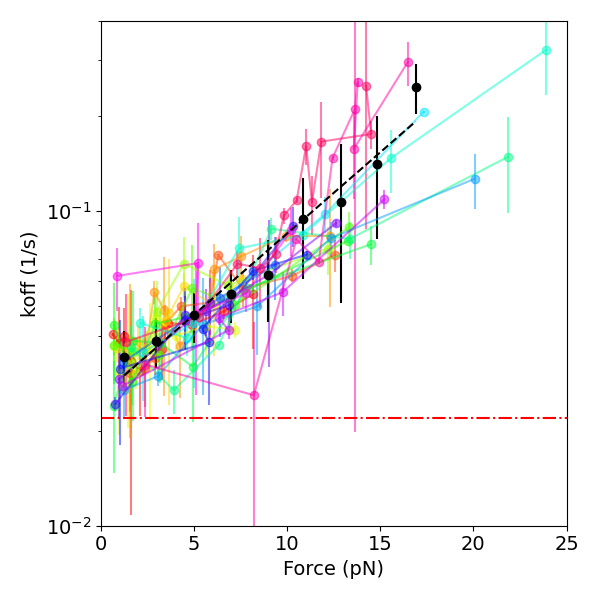
\includegraphics[width=0.45\linewidth]{Figures/offrate_vs_force_Rapa.png} & &	
		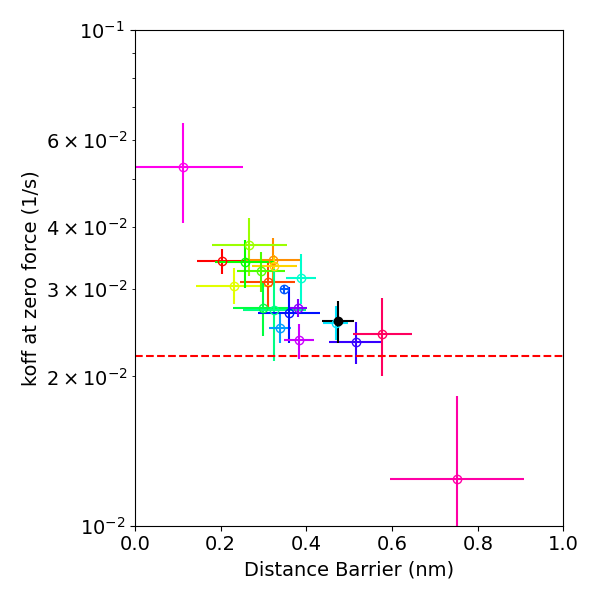
\includegraphics[width=0.45\linewidth]{Figures/koff0_vs_xBeta_Rapa.png}		 \\
	\end{tabular}
	\caption{Off-rate data for FKBP12-Rapamycin-FRB complex and Bell fit. A. The off-rate at different forces of individual molecules is shown in different colors. The average values on force bins of equal size are shown as black disks. The dashed black line is the fit with Bell equation \ref{eq:Bell}. B. Off-rate in absence of applied force $k^0_{\rm off}$ as a function of $x_b$, the distance from the potentiel well to the barrier in the energy landscape of the interaction. The horizontal dashed lines in A and B represent the value of off-rate measured by Surface Plasmon Resonance \cite{banaszynski2005}.}
	\label{fig:bell_parameters}	
\end{figure}

Fig. \ref{fig:bell_parameters}A shows, on the same graph for direct comparison, off-rate vs force plots for 21 J-DNA scaffolds functionalized with FKBP12-Rapamycin-FRB complex. All $ k_{\rm off}$ values are also pooled by force bins (Fig. \ref{fig:bell_parameters}A, black disks) and fitted using Bell equation giving: $k^0_{\rm off}=0.026 \pm 0.002$  s$^{-1}$ and $x_b = 0.47 \pm 0.04$ nm. This is in close agreement with the values retrieved using magnetic tweezers: $k^0_{\rm off}=0.04$ s$^{-1}$ and $x_b=0.42$ nm \cite{kostrz2019}.
{\color{red}Charlie please check MT values }\\
Fig. \ref{fig:bell_parameters}B shows the Bell parameters in the $k^0_{\rm off}$ vs $x_b$ plane, with each colored circle representing the fit from an individual complex, as reported on Fig. \ref{fig:offrate_force}. The black dot corresponds to the values obtained by fitting the pool data represented in Fig. \ref{fig:bell_parameters}A. Off-rates measured at zero force are also consistent with Surface Plasmon Resonance determination of 2.2 10$^{-2}$ s$^{-1}$ \cite{banaszynski2005}, as indicated by the red dashed line in Fig. \ref{fig:bell_parameters}A, B. 

The same measurements and analyses were performed for 9 J-DNA scaffolds functionalized with Nef and Nef19. This complex being much more long-lived than FKBP12-Rapamycin-FRB, we used larger beads (3$\mu$m diameter), in order to increase the acoustic force at equal power, and therefore decrease the bond lifetime, without generating too much heat or shifting the resonance too strongly. Force dependence on applied voltage are represented on Fig \ref{fig:PowerForce_Nef}. A sharp force increase can be observed for beads of 3 $\mu$m diameter, compared to beads of 1.58 $\mu$m diameter. The survival curves are displayed on Fig. \ref{fig:MultiSurvival_Nef}. Despite the force increase, the bond lifetime often exceed the measurement time. Thus, survival curve contain a limited number of rupture events and are censored at a maximal duration between 600 and 1200 s. While independent curves fit of off-rate vs force is not accurate, one can perform the fit on binned data, as shown on Fig. \ref{fig:bell_parameters_Nef}. The Bell parameters are as follows:  $k^0_{\rm off}=0.14 \pm 0.05$  $10^{-3}$  s$^{-1}$ and $x_b = 0.75 \pm 0.08$ nm. As for FKBP12-Rapamycin-FRB, there is an excellent match with off-rate of 1.8 10$^{-4}$ s$^{-1}$ determined in the absence of force \cite{bouchet2011}, indicated as red dashed line on Fig. \ref{fig:bell_parameters_Nef}.
 
\begin{figure}[hbt!]
	\centering
		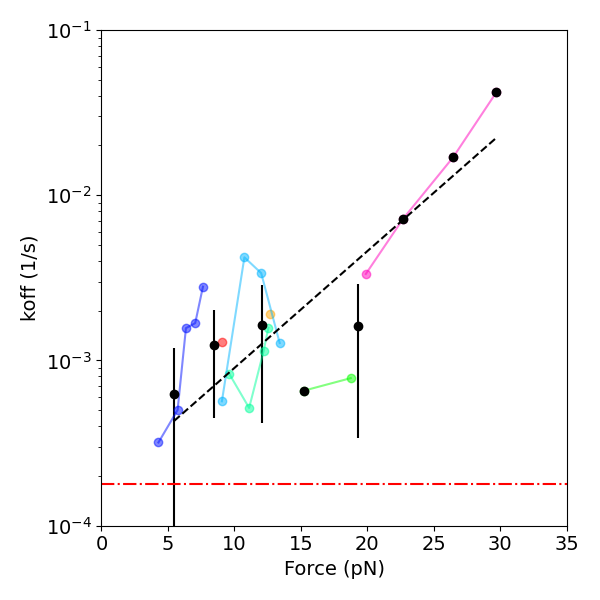
\includegraphics[width=0.4\linewidth]{Figures/offrate_vs_force_Nef.png}	
%	\begin{tabular}{ccc}
%	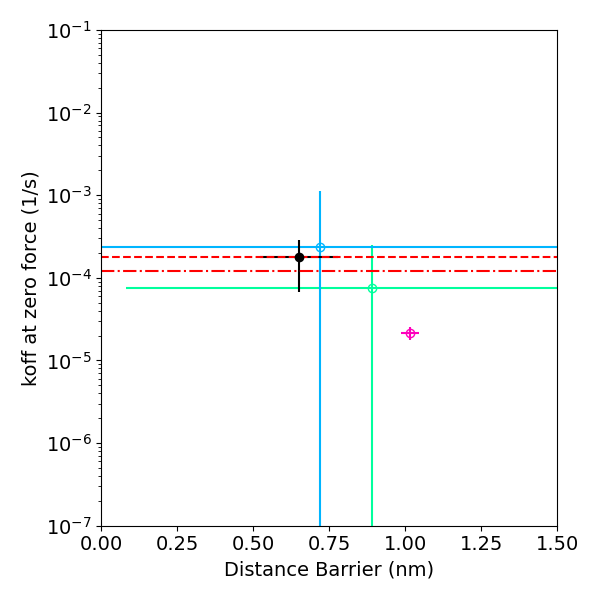
\includegraphics[width=0.4\linewidth]{Figures/koff0_vs_xBeta_Nef.png}		 \\
%	\end{tabular}
	\caption{Pooled off-rate data for Nef-Nef19 complex and Bell fit. The black points are averaged $k_{\rm off}$ by equal force bins. The dashed black line is the fit with Bell equation \ref{eq:Bell}. The horizontal dashed line represents the value of off-rate measured by Surface Plasmon Resonance \cite{bouchet2011}.} %B. Off-rate in absence of applied force $k^0_{\rm off}$ as a function of $x_b$, the distance from the potentiel well to the barrier in the energy landscape of the interaction. The horizontal dashed lines in A and B represent the value of off-rate measured by Surface Plasmon Resonance.}
	\label{fig:bell_parameters_Nef}	
\end{figure}

\subsection*{Accuracy of measurements and robustness of the bond}

Examination of Fig. \ref{fig:bell_parameters}B shows a negative correlation between $k^0_{\rm off}$ and $x_b$ for the FKBP12-Rapamycin-FRB complex. To assess whether it could have a molecular origin, we hypothesized that the elasticity of the scaffold could play a role in this observation \cite{walton2008}. However, we observe no correlation between the $x_b$ parameter, and the mechanical parameters of the scaffold, length and persistence length (data not shown). Additionally, we computed the potential effect of a parabolic potential, as proposed in \cite{friddle2012}. The quadratic term induces a negligeable increase of $k^0_{\rm off}$ for the highest $x_b$ measured. As an alternative interpretation, we propose that the error in fitting the slope in the $k_{\rm off}$ vs force plots leads to a correlated error in the intercept of the y axis. This type of error is possibly explaining spurious correlation identified in early works \cite{schwesinger2000}. Nethertheless, most of the points in Fig. \ref{fig:bell_parameters}B lie on a line, emphasizing the robustness of rupture characteristics among 21 molecules. This is thus questioning the concept of bond heterogeneity \cite{raible2006} as it could be a consequence of measurement inaccuracy. In case of high affinity antibodies with long lifetime, the stability of the setup as well as the precision of force calibration are crucial elements to control in order to adress such issues.

Another advantage of the present technique is the possibility to follow the same molecules over time during cyclic force application, thus probing bond aging. As an example, we compute the off-rate calculated either during the first 50 cycles of a measurements (early off-rate), or during the last 50 cycles (late off-rate). Fig. \ref{fig:maturation} shows that these two quantities are in average identical for the collection of 21 scaffolds functionalized FKBP12-Rapamycin-FRB and subjected to 1-20 pN unbinding forces. Thus, on the time scale of several hours, and a hundred of loading cycles, these bonds do not exhibit measureable aging. 


%{\color{red} Optional: force projection, fit with Friddle term,  (b)
%
%calibration on the fly (see fig) + comparison 'classical' for k and D
%
%contour approach for anchor point: comparison of length
%
%distribution of radius from diffusion
%
%plots of dz jumps
%
%DNA length vs barrier}


%Influence of time on individual scaffolds (Fig 4). Fig 4: Individual over time: within one sequence of cycle; over several cycles (FOV 1, 2, 3)

%
%You can make lists with automatic numbering \dots
%
%\begin{enumerate}
%\item Like this,
%\item and like this.
%\end{enumerate}
%
%\dots or bullet points \dots
%
%\begin{itemize} 
%\item Like this,
%\item and like this.
%\end{itemize}
%
%\dots or with words and descriptions \dots
%
%\begin{description}
%\item[Word] Definition
%\item[Concept] Explanation
%\item[Idea] Text
%\end{description}
%
%An example quotation:
%
%\begin{quote}
%Lorem ipsum dolor sit amet, consectetur adipiscing elit, sed do eiusmod tempor incididunt ut labore et dolore magna aliqua. Ut enim ad minim veniam, quis nostrud exercitation ullamco laboris nisi ut aliquip ex ea commodo consequat.
%\end{quote}


%\section*{Discussion}


%\LaTeX{} formats citations and references automatically using the bibliography records in your .bib file, which you can edit via the project menu. Use the \verb|\cite| command to insert a citation, like this: \cite{Chen_Nicholson00} Multiple citations can be given as \cite{Stiles_Bartol01,el-Kareh_etal93,Callaghan91}. You can use either BibTeX or biblatex: see the following subsections.
%
%If your manuscript is accepted, the Biophysical production team will re-format the references for publication. \emph{It is not necessary to format the reference list yourself to mirror the final published form.}
%
%\subsection*{Using bibtex} 
%This is the default. Specify your \texttt{.bib} file with \verb|\bibliography{sample}| (the extension is unnecessary) near the end of your manuscript, where you want the references list to appear.
%
%\subsection*{Using biblatex} 
%Pass the \texttt{biblatex} option to the \verb|\documentclass| declaration, then specify your \texttt{.bib} file name in the \emph{preamble}: \verb|\addbibresources{sample.bib}| (the extension is necessary). Write \verb|\printbibliography| near the end of your manuscript where you want the references to appear.

\section*{Conclusion}

The present work shows for the first time the combination of AFS and J-DNA to measure the force dependence of individual biomolecular bonds complexes. While AFS gives potential access to an extended dynamic forcerange compared to other techniques, a drawback resides in strong acoustic field heterogeneity and stability, as minute temperature change affects the acoustic resonance frequency. As for other parallel method like laminar flow chamber and MT, a trade-off between bead size should be found to optimize force range while limiting non-specific adhesion. Another practical constraint reside in the current commercial closed format of the chambers, which renders surface reproducible coating delicate. Once such optimal conditions are found, the method shows a good potential due to the modularity of J-DNA: ease-of-access of AFS commercial setup, direct length measurement, in situ force calibration.

While naturally parallel, the method, using in situ force calibration, has a sufficient accuracy for force-dependent rupture characterization on one single FKBP12-Rapamycin-FRB complex. We also illustrate the potential of the method to compare individual bonds of same nature and bond behaviour under repeated actuation. We finally measure the force-induced antigen-antibody bond rupture, opening the way to systematic chemomechanical characterization of biomedically relevant biomolecular bonds.


%Elements of coclusion\\
%
%- modularity of JDNA
%
%- choice of beads: compromise between absoulte force
%
%- acoustic field: heterogeneity, time dependence, stability
%
%- modified software



\section*{Author Contributions}

LL and CG designed the research. JYW and CV carried out experiments. AA, PC, MF, DK, TS, CG contributed reagents. LV, FR contributed to the acquisition software and experimental setup. JYW, CV and LL analyzed the data. JYW, CV, CG and LL wrote the manuscript. All authors critically revised the manuscript.

\section*{Acknowledgments}

We thank AMIDEX Emergence Innovation ForSelecAntibody, PhysCancer program ComPhysAb, Projet exploratoire région PACA 2017 – AcouLeuco, European Research Council (ERC, grant agreement No. 772257), Human Frontier Science Program (HFSP, grant No. RGP0056/2018), PSL valorisation (MF), Ligue Nationale Contre le Cancer,  Marie Curie Sklodowska action (MSCA-IF, grant agreement 895819), Labex Memolife, INSERM and CNRS for regular support.


% Uncomment if using bibtex (default)
\bibliography{AFS-JDNA_MS}

% Uncomment if using biblatex
% \printbibliography

\newpage

\FloatBarrier

\newpage

\section*{Supplementary Material}

An online supplement to this article can be found by visiting BJ Online at \url{http://www.biophysj.org}.

\subsection*{Development of a single-molecule tethered assay on an acoustic force microscope: towards parallel characterization of individual mechano-chemical behaviours}

\textbf{ Jian Yon Wang et al.}

%\section{Supplementary Figures}

\setcounter{figure}{0}
\makeatletter 
\renewcommand{\thefigure}{S\@arabic\c@figure}
\makeatother
\setcounter{table}{0}
\makeatletter 
\renewcommand{\thetable}{S\@arabic\c@table}
\makeatother

\subsection*{Supplementary Figures}

\begin{table}[hbt!] %S1
	\caption{Geometrical parameters characterizing the various anatomical segments making up the two J-DNAs used in the present study. The asymmetrical scaffold is the one described in Kostrz et al. \cite{kostrz2019}; the symmetrical one has been obtained following the same synthesis protocol except that the sequences of the TS 1 and TS2 oligonucleotides were respectively changed for
		ATATGAGGCTGAGGGCAGCCACTGGTAACAGGATTAGCAGAGCGAGGFATGTAGGCGGTGCTACA-GAG
		and
		TGTAAGAGCTGAGGTCGCAATGGAGTGTCATTCATCAAGGACGCCGCFATCGCAAATGGTGCTATCC (5’ to 3’ direction, F = azido-dT, underlined bases correspond to the Nb.BbvCI nicking site). The extension jumps associated with the detection of a protein-protein interaction were computed by subtracting the length of the scaffold in the closed conformation to the one in the open conformation}
	\label{tbl:s1}
	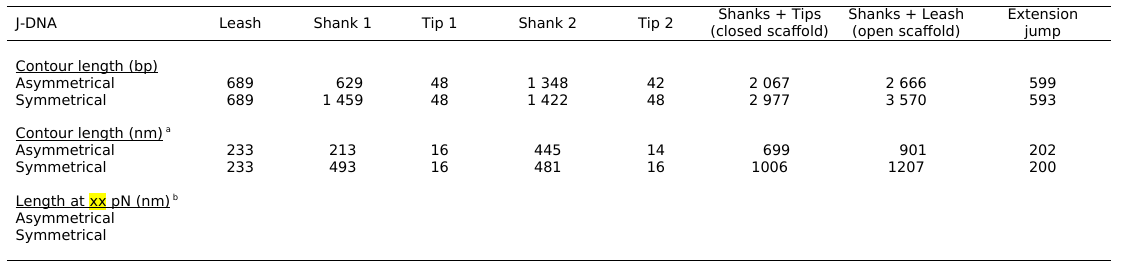
\includegraphics[width=\linewidth]{Figures/TableS1pdf.png}
\end{table}

\noindent
a Calculated assuming a rise of 3.38 Å per base pair \cite{smith1996}.\\
b Calculated using the worm-like chain model with a 50 nm persistence length \cite{bouchiat1999, bustamante1994 }, a value poorly dependent on the ionic strength when it exceeds  20 mM \cite{baumann1997}. 

\begin{table}[hbt!] %S2
	\caption{Geometrical parameters characterizing the different transitions one can observe with the symmetrical J-DNA scaffold. If there is only one high extension state, which identifies with the open conformation, there are five possible low extension states, which correspond to the two tips specifically interacting together, thus yielding the closed conformation, and to one of the tips interacting with one of the surfaces. The contour lengths of the various anatomical segments weres elected so as to associate a unique extension jump value with the detection of a protein-protein interaction; hence, all the other step variations, which are larger, report on non-specific phenomena.}
	\label{tbl:s2}
	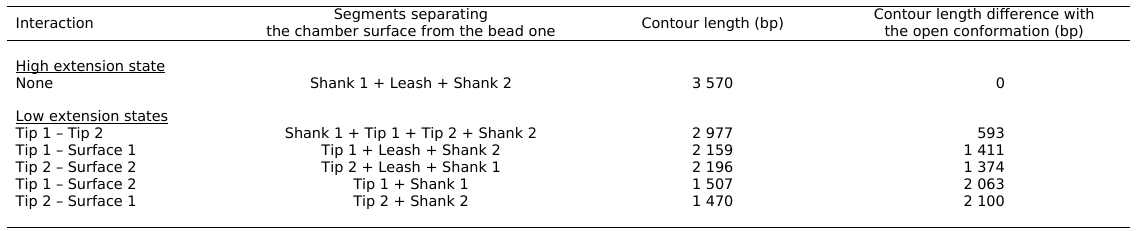
\includegraphics[width=\linewidth]{Figures/TableS2pdf.png}
\end{table}


\begin{table}[hbt!] %S3    %\rightleftarrows
	\caption{Published kinetic parameters for the FKBP12-rapamycin-FRB    FKBP12-rapamycin    FRB reaction.  corresponds to the dissociation equilibrium constant,  to the dissociation rate constant, and  to the association rate constant. a}
	\label{tbl:s3}
	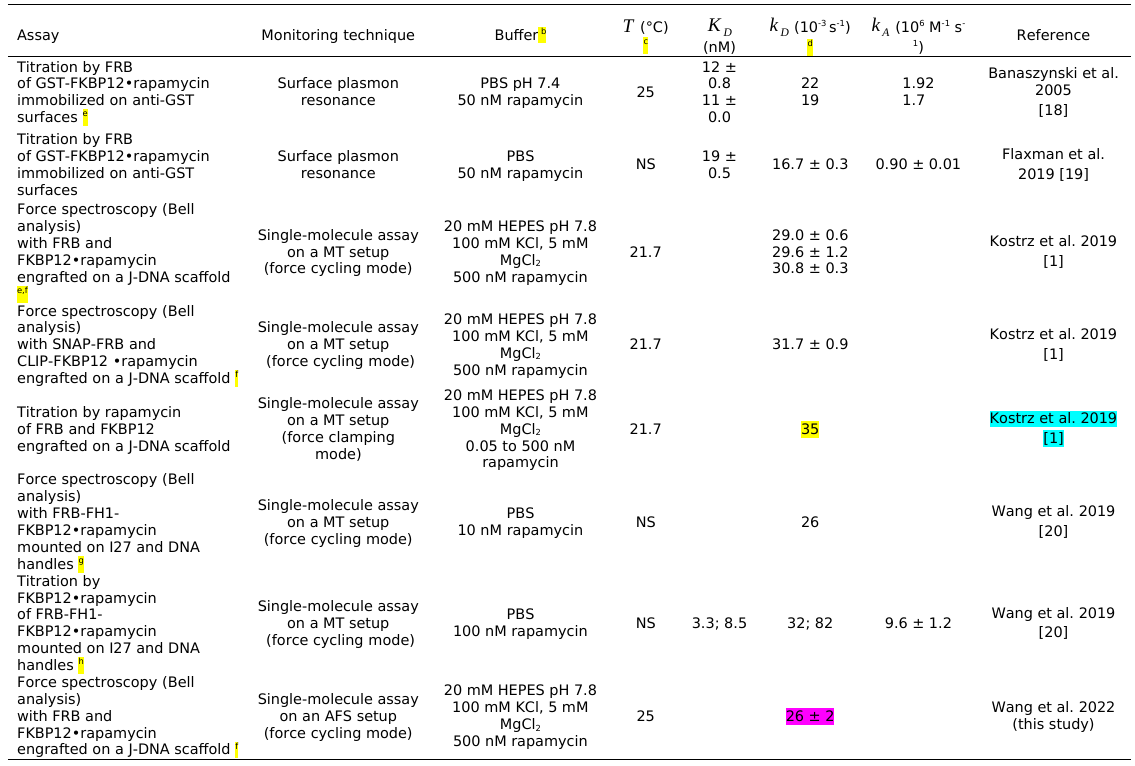
\includegraphics[width=\linewidth]{Figures/TableS3pdf.png}
\end{table}

\noindent
a Abbreviations: GST = glutathione S-transferase; MT = magnetic tweezers; SNAP, CLIP = two self-labelling protein tags that react with small molecules O6-benzylguanine and O6-benzylcytosine, respectively; PBS = phosphate buffer saline; FH1 = an intrinsically disordered peptide derived from the FH1 domain of formin mDia1; I27 = the immunoglobulin-like domain of titin; AFS = acoustic force spectroscopy.\\
b The dissociation equilibrium constants for the FKBP12•rapamycin and FRB•rapamycin complexes have been reported between  0.2 and 2 nM and between  2 and 20 nM, respectively (see the data compiled in Kostrz et al. 2019 [1] and Joshi et al. 2021 paper in print). Therefore, it is assumed that for rapamycin concentrations ranging from 10 to 100 nM FKBP12 is nearly fully occupied by the macrolide whereas FRB is nearly free of it [18,20]: one studies the interaction between FKBP12•rapamycin and FRB.\\
c This parameter is sometimes not specified (NS).\\
d This parameter corresponds to the  obtained in force spectroscopy measurements. Since Kostrz et al. provided , the logarithm of the rate constant at zero-force, we computed  and  [21].   
e Data given for different replicates.\\
f Both FRB and FKBP12 are attached to the scaffold by their N-terminus. Engraftment of the proteins on internal amino acids provides dissociation rate constants at zero force within error bars (see Table S4).\\
g FRB and FKBP12 are attached to their handles by their N- and C-terminus, respectively.
h A biexponential fit yielded two characteristic dissociation times and thus two dissociation rate constants; by combination with the single association rate constant it led to two dissociation equilibrium constants. Only one concentration point, at 1 nM FKBP12, was used in this study.\\

\newpage

\begin{table}[hbt!]  %S4
	\caption{Published kinetic parameters for the FKBP12-rapamycin-FRB    FRB reaction    FRB dissociation. $k_D0$ corresponds to the dissociation rate constant at zero-force and $z_D$ o the distance to the transition state, both obtained from fitting data with the Bell equation}
	\label{tbl:s4}
	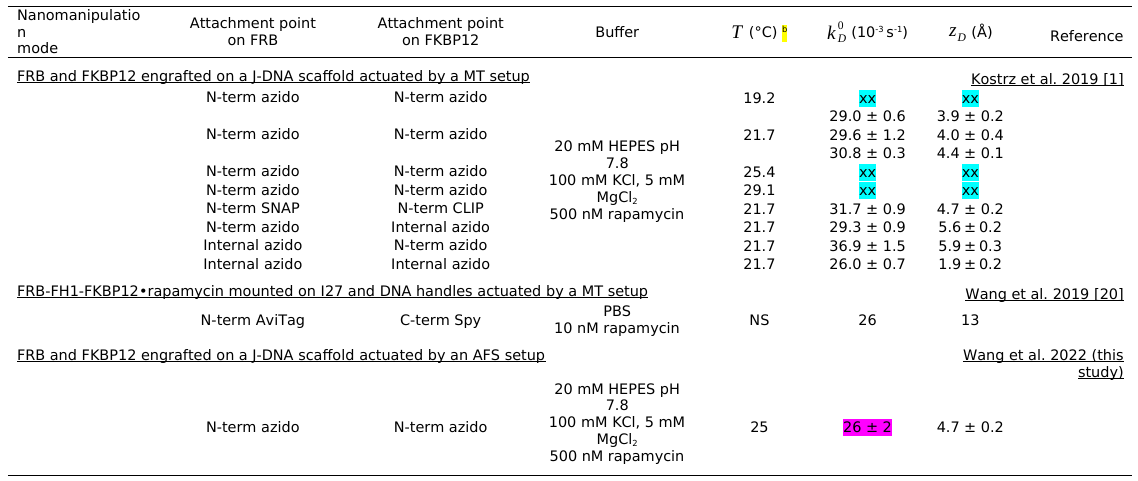
\includegraphics[width=\linewidth]{Figures/TableS4pdf.png}
\end{table}
\noindent
a Abbreviations: MT = magnetic tweezers; azido = clicking to  ; SNAP, CLIP = two self-labelling protein tags that react with small molecules O$^6$-benzylguanine and O$^6$-benzylcytosine, respectively; AviTag = a peptide tag that can be labelled with biotin for further bonding to streptavidin; Spy = a peptide tag that reacts with the SpyCatcher protein; PBS = phosphate buffer saline; FH1 = an intrinsically disordered peptide derived from the FH1 domain of formin mDia1; I27 = the immunoglobulin-like domain of titin; AFS = acoustic force spectroscopy.
b This parameter is sometimes not specified (NS).


\begin{figure}[hbt!]
	\centering
%		\begin{tabular}{ccc}
%		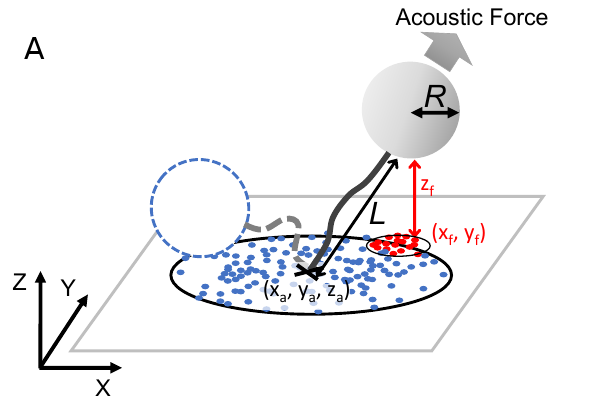
\includegraphics[width=0.35\linewidth]{Figures/LengthCalculation.png} &
%		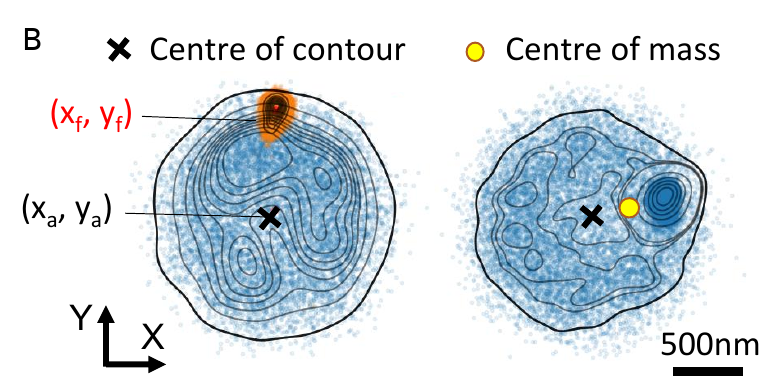
\includegraphics[width=0.35\linewidth]{Figures/AnchorPoint.png} &	
%		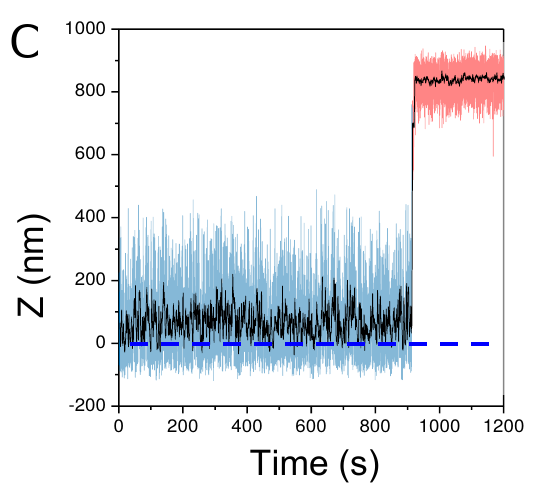
\includegraphics[width=0.2\linewidth]{Figures/AnchorPointZ.png}		 \\
%
%		\end{tabular}

		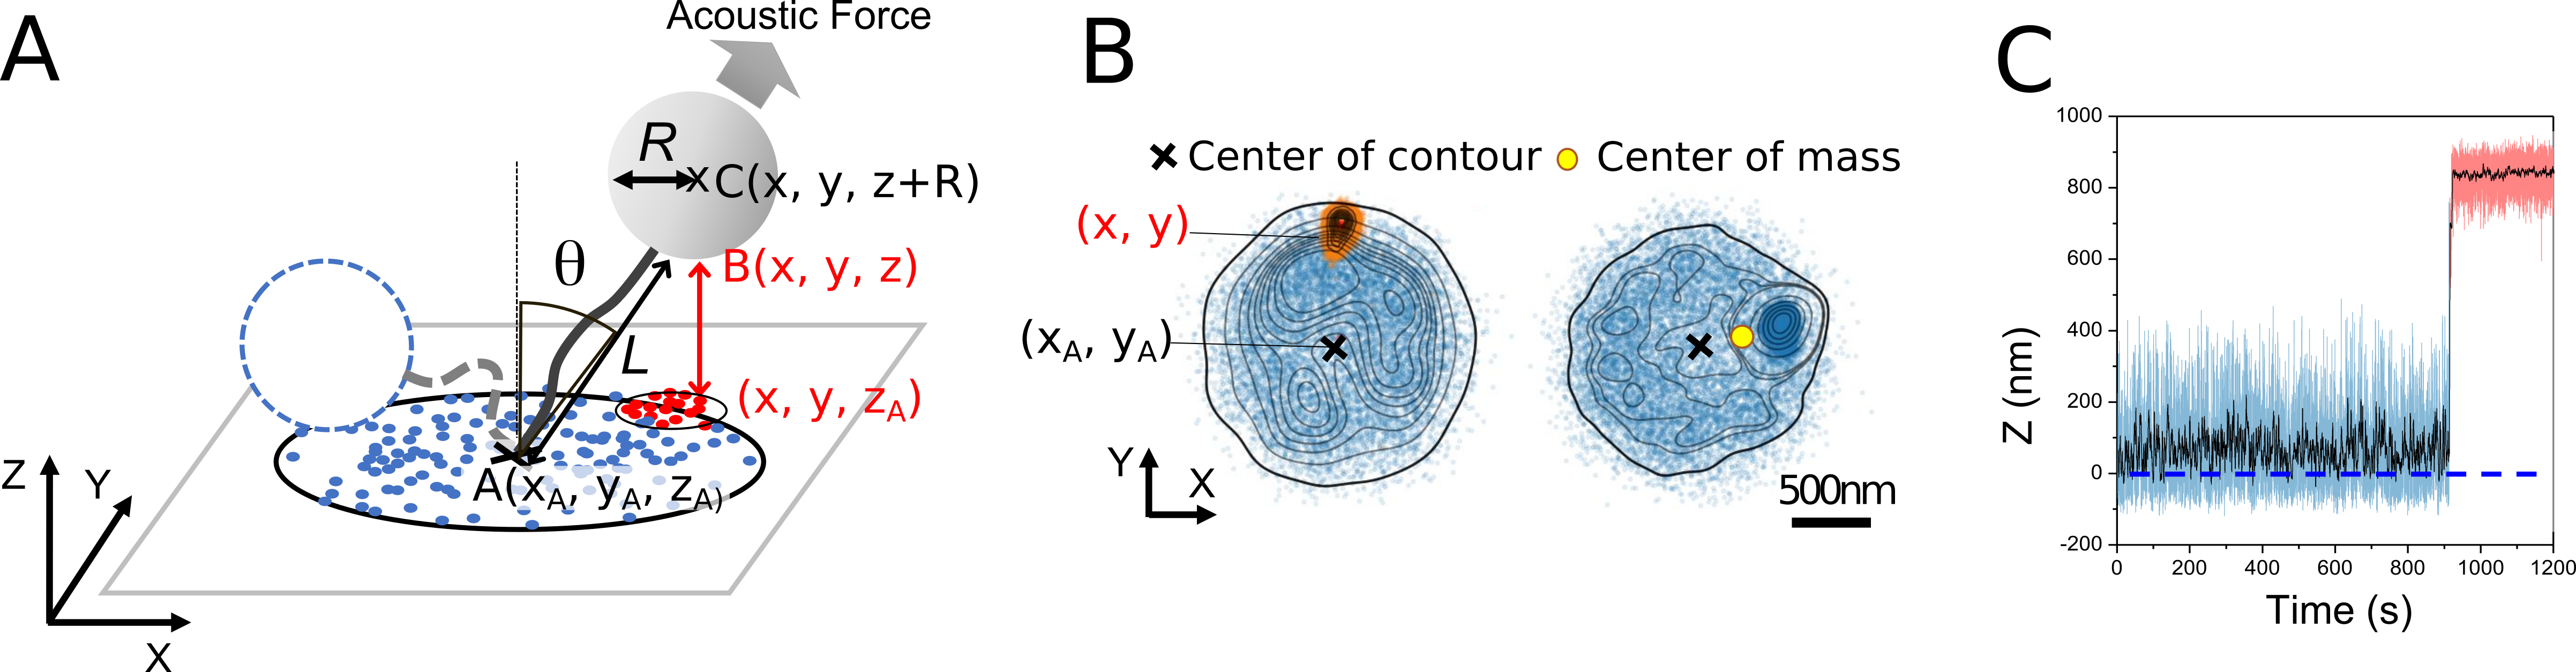
\includegraphics[width=1\linewidth]{Figures/figS1.png}

	\caption{(A) Geometrical notations to determine anchor point A, scaffold length $L$ and pulling angle $\theta$ (see Eqs. \ref{eq:Length} and ref{eq:AngleTheta}). The blue points are the projection of bead position on the (x,y) plane when low or zero force is applied. The red points are the projection of bead positions when an acoustic force is applied. (B) Left: Illustration of the effect of pulling angle $\theta$ on the lateral shift between anchor point A and bead position B at high force. Right: Illustration of the use of a density kernel on lateral positions to determine the anchor point as center of the external density map contour, in case the trace exhibits spurious sticking points. C. Graphical representation of the convention to establish the zero altitude (dashed line) after time average of z trace fluctuations (in black).}
	\label{fig:Lengthcalculation}
\end{figure}

\begin{figure}[hbt!]
	\centering

	\centerline {\includegraphics[width=0.8\linewidth]{Figures/Fig_calibration on the fly.png}}
	\caption{Comparison of power spectra densities for single step vs on the fly calibration}
	\label{fig:Onthefly}	
\end{figure}

\begin{sidewaysfigure}[hbt!]
	\centering
	 \centerline {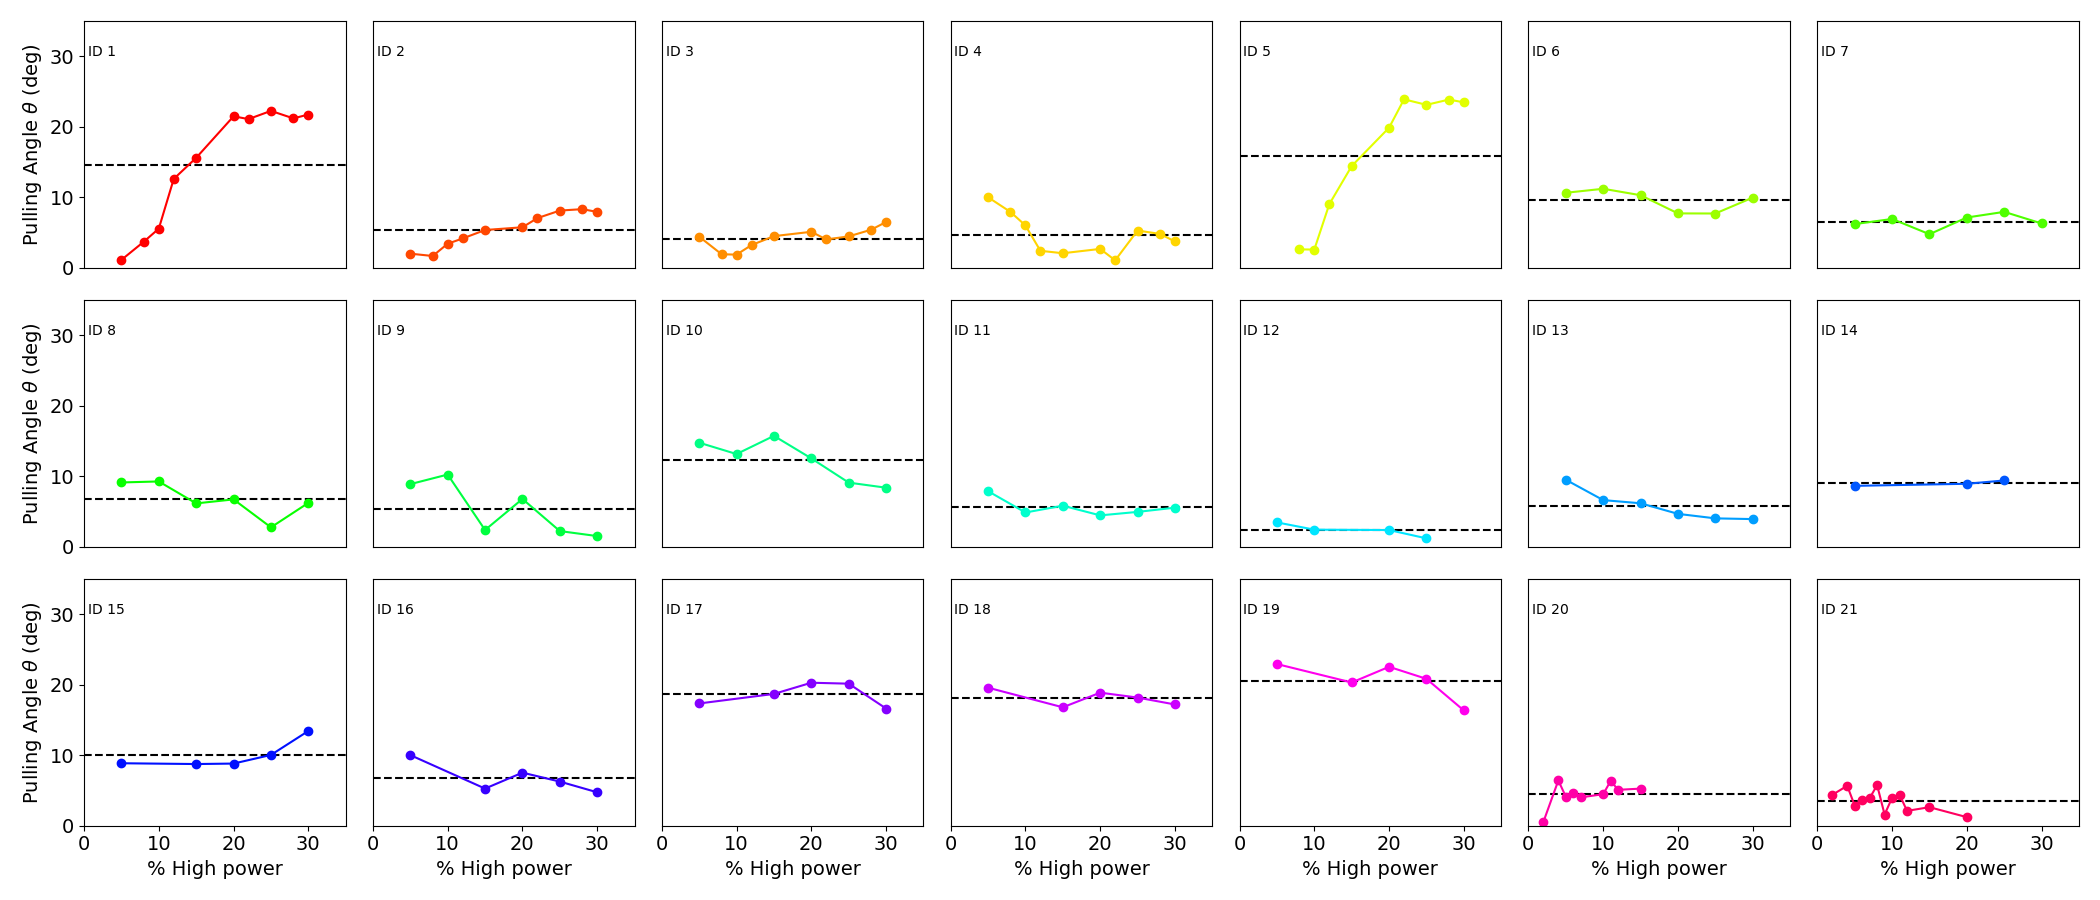
\includegraphics[width=1.0\linewidth]{Figures/Power_Angles_Rapa.png}}
		\caption{Pulling angle $\theta$ as a function of applied acoustic power for 21 beads tethered by J-DNA functionalized with the FKBP12-Rapamycin-FRB complex. Average angle for one bead is indicated as a dashed line.}
	\label{fig:MultiAngle}	
\end{sidewaysfigure}

%\begin{figure}[hbt!]
%	\centering
%	\centerline {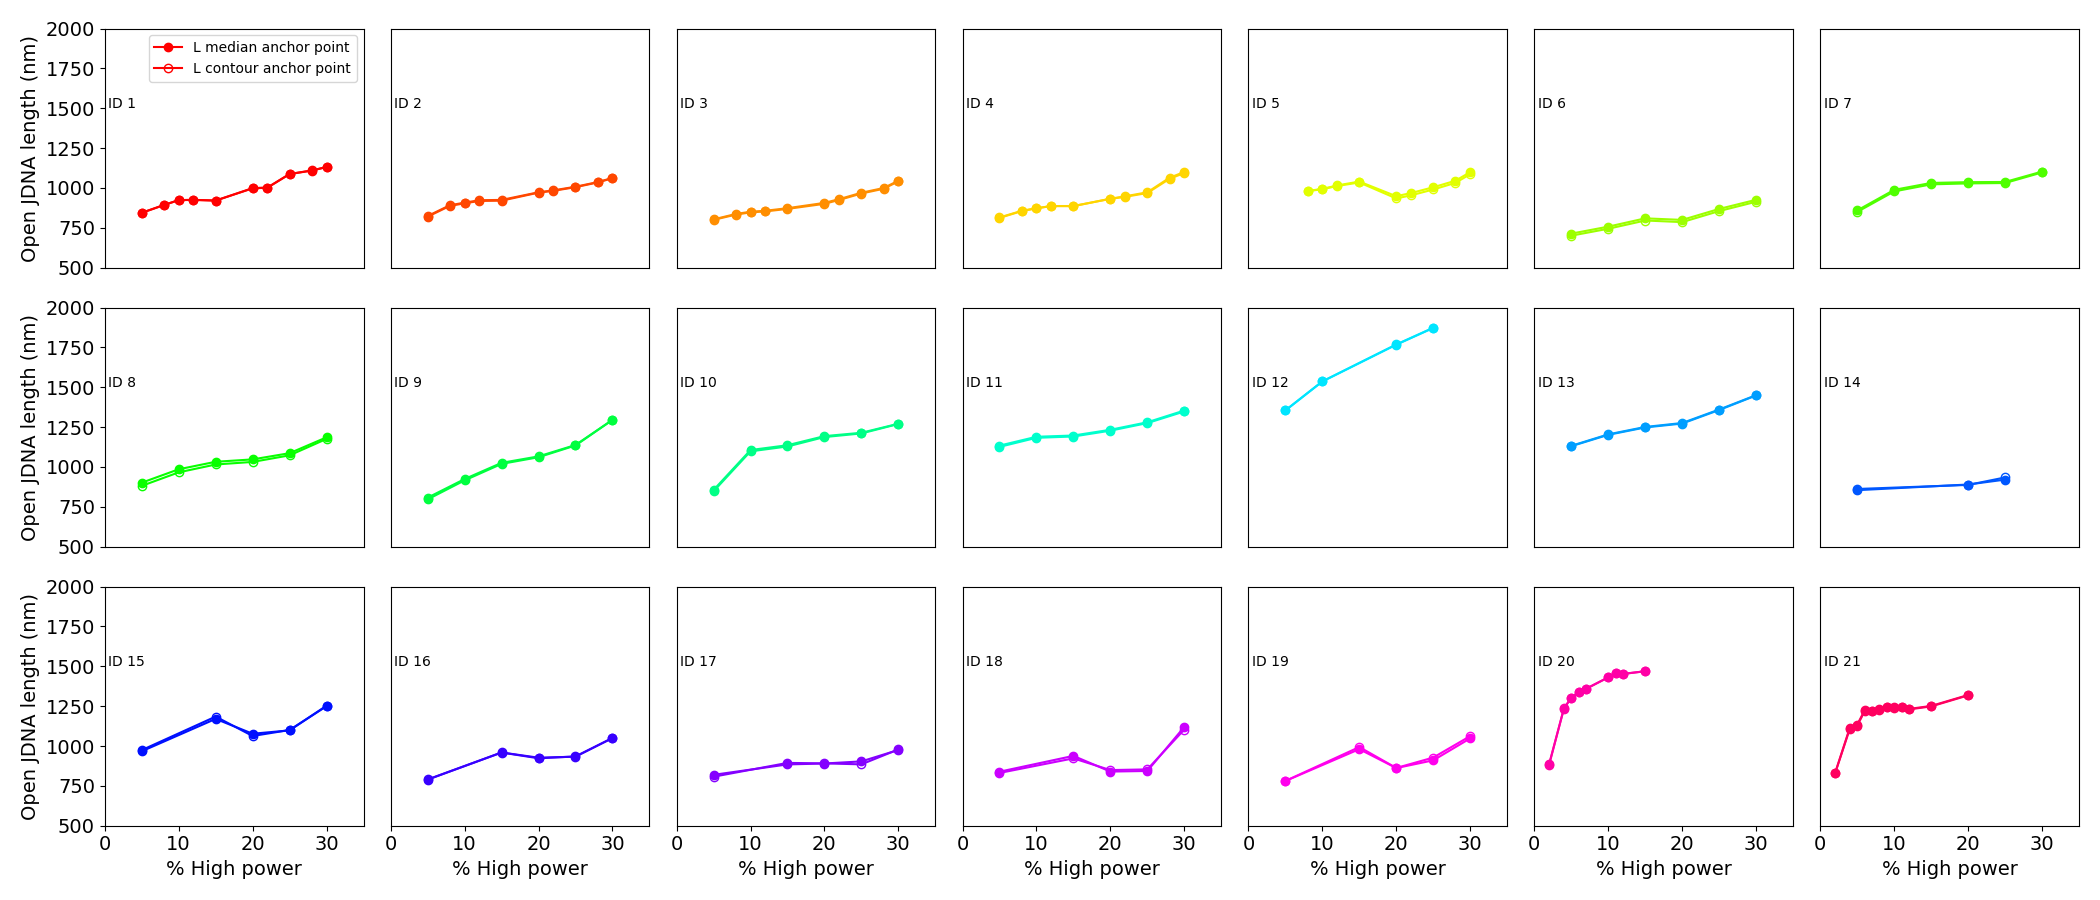
\includegraphics[width=1.2\linewidth]{Figures/Power_Lengths_Rapa.png}}
%	\caption{Open Length (in nm) of J-DNA functionalized with the FKBP12-Rapamycin-FRB complex as a function of applied acoustic power for 21 beads.}
%	\label{fig:MultiLength}	
%\end{figure}

\begin{sidewaysfigure}[hbt!]
	\centering
	\centerline {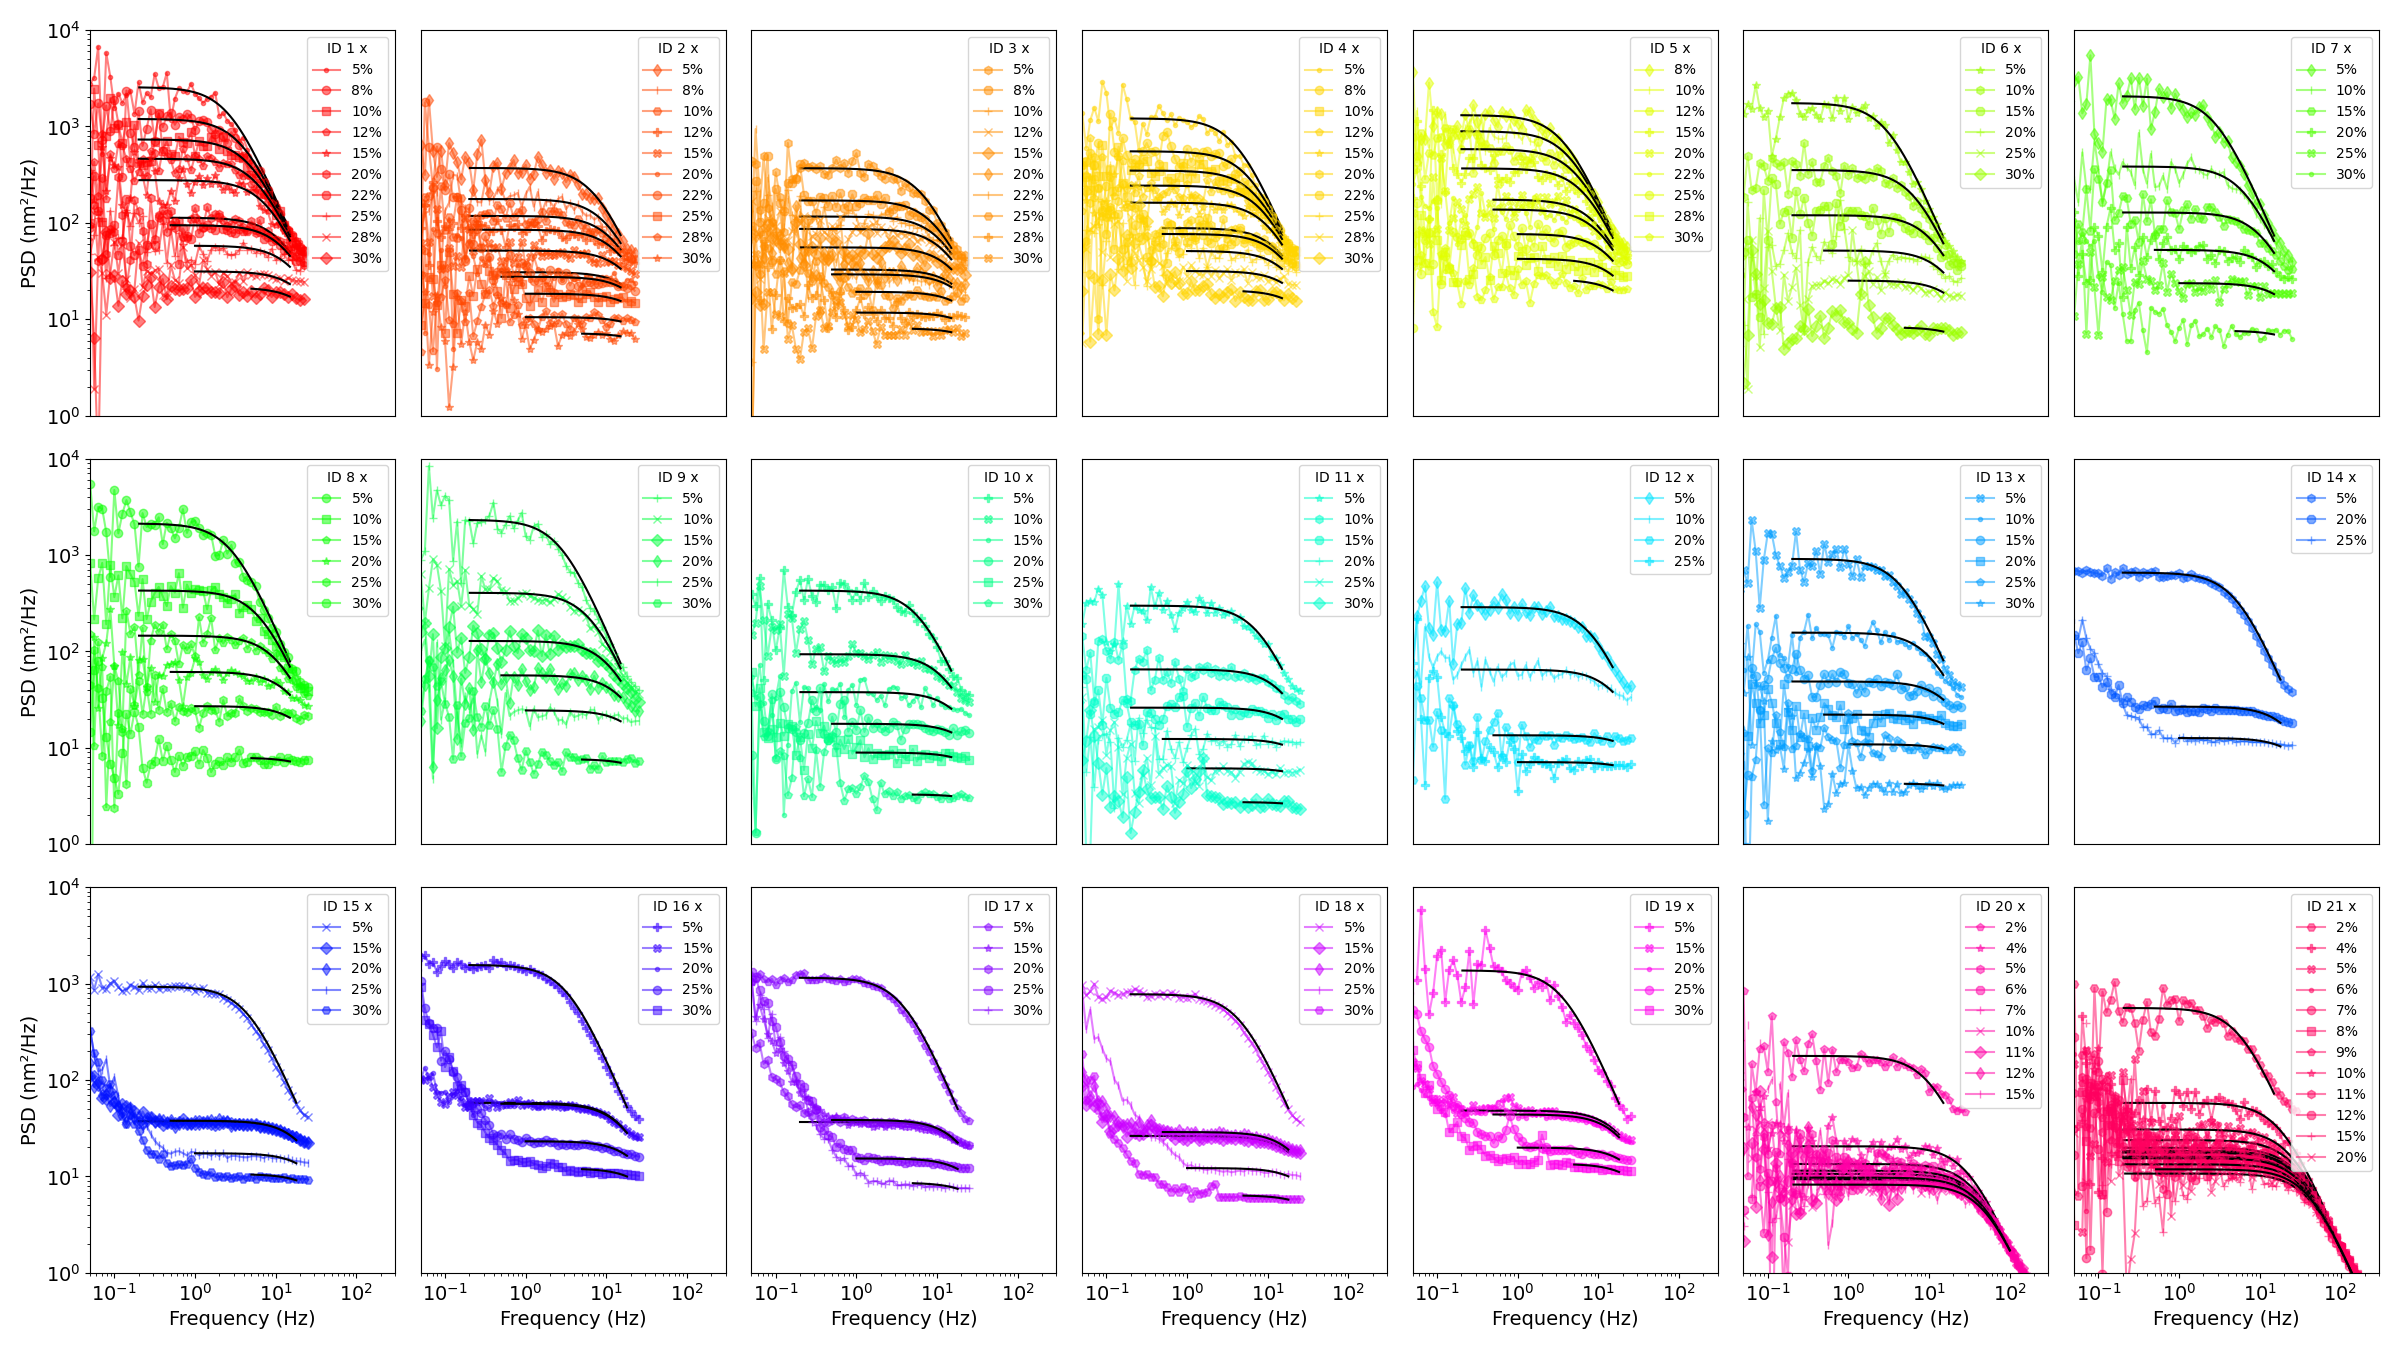
\includegraphics[width=1\linewidth]{Figures/multispectrumx_Rapa.png}}
	\caption{Power Spectra density of x fluctuations for 21 beads tethered by J-DNA functionalized with the FKBP12-Rapamycin-FRB complex and subject to different applied acoustic power. Fits with Eq. \ref{eq:PSD} are superimposed, taking for each bead as fitting parameters : the bead radius $R_b$ and the pendulum stiffness $k_i$ for each power. The fitting range is determined to contain the plateaus of all curves as well as the corner frequency $f_c$, if the condition $f_c < f_{max}/2$ is fullfilled.}
%	{\color{red}Note: ID 14 to 21 (FOV3) spectra have been calculated form cycle mode.
%	All ID correspond to the same experiment, with Maryne's construct; except 35, 36 with Adrien's construct.} }
	\label{fig:FitSpectra}
\end{sidewaysfigure}

\begin{sidewaysfigure}[hbt!]
	\centering
	\centerline {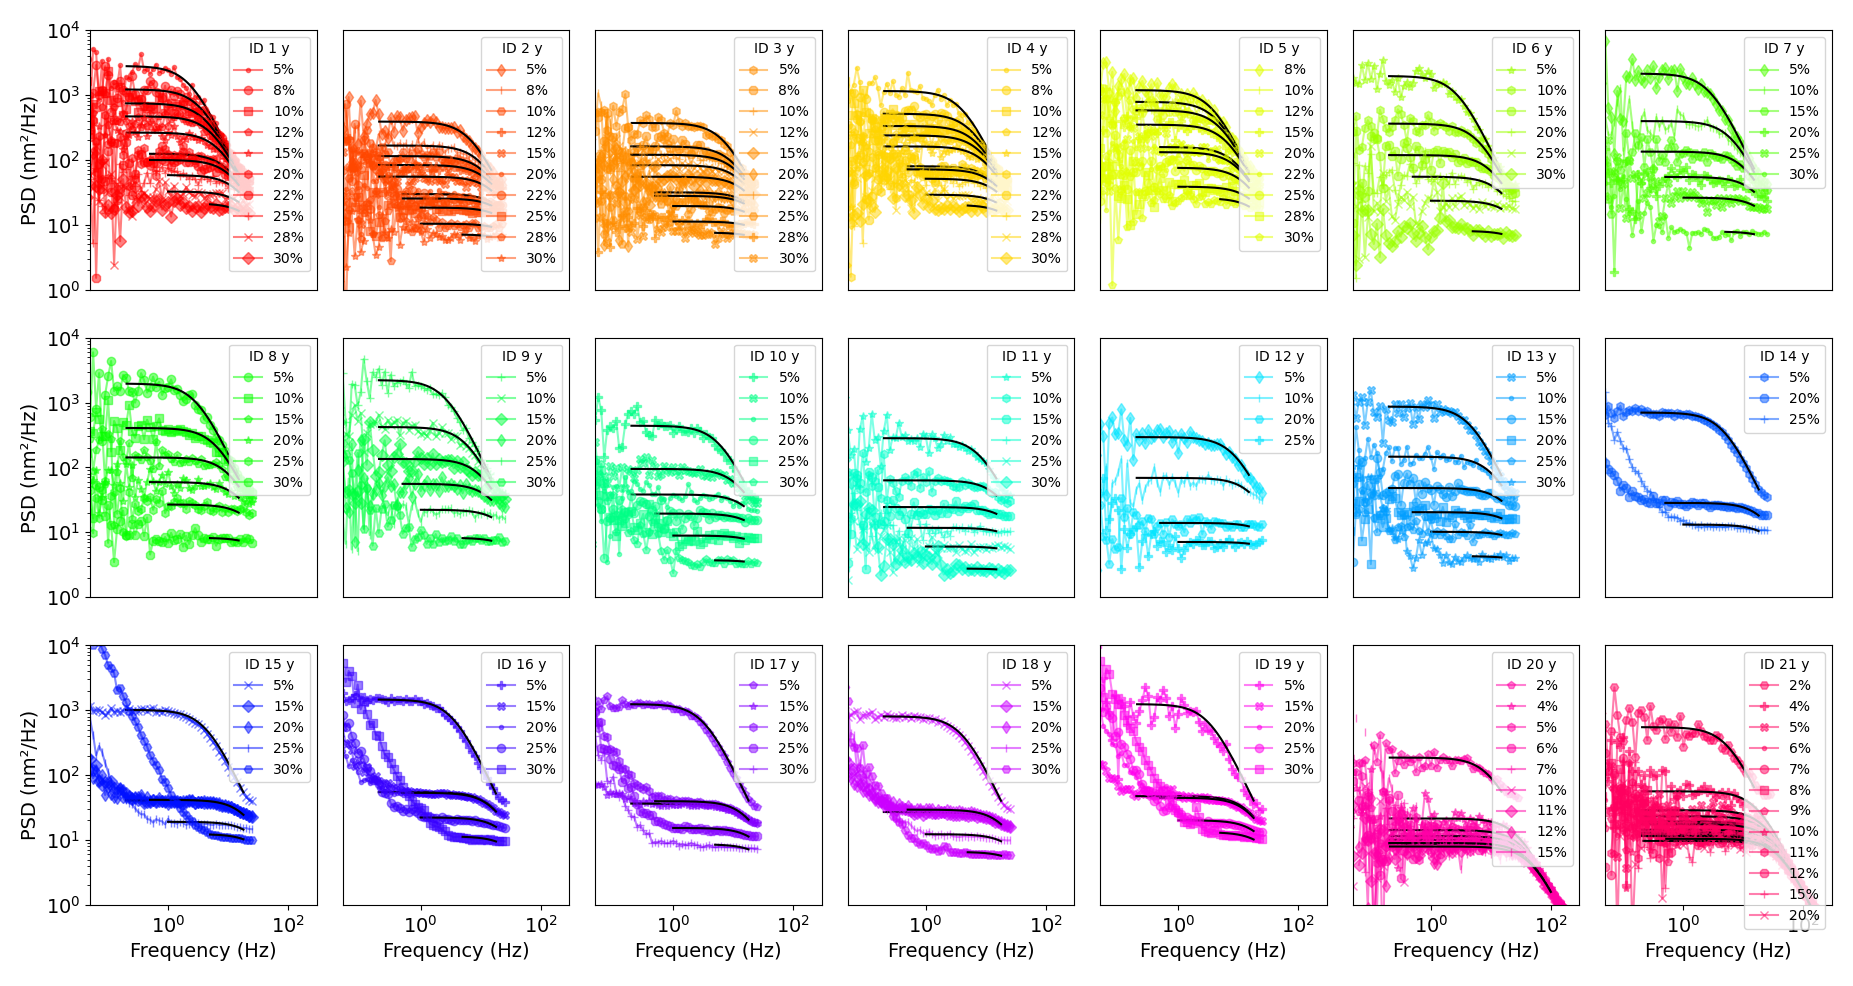
\includegraphics[width=1\linewidth]{Figures/multispectrumy_Rapa.png}}
	\caption{Power Spectra Density of y fluctuations for 21 beads tethered by J-DNA functionalized with the FKBP12-FRB complex and subject to different applied acoustic power. Fits with Eq. \ref{eq:PSD} are superimposed, taking for each bead as fitting parameters : the bead radius $R_b$ and the pendulum stiffness $k_i$ for each power.}
	\label{fig:FitSpectra_y}
\end{sidewaysfigure}

\begin{figure}[hbt!]
	\centering
	\centerline {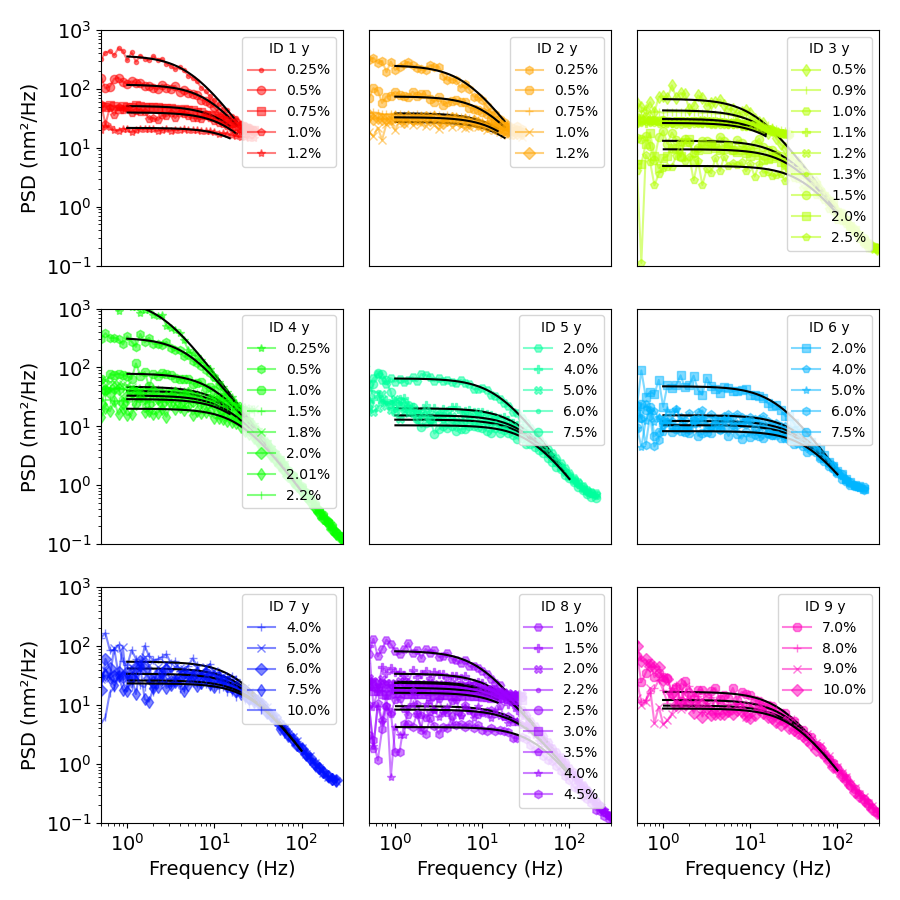
\includegraphics[width=1\linewidth]{Figures/multispectrumy_Nef.png}}
	\caption{%{\color{red}For information, possibly removed in final version} .
	Power Spectra Density of y fluctuations for 9 beads tethered by J-DNA functionalized with the Nef-Nef19 complex and subjected to different applied acoustic powers. Fits with Eq. \ref{eq:PSD} are superimposed, taking for each bead as fitting parameters : the bead radius $R$ and the pendulum stiffness $k_i$ for each power.}
	\label{fig:FitSpectraNef}	
\end{figure}

\begin{sidewaysfigure}[hbt!]
	\centering
	\centerline {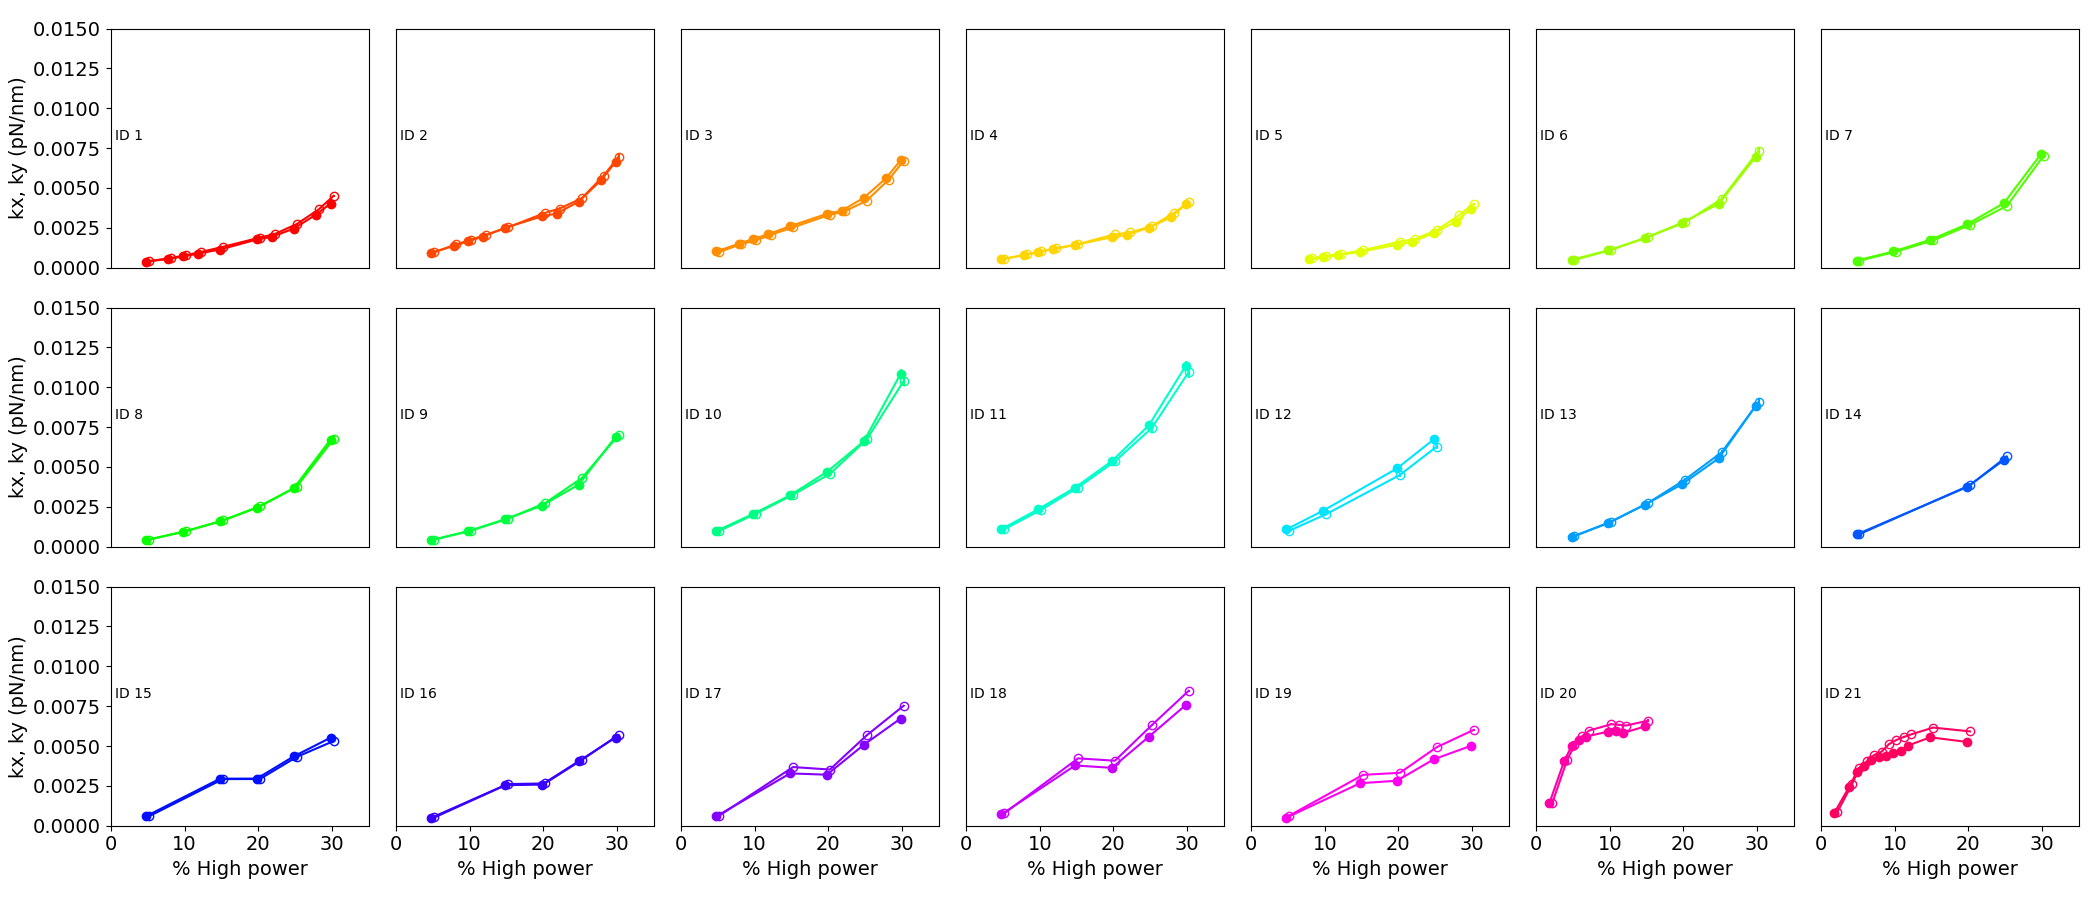
\includegraphics[width=1\linewidth]{Figures/Power_Stiffness_Ter_Rapa.png}}
	\caption{Stiffness of the pendulum from PSD fit as a function of applied acoustic power for 21 beads tethered by J-DNA functionalized with the FKBP12-Rapamycin-FRB complex. Plain symbols: stiffness obtained from PSD of x fluctuations. Empty symbols: stiffness obtained from PSD of y fluctuations.}
	\label{fig:PowerStiffness}	
\end{sidewaysfigure}

\begin{sidewaysfigure}[hbt!]
	\centering
	\centerline {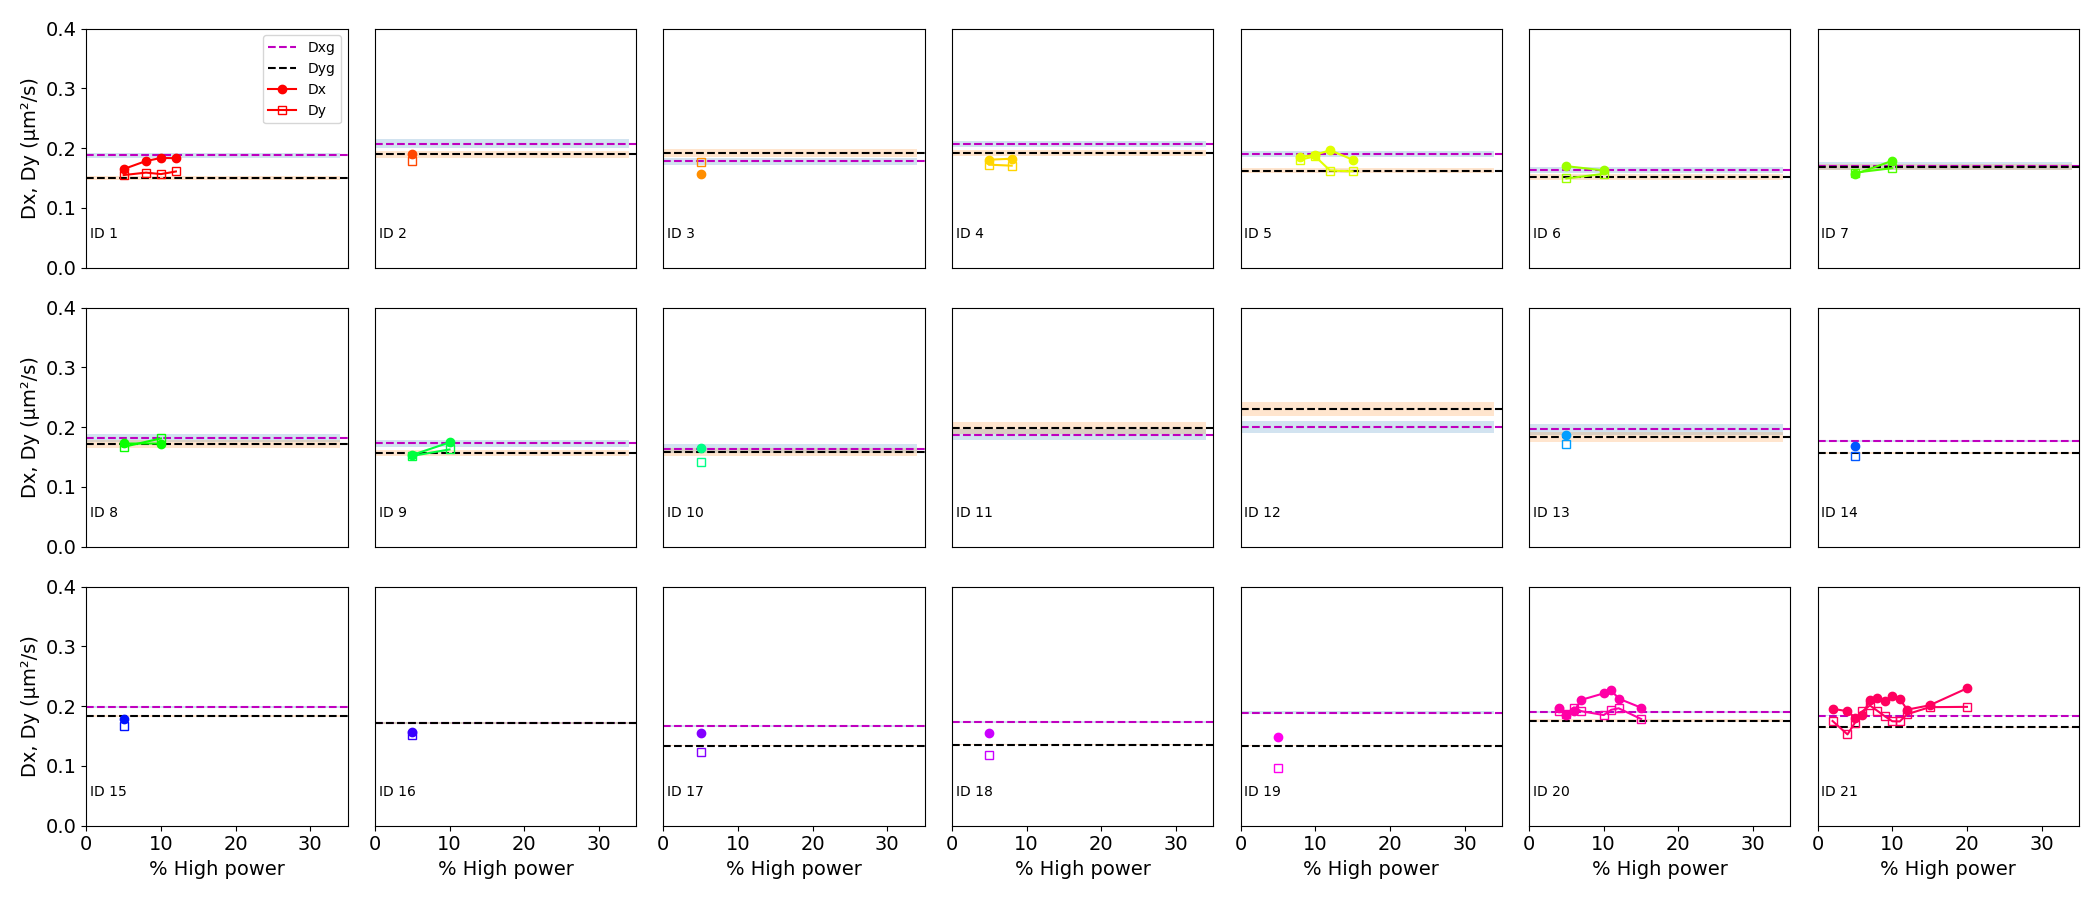
\includegraphics[width=1\linewidth]{Figures/Power_Friction_Bis_Rapa.png}}
	\caption{%{\color{red}For information, possibly removed in final version}
	Diffusion coefficient from PSD fit as a function of applied acoustic power for 21 beads tethered by J-DNA functionalized with the FKBP12-Rapamycin-FRB complex. Horizontal lines: diffusion coefficient calculated from the unique value of $R_x$, $R_y$ for each bead, as determined by the global fit of PSD. The shaded stripe indicates the error bar, based on the rrror on the fitting value of $R$ and the dependence of $D$ on J-DNA length, which depends on the power. Circles: individual PSD fit with one $D$ and one $k$, when the condition $f_c < f_{max}/2$ is fullfilled.}
	\label{fig:PowerDiffusion}
\end{sidewaysfigure}


\begin{figure}[hbt!]
	\centering
	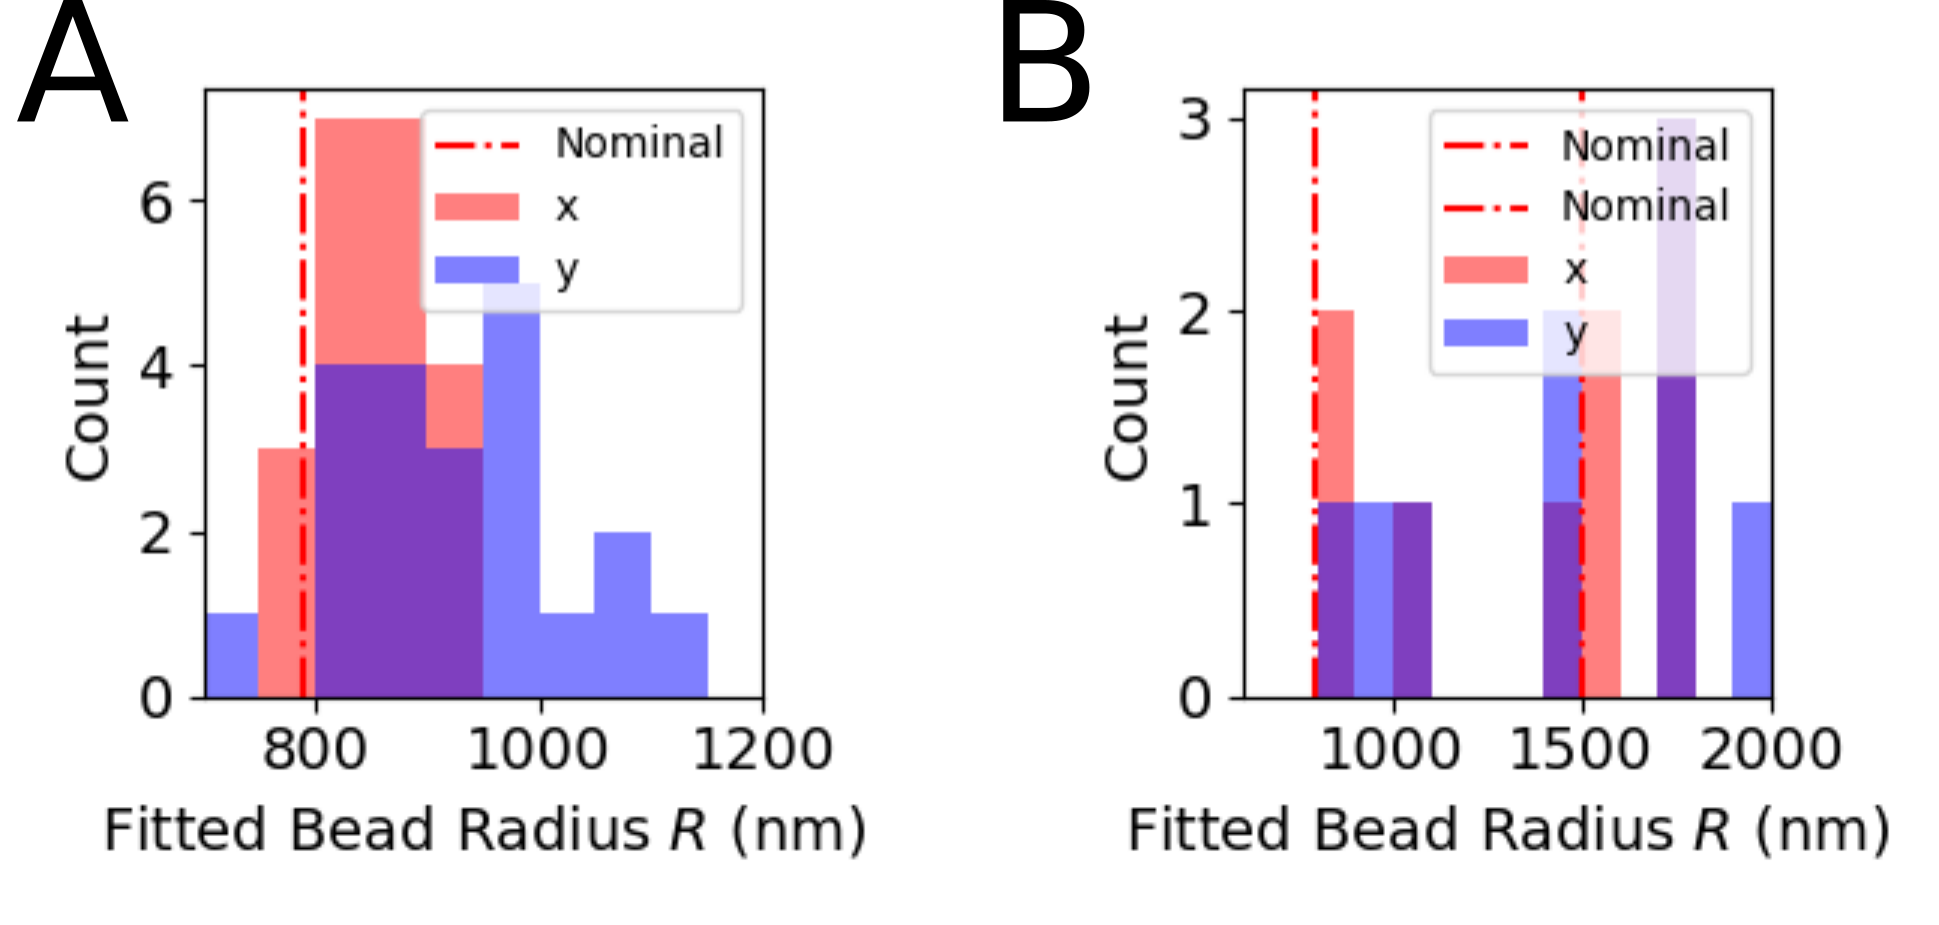
\includegraphics[width=0.6\linewidth]{Figures/fig_Radius.png}
	\caption{Distribution of apparent bead radius (in nm) retrieved from PSD fit. The nominal bead radius is indicated by the red dashed line. (A) 21 beads tethered by J-DNA functionalized with the FKBP12-Rapamycin-FRB complex. (B) 9 beads tethered by J-DNA functionalized with the Nef-Nef19. Two bead size were used in these measurements, represented by 2 red dashed lines.}
	\label{fig:Rdiffusion}
\end{figure}

%\begin{figure}[hbt!]
%	\centering
%	fig_Radius.png
%	\begin{subfigure}{0.45\textwidth}
%		\centering
%    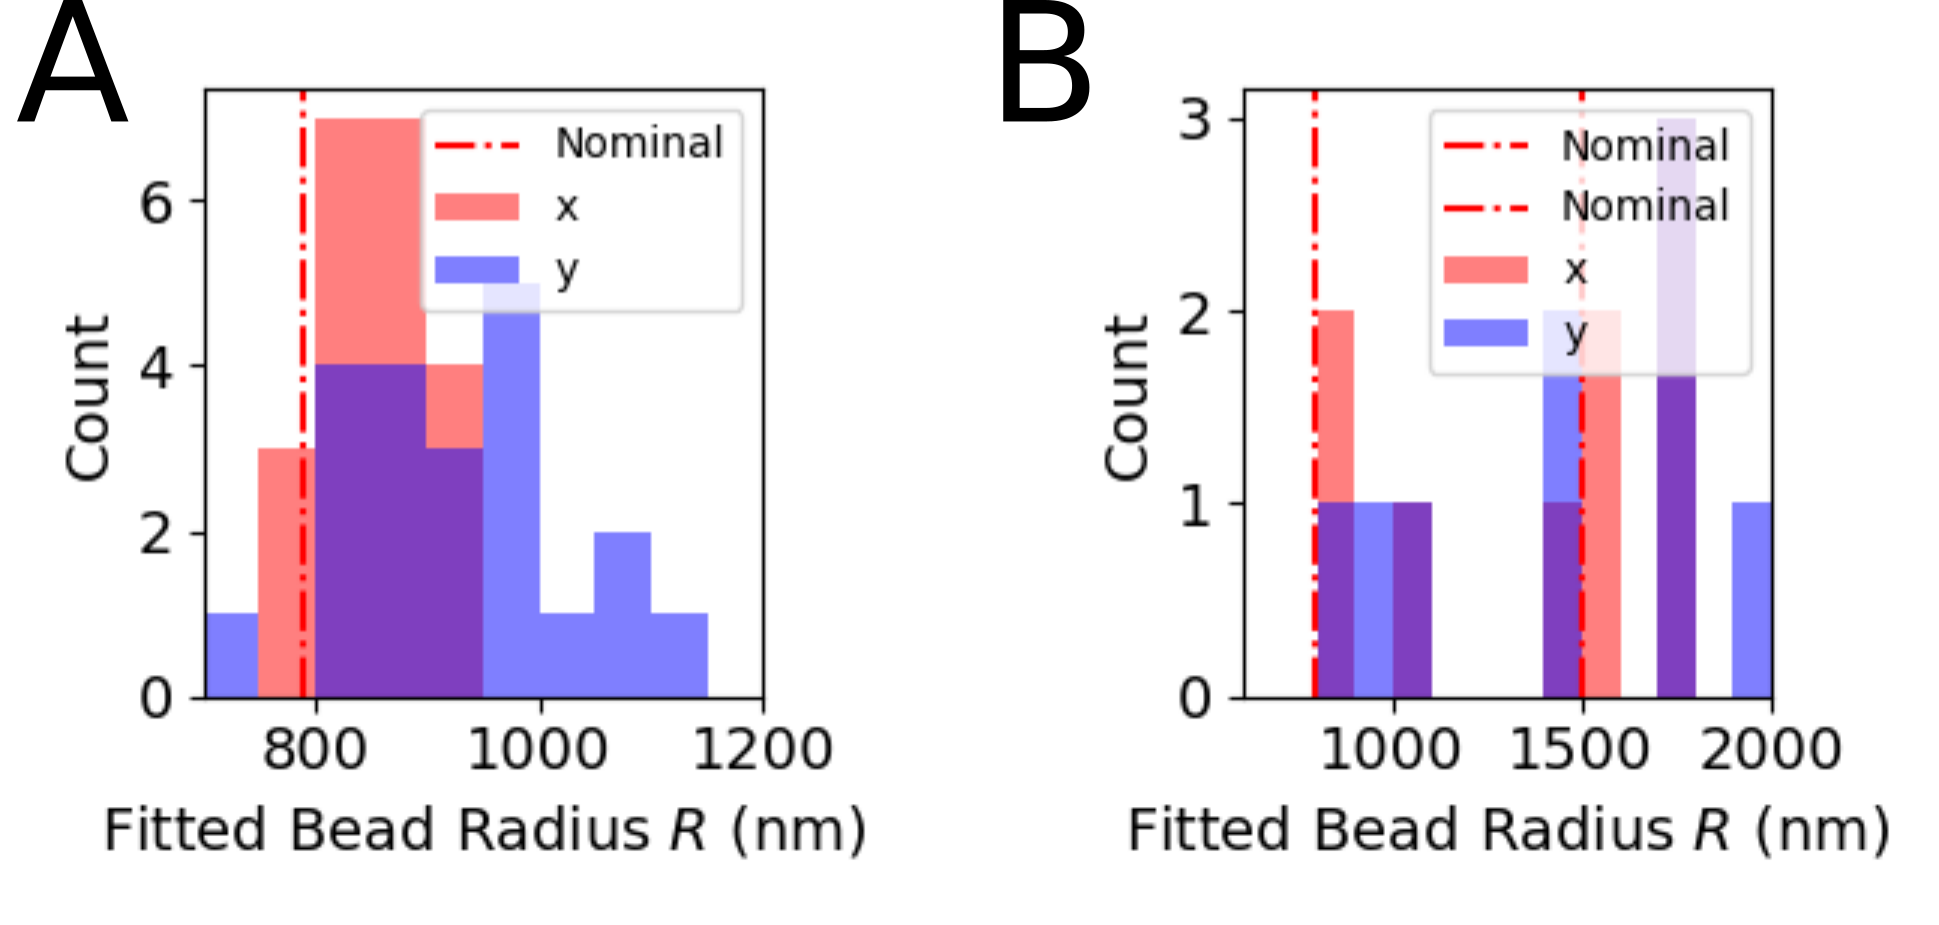
\includegraphics[width=0.6\linewidth]{Figures/fig_Radius.png}
%\caption{Nominal bead radius: 790 nm}
%%\label{fig:Rdiffusion}
%	\end{subfigure}
%	\begin{subfigure}{0.45\textwidth}
%		\centering
%	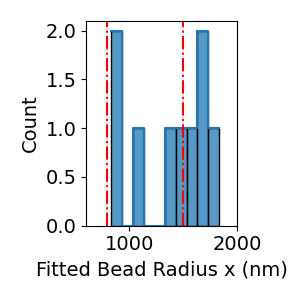
\includegraphics[width=0.6\linewidth]{Figures/RDiffusionHistx_Nef.png}
%\caption{Nominal bead radius: 790 and 1500 nm}
%%\label{fig:Rdiffusion}
%	\end{subfigure}
%	\caption{Distribution of apparent bead radius (in nm) retrieved from PSD fit. The nominal bead radius is indicated by the red dashed line. (A) 21 beads tethered by J-DNA functionalized with the FKBP12-Rapamycin-FRB complex. (B) 9 beads tethered by J-DNA functionalized with the Nef-Nef19. Two bead size were used in these measurements, represented by 2 red dashed lines.}
%	\label{fig:Rdiffusion}
%%	
\includegraphics[width=0.6\linewidth]{Figures/RDiffusionprecx_Rapa.png}
%
%\end{figure}

\begin{figure}[hbt!]
	\centering
	%	
\includegraphics[width=0.6\linewidth]{Figures/RDiffusionprecx_Rapa.png}

\end{figure}

%\begin{figure}[hbt!]
%	\centering
%	\centerline {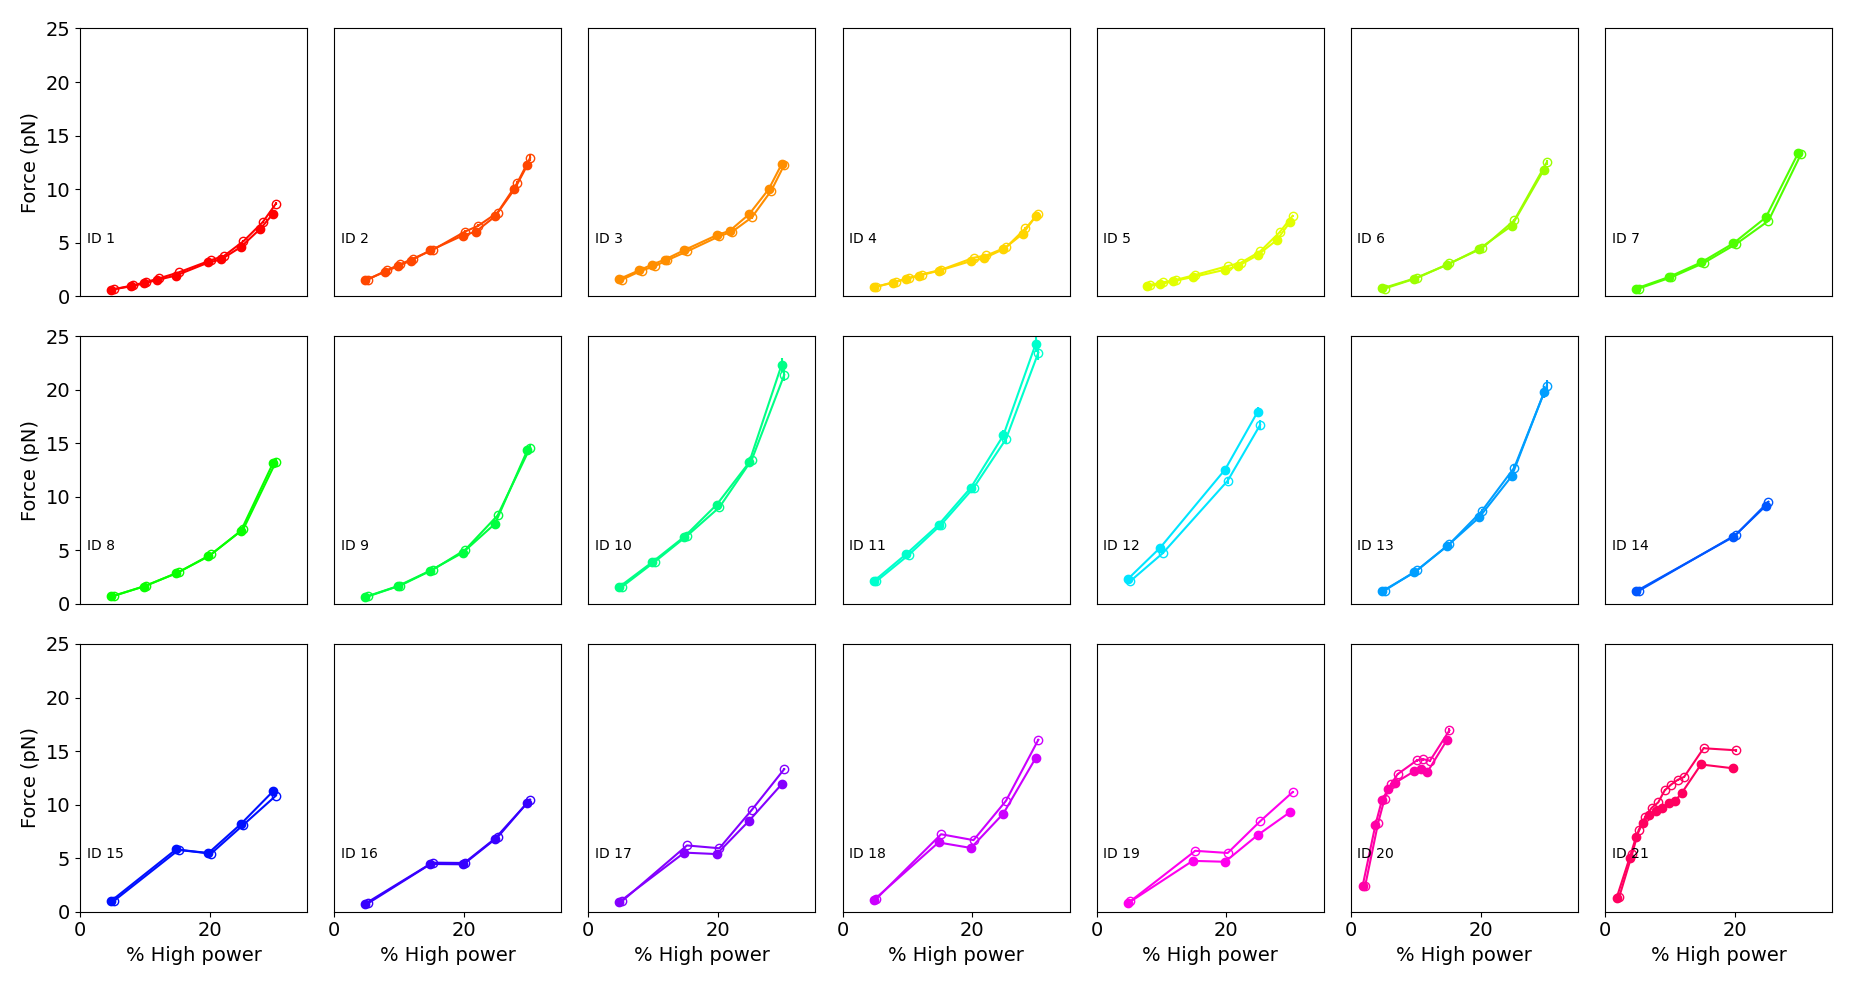
\includegraphics[width=1.2\linewidth]{Figures/Power_vs_Force_Bis_Rapa.png}}
%	\caption{Calibrated force (in pN) as a function of applied acoustic power for 21 beads tethered by J-DNA  functionalized with the FKBP12-Rapamycin-FRB complex.}
%	\label{fig:PowerForce}	
%\end{figure}

\begin{sidewaysfigure}[hbt!]
	\centering
	\centerline {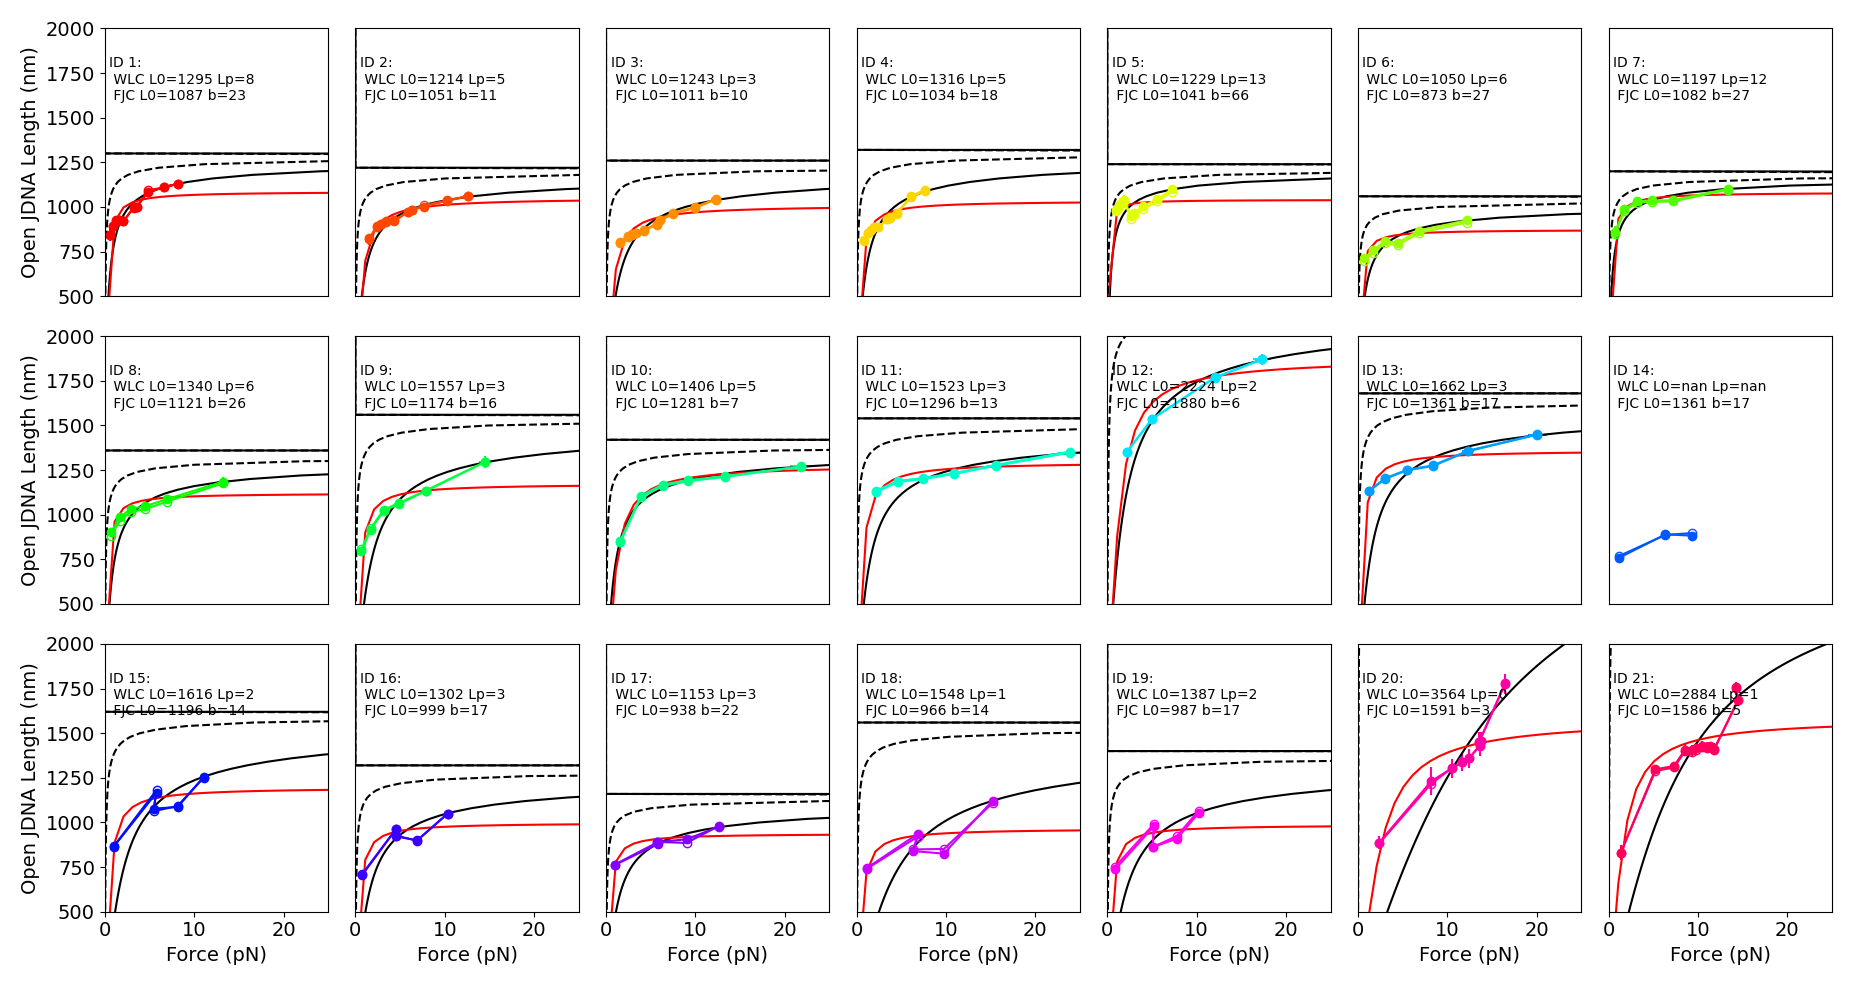
\includegraphics[width=1\linewidth]{Figures/Force_Lengths_Bis_Rapa.png}}
	\caption{Open J-DNA length (in nm) as a funtion of calibrated force for 21 beads tethered by J-DNA and subjected to different acoustic powers. Fit with a worm-like chain (WLC) model is superimposed to the data (black plain line), following the approximation: 
	$ F = \frac{k_B T}{L_p} \left[ \frac{1}{4(1-z/L_0)^2} - \frac{1}{4} + \frac{z}{L_0} \right] $ \cite{bouchiat1999}. The dashed curve represents the WLC model using $L_p=50$ nm and the previously obtained $L_0$.
	%\[ \frac{1}{4(1-z/L_0)^2} - \frac{1}{4} + \frac{z}{L_0}\] $. 
	The contour length $L_0$ and the persistence length $L_p$, extracted from the fit and expressed in nm, are indicated for each scaffold. ALternatively, a free joint chain (FJC) model is fitted, with Eq. $x = L(\coth \frac{Fb}{k_B T} - \frac{k_B T}{Fb})$, with $L$ the contour length and $b$ the Kuhn length \cite{smith1992} (red plain line).}
	\label{fig:ForceLength}	
\end{sidewaysfigure}

\begin{figure}[hbt!]
	\centering
%	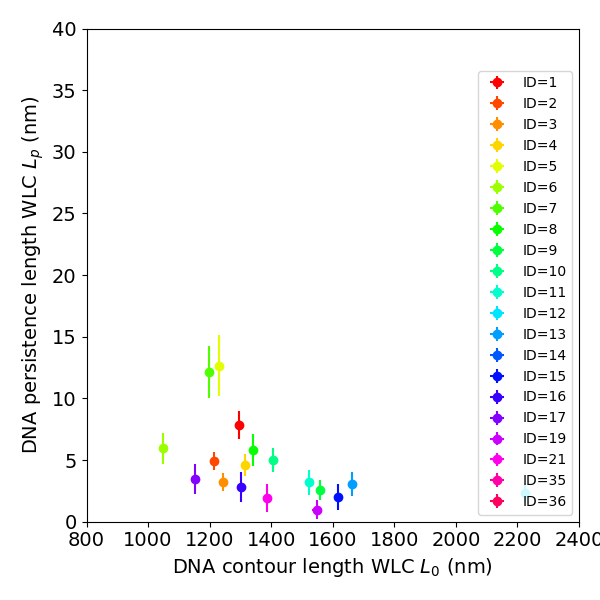
\includegraphics[width=0.6\linewidth]{Figures/Lp_vs_L0_Rapa.png}
	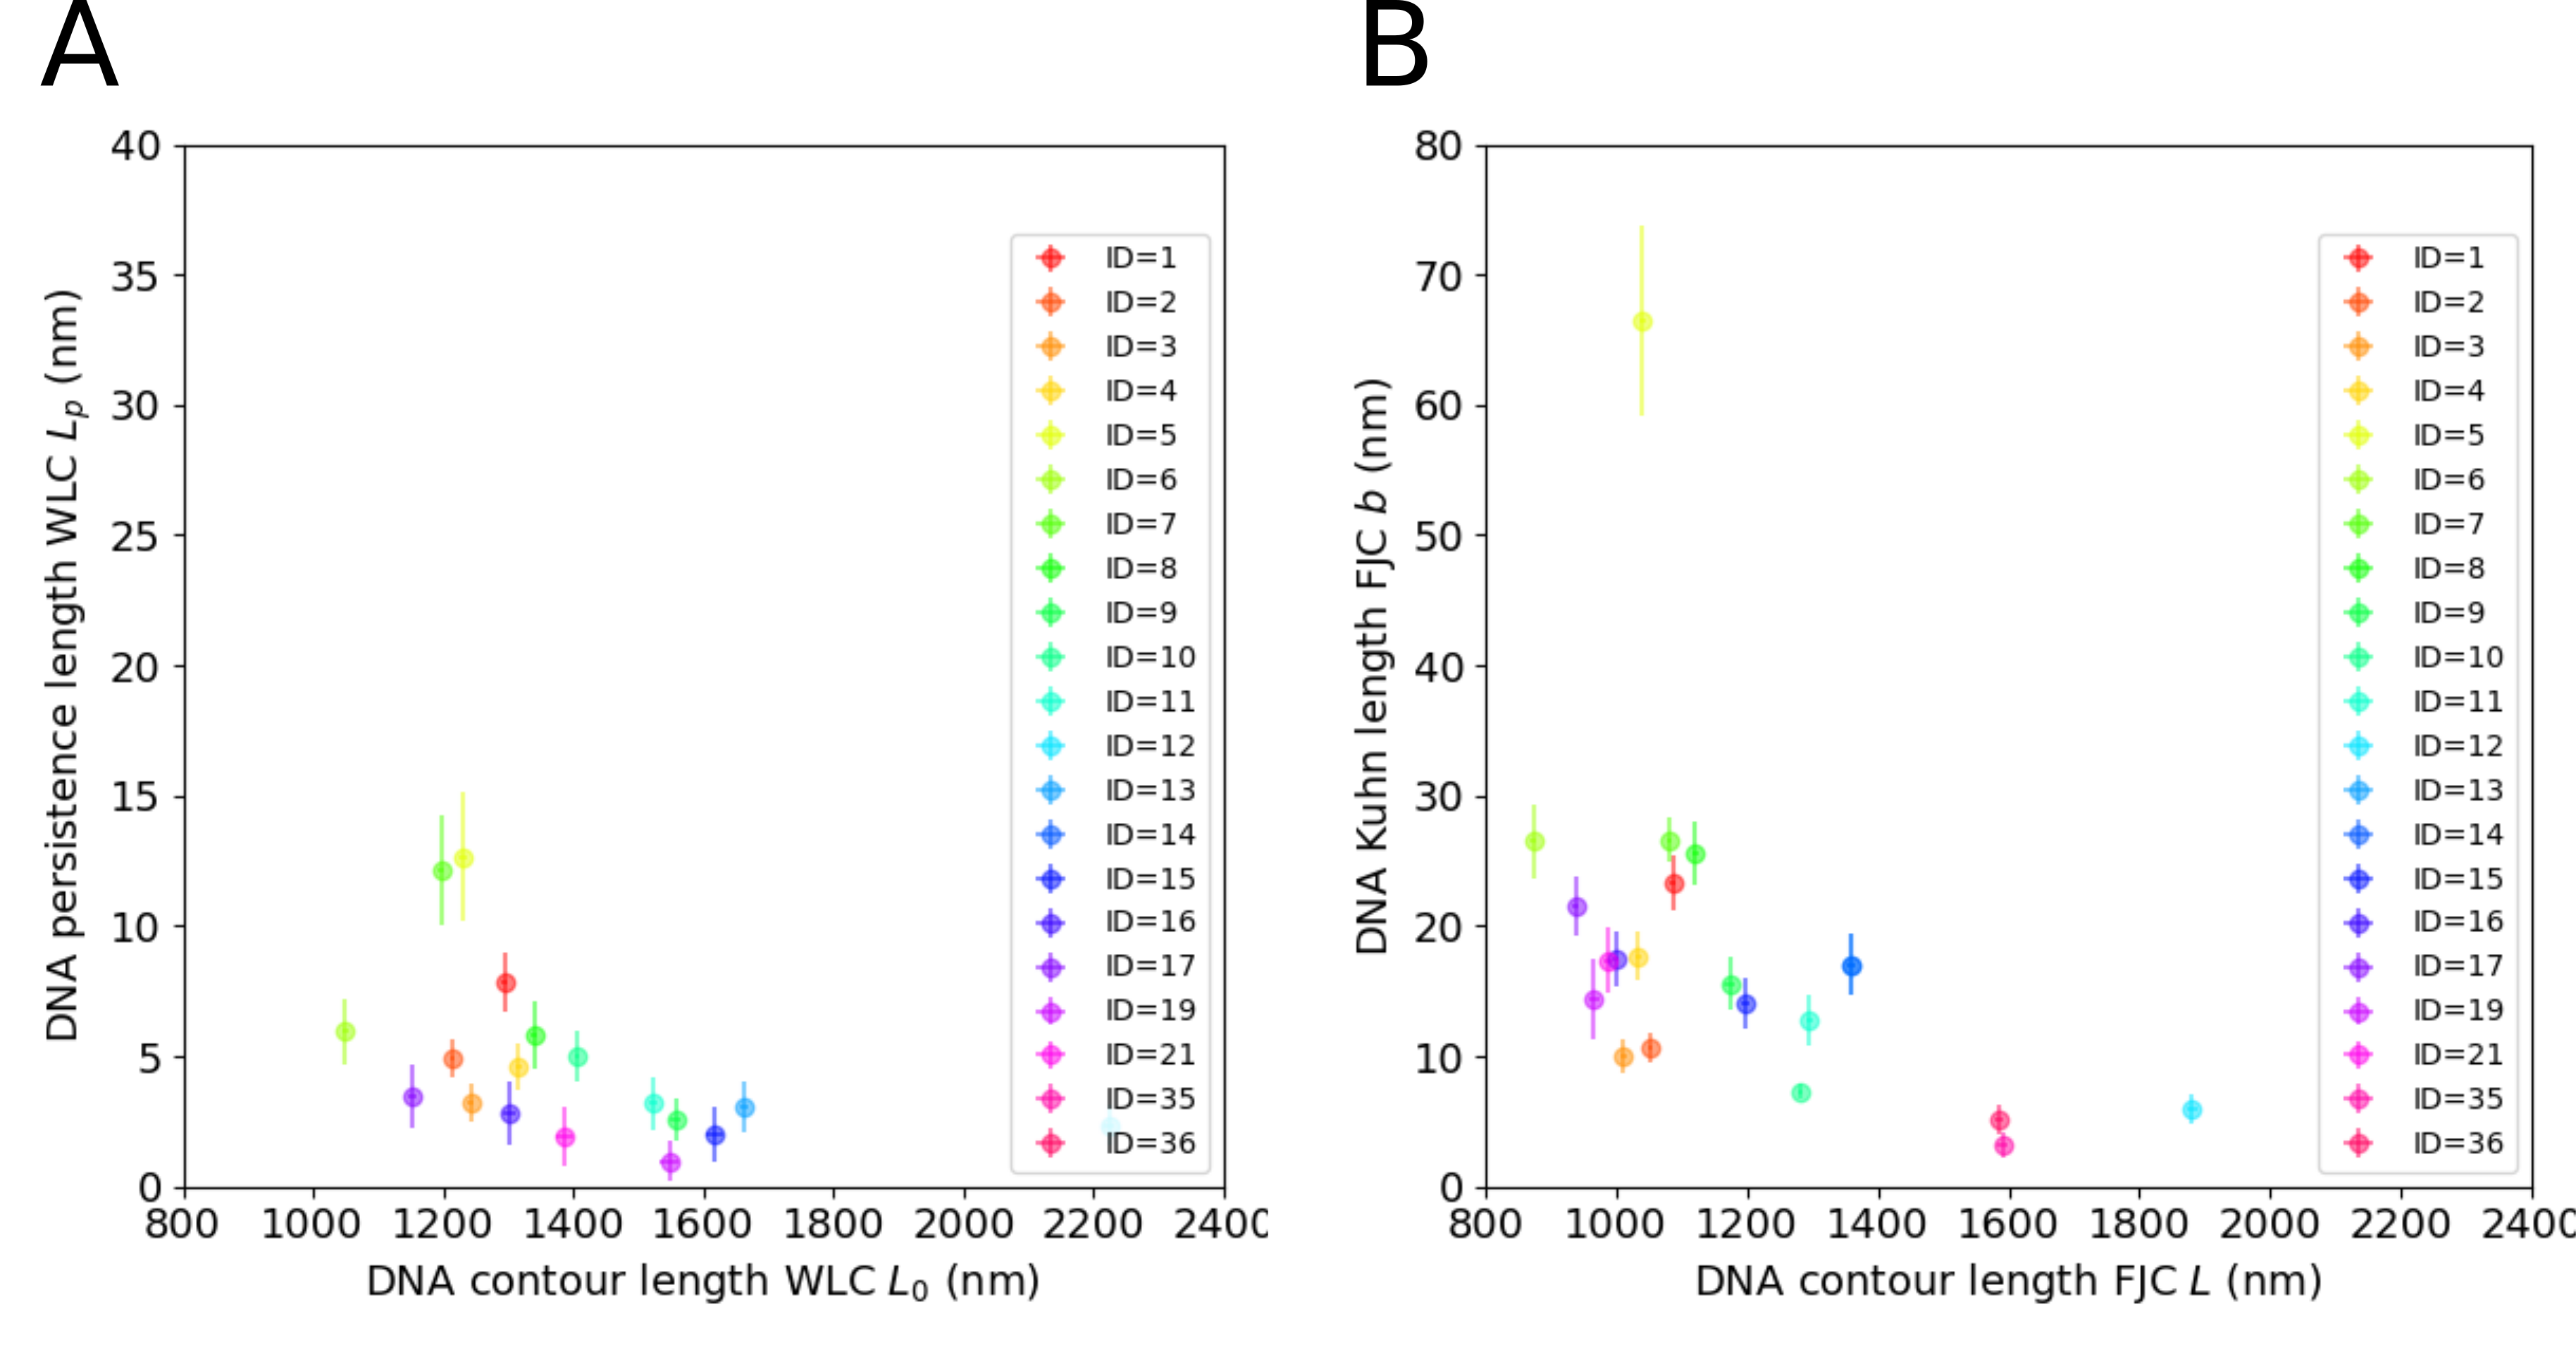
\includegraphics[width=1\linewidth]{Figures/fig_WLC_FJC.png}
	\caption{A. Relation between worm-like chain parameters contour length $L_0$ and persistence length $L_p$ characterizing individual J-DNA scaffolds functionalized with the FKBP12-Rapamycin-FRB complex. Relation between free-joints chain parameters $L$ and Kuhn length $L_p$ for the same scaffolds. }
	\label{fig:Lp_vs_L0}	
\end{figure}

\begin{sidewaysfigure}[hbt!]
	\centering
	\centerline {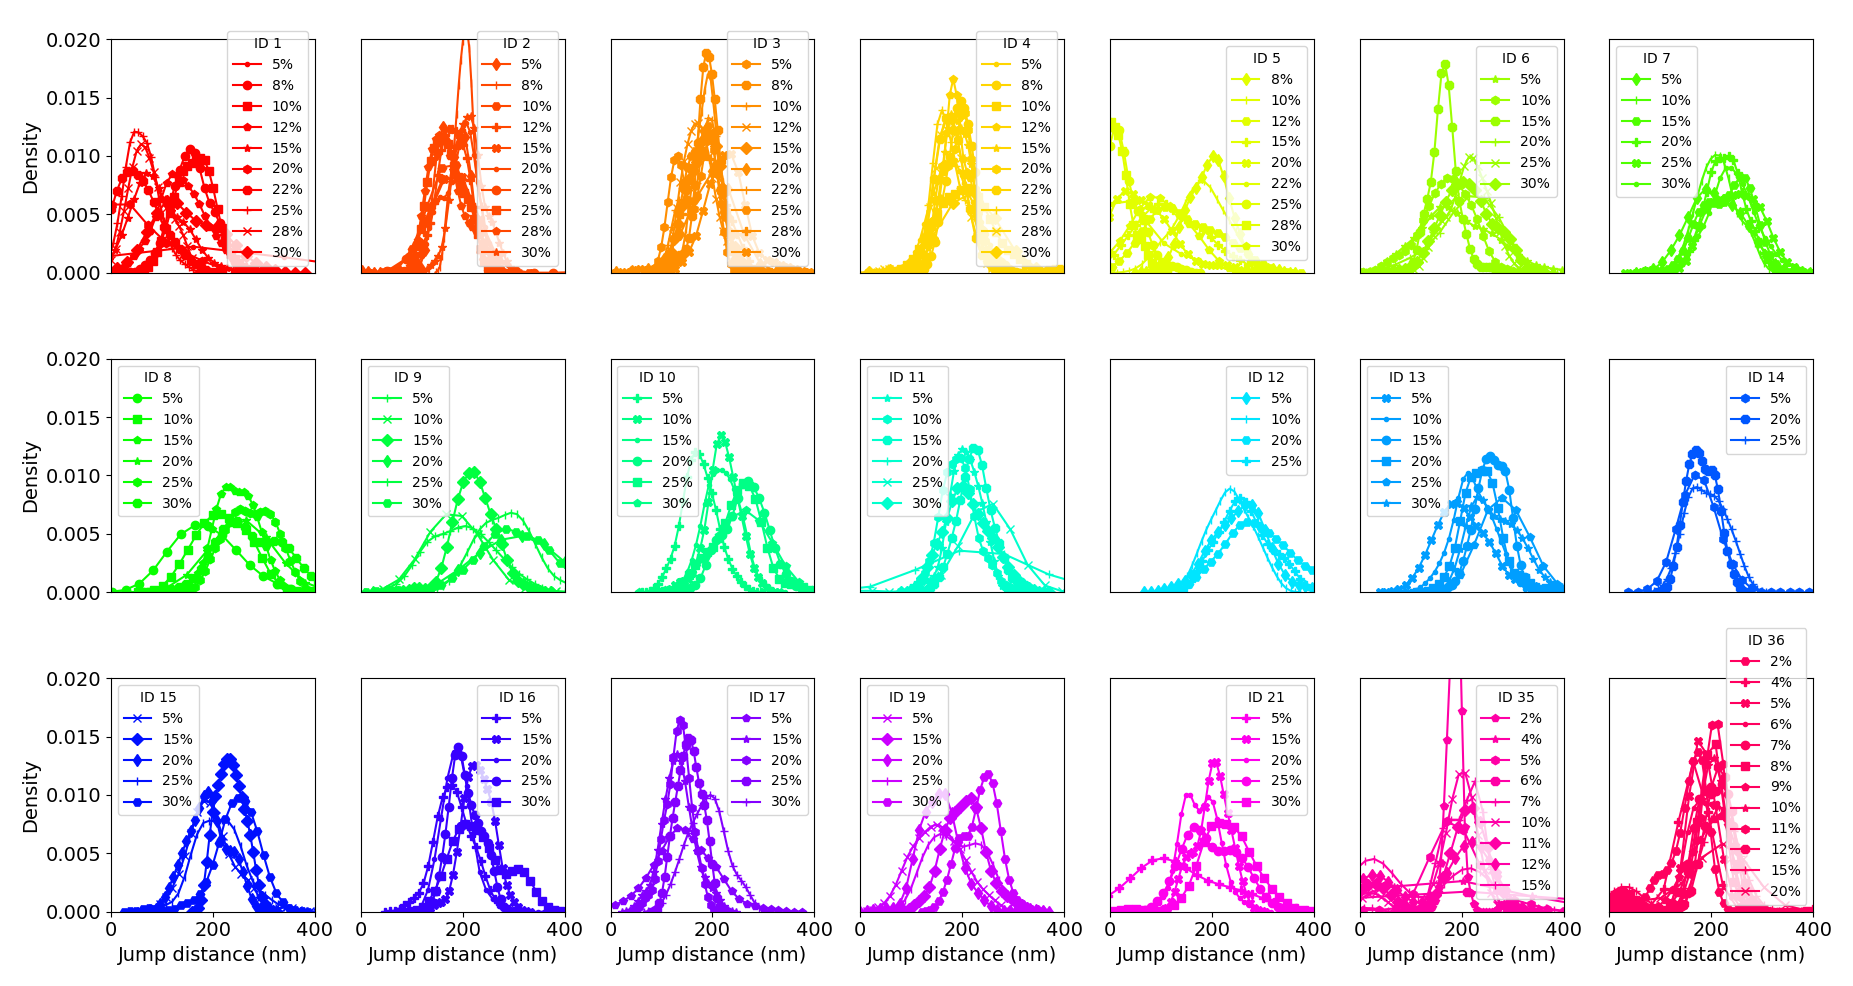
\includegraphics[width=1\linewidth]{Figures/multihistodzjump_Rapa.png}}
	\caption{Distribution density of jump distance of J-DNA opening (in nm) as a funtion of calibrated force for 21 beads tethered by J-DNA and subjected to different acoustic powers. Each symbol represents a different applied acoustic power.}
	\label{fig:JumpDistributions}	
\end{sidewaysfigure}

%\begin{figure}[hbt!]
%	\centering
%	\centerline {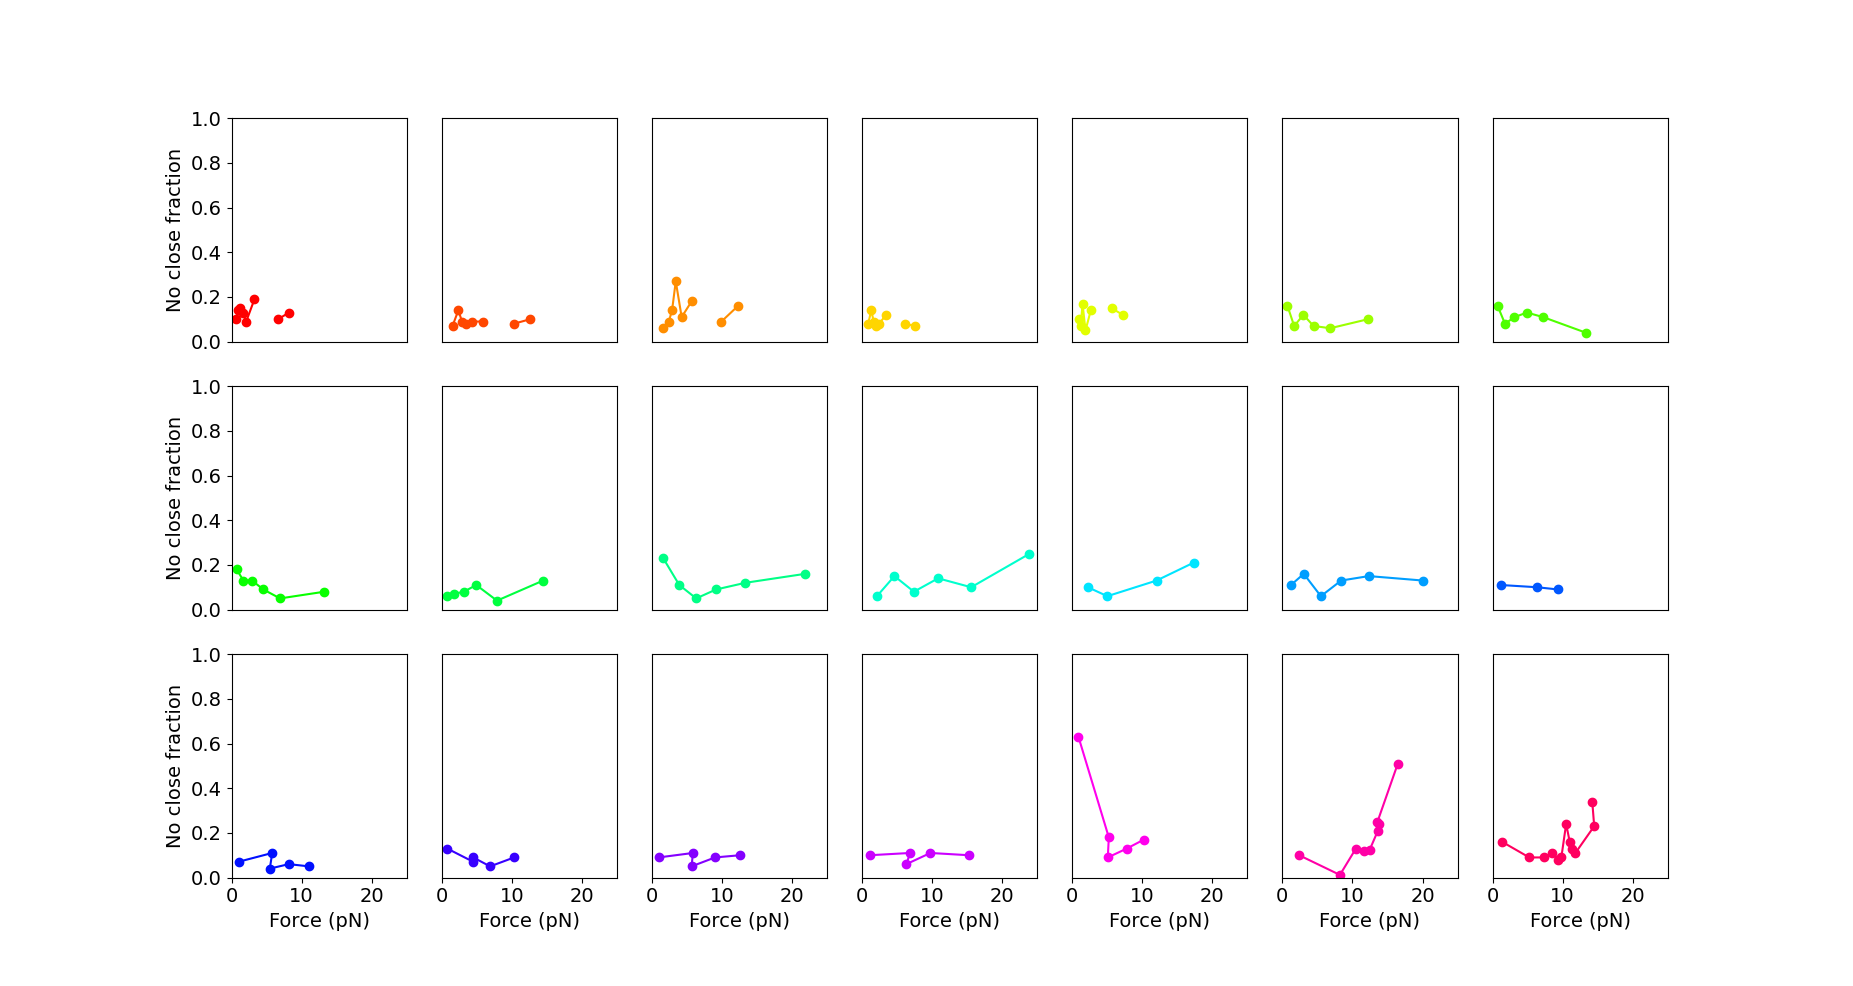
\includegraphics[width=1.2\linewidth]{Figures/No_Close_Fraction_Rapa.png}}
%	\caption{Fraction of non-closing events for 21 molecules and various applied acoustic power.}
%	\label{fig:MultiNoClose}	
%\end{figure}


\begin{sidewaysfigure}[hbt!]
	\centering
	\centerline {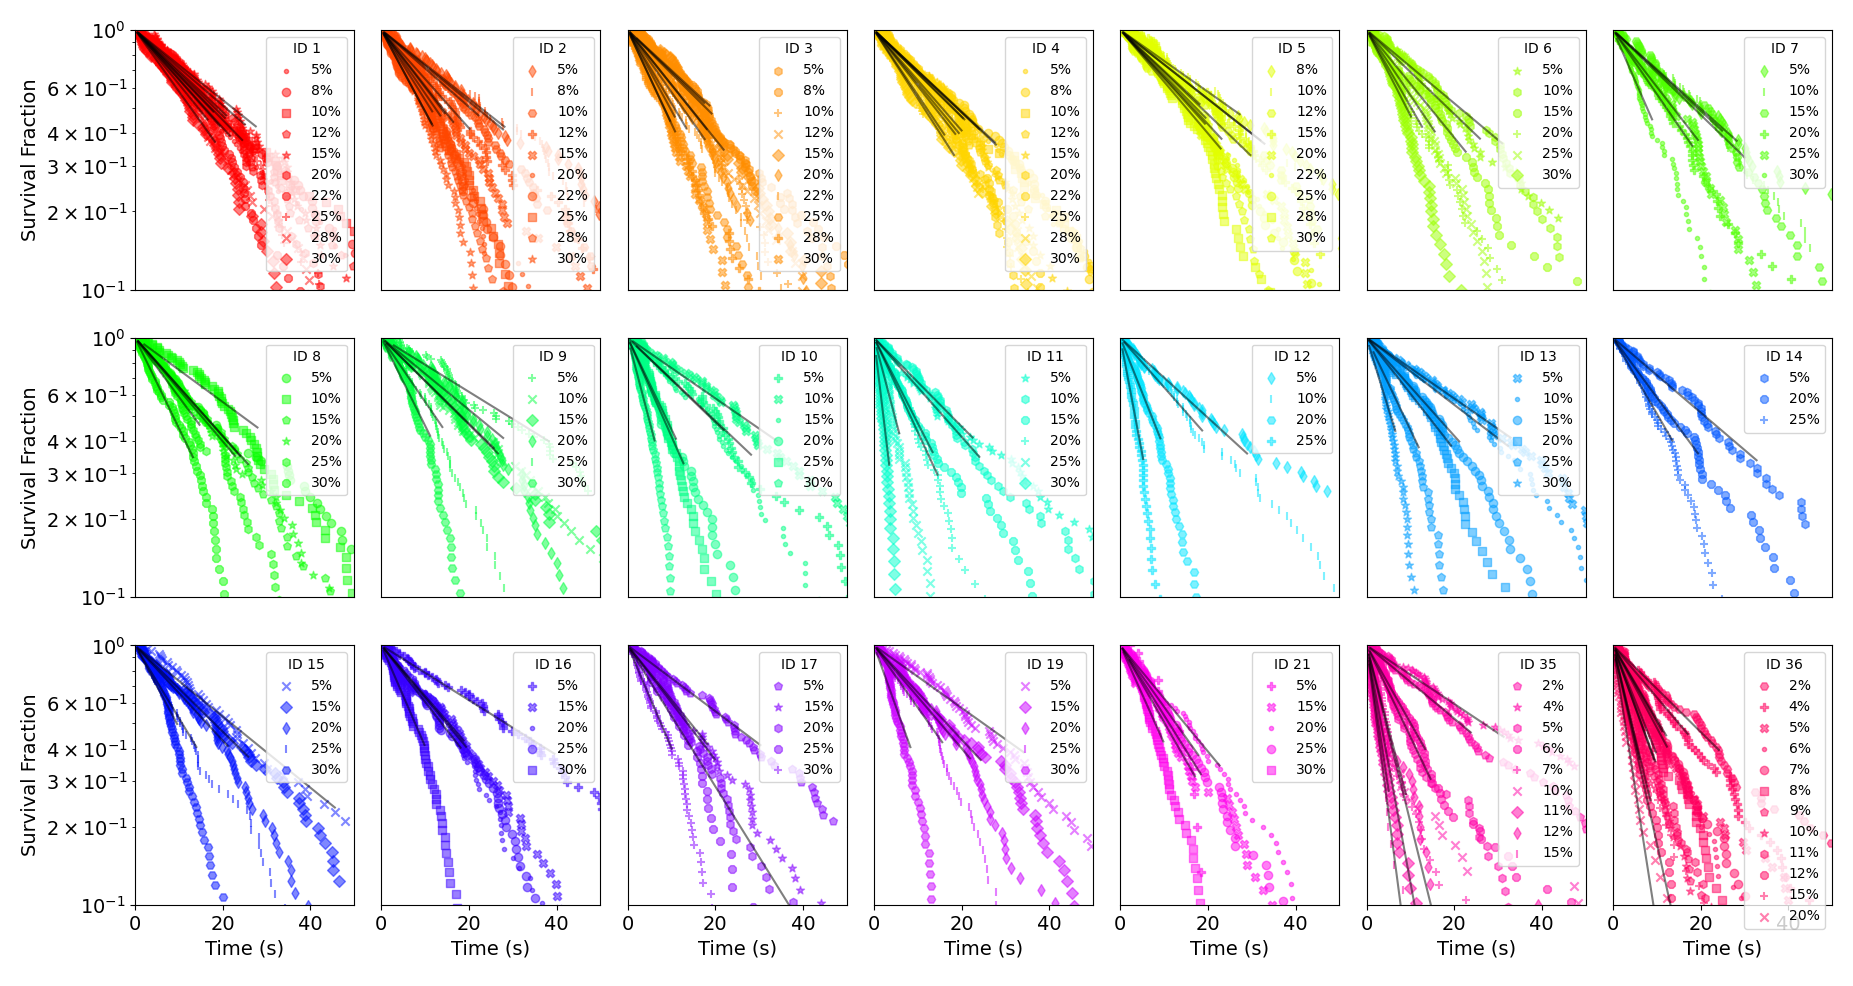
\includegraphics[width=1\linewidth]{Figures/multisurvival2Bis_Rapa.png}}
	\caption{Survival of FKBP12-Rapamycin-FRB bonds for 21 complexes and various applied acoustic power.}
	\label{fig:MultiSurvival}	
\end{sidewaysfigure}

\begin{sidewaysfigure}[hbt!]
	\centering
	\centerline {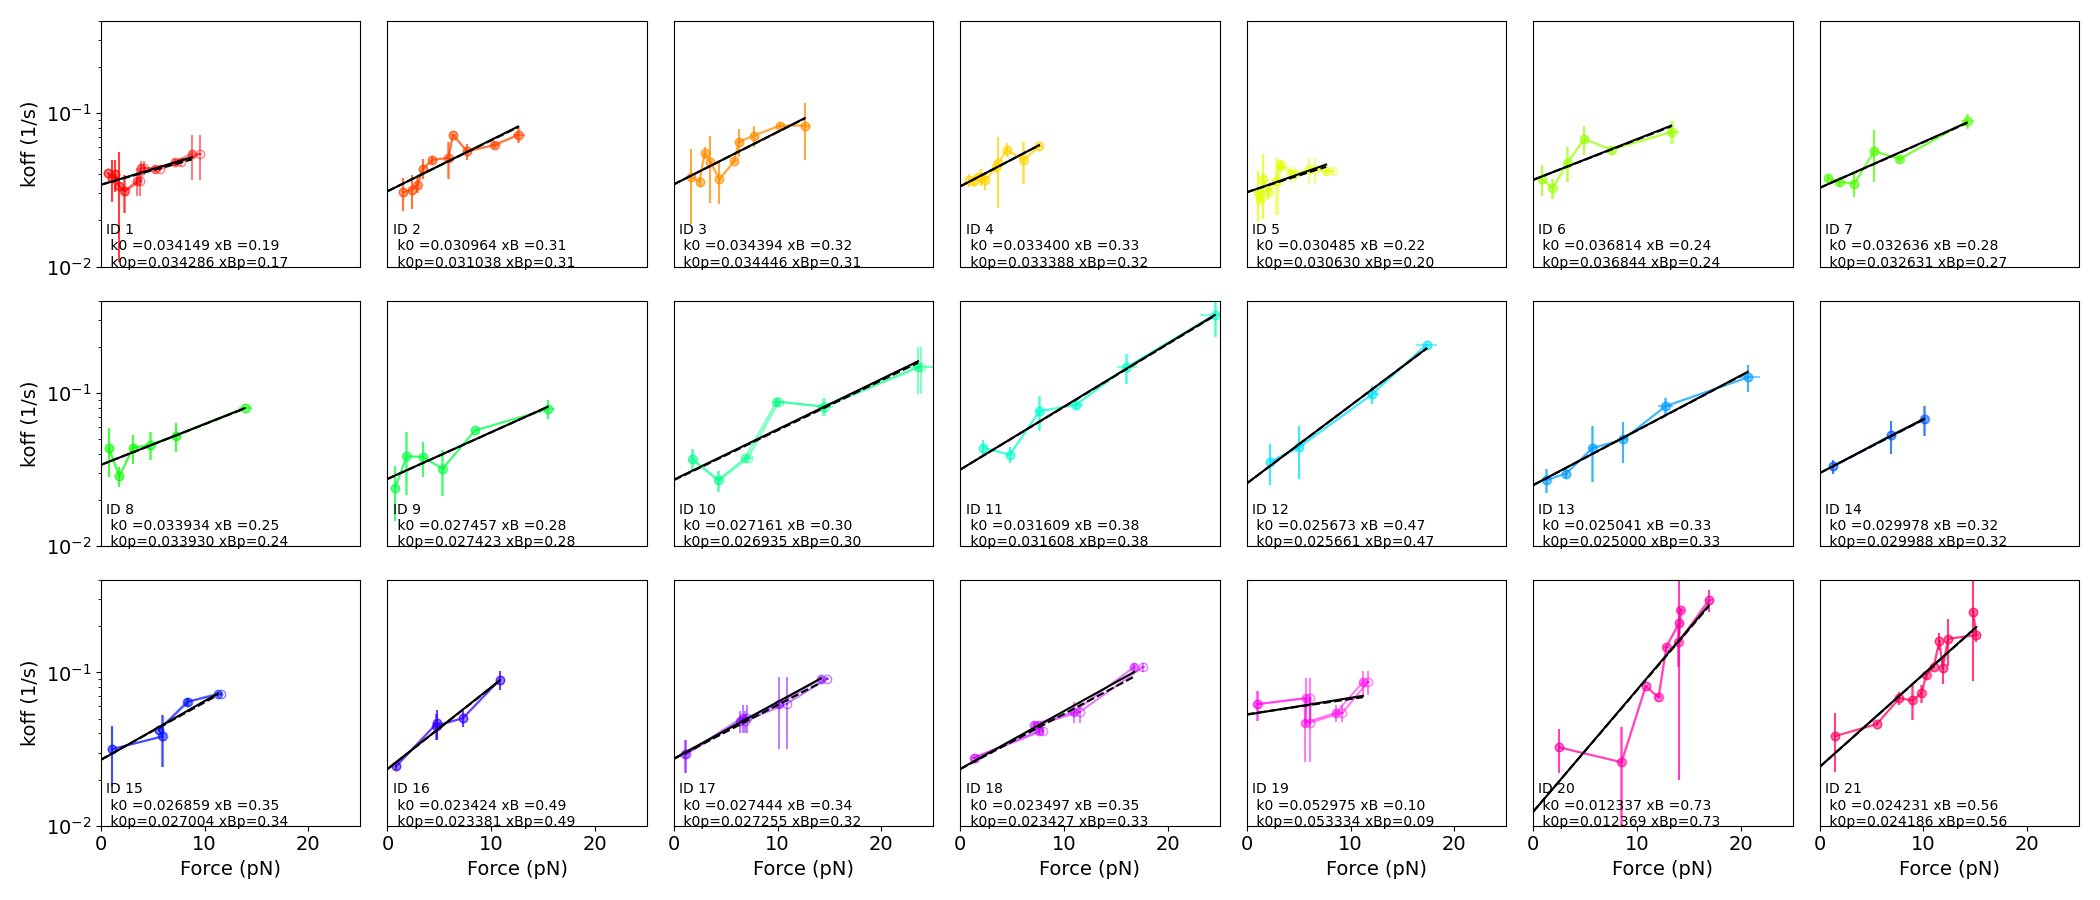
\includegraphics[width=1\linewidth]{Figures/offrate_vs_forceBis_Rapa.png}}
	\caption{Dependence of off-rate of FKBP12-Rapamycin-FRB bonds as a function of force for 21 complexes (plain symbols). Plain line indicates fit with the Bell equation. Empty symbols are calculated using the force projected along the main axis of the scaffold, considering the angle $\theta$. The dashed line represent the Bell fit for the projected force. Bell parameters $k^0_{\rm off}$ (in s$^{-1}$) and $x_b$ (in nm) are indicated in each case for non-projected or projected force. }
	\label{fig:offrate_force}	
\end{sidewaysfigure}

\begin{figure}[hbt!]
	\centering
	\centerline {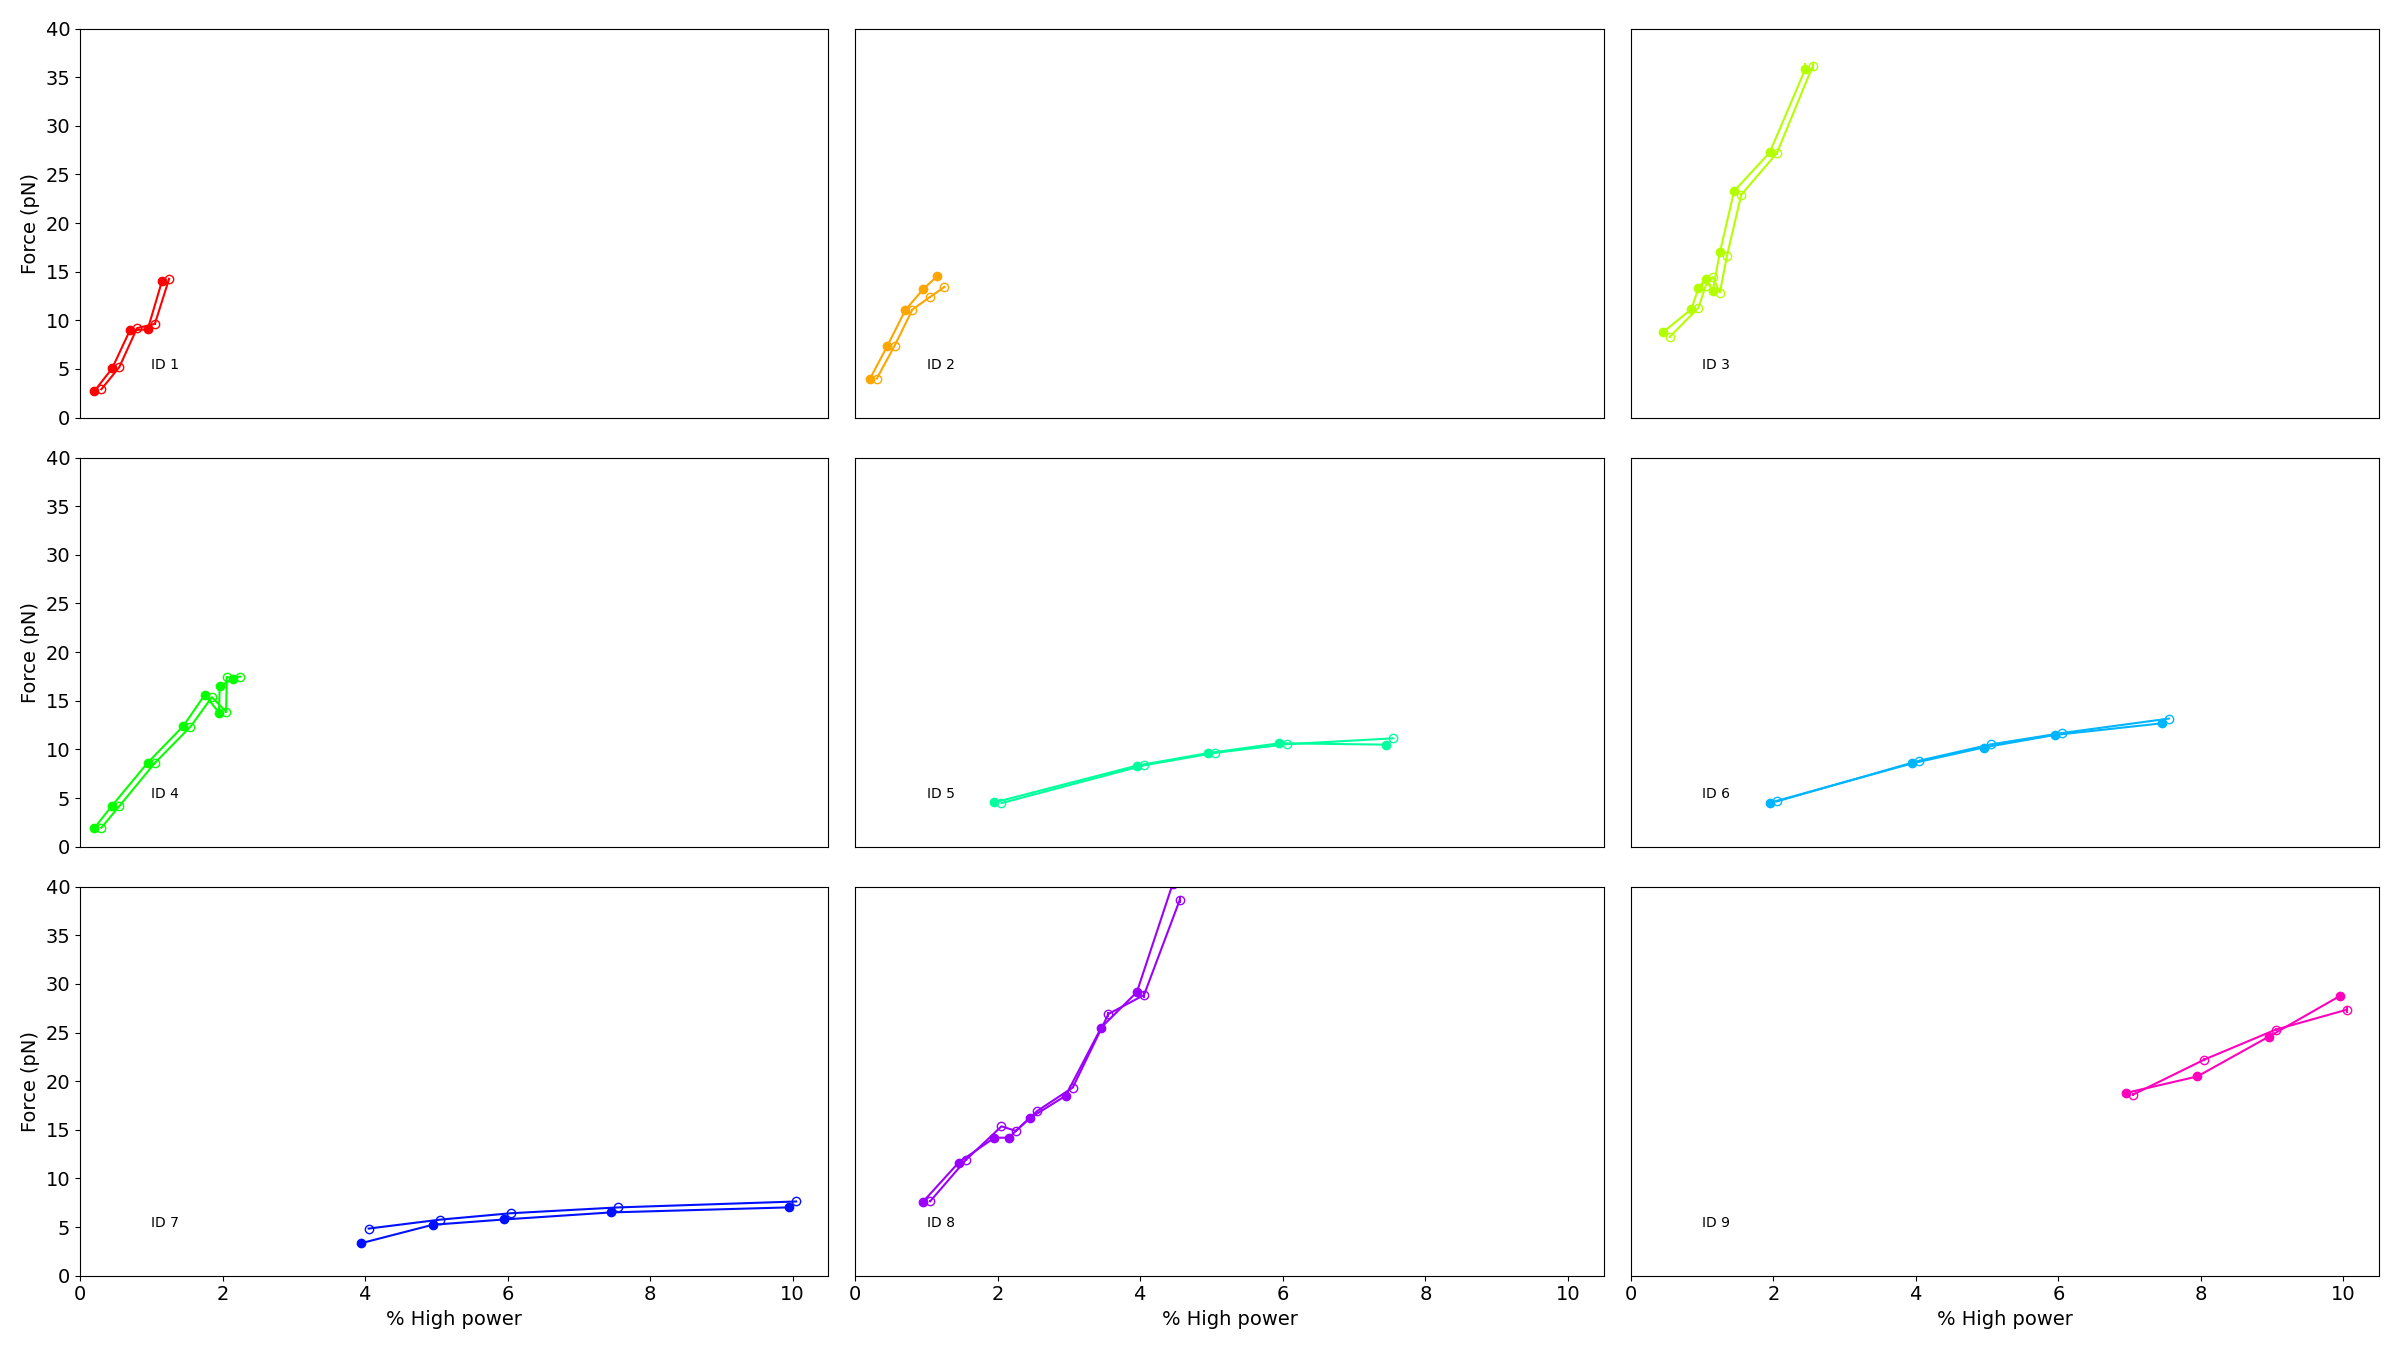
\includegraphics[width=1\linewidth]{Figures/Power_vs_Force_Bis_Nef.png}}
	\caption{Calibrated force (in pN) as a function of applied acoustic power for 9 beads tethered by J-DNA  functionalized with the Nef-Nef19 complex.  Plain symbols: force in x direction. Empty symbols: force in y direction. Notice that ID 5,6,7 correspond to $R= 900$ nm beads, while other IDs correspond to $R=1500$ nm.}
	\label{fig:PowerForce_Nef}	
\end{figure}

\begin{figure}[hbt!]
	\centering
	\centerline {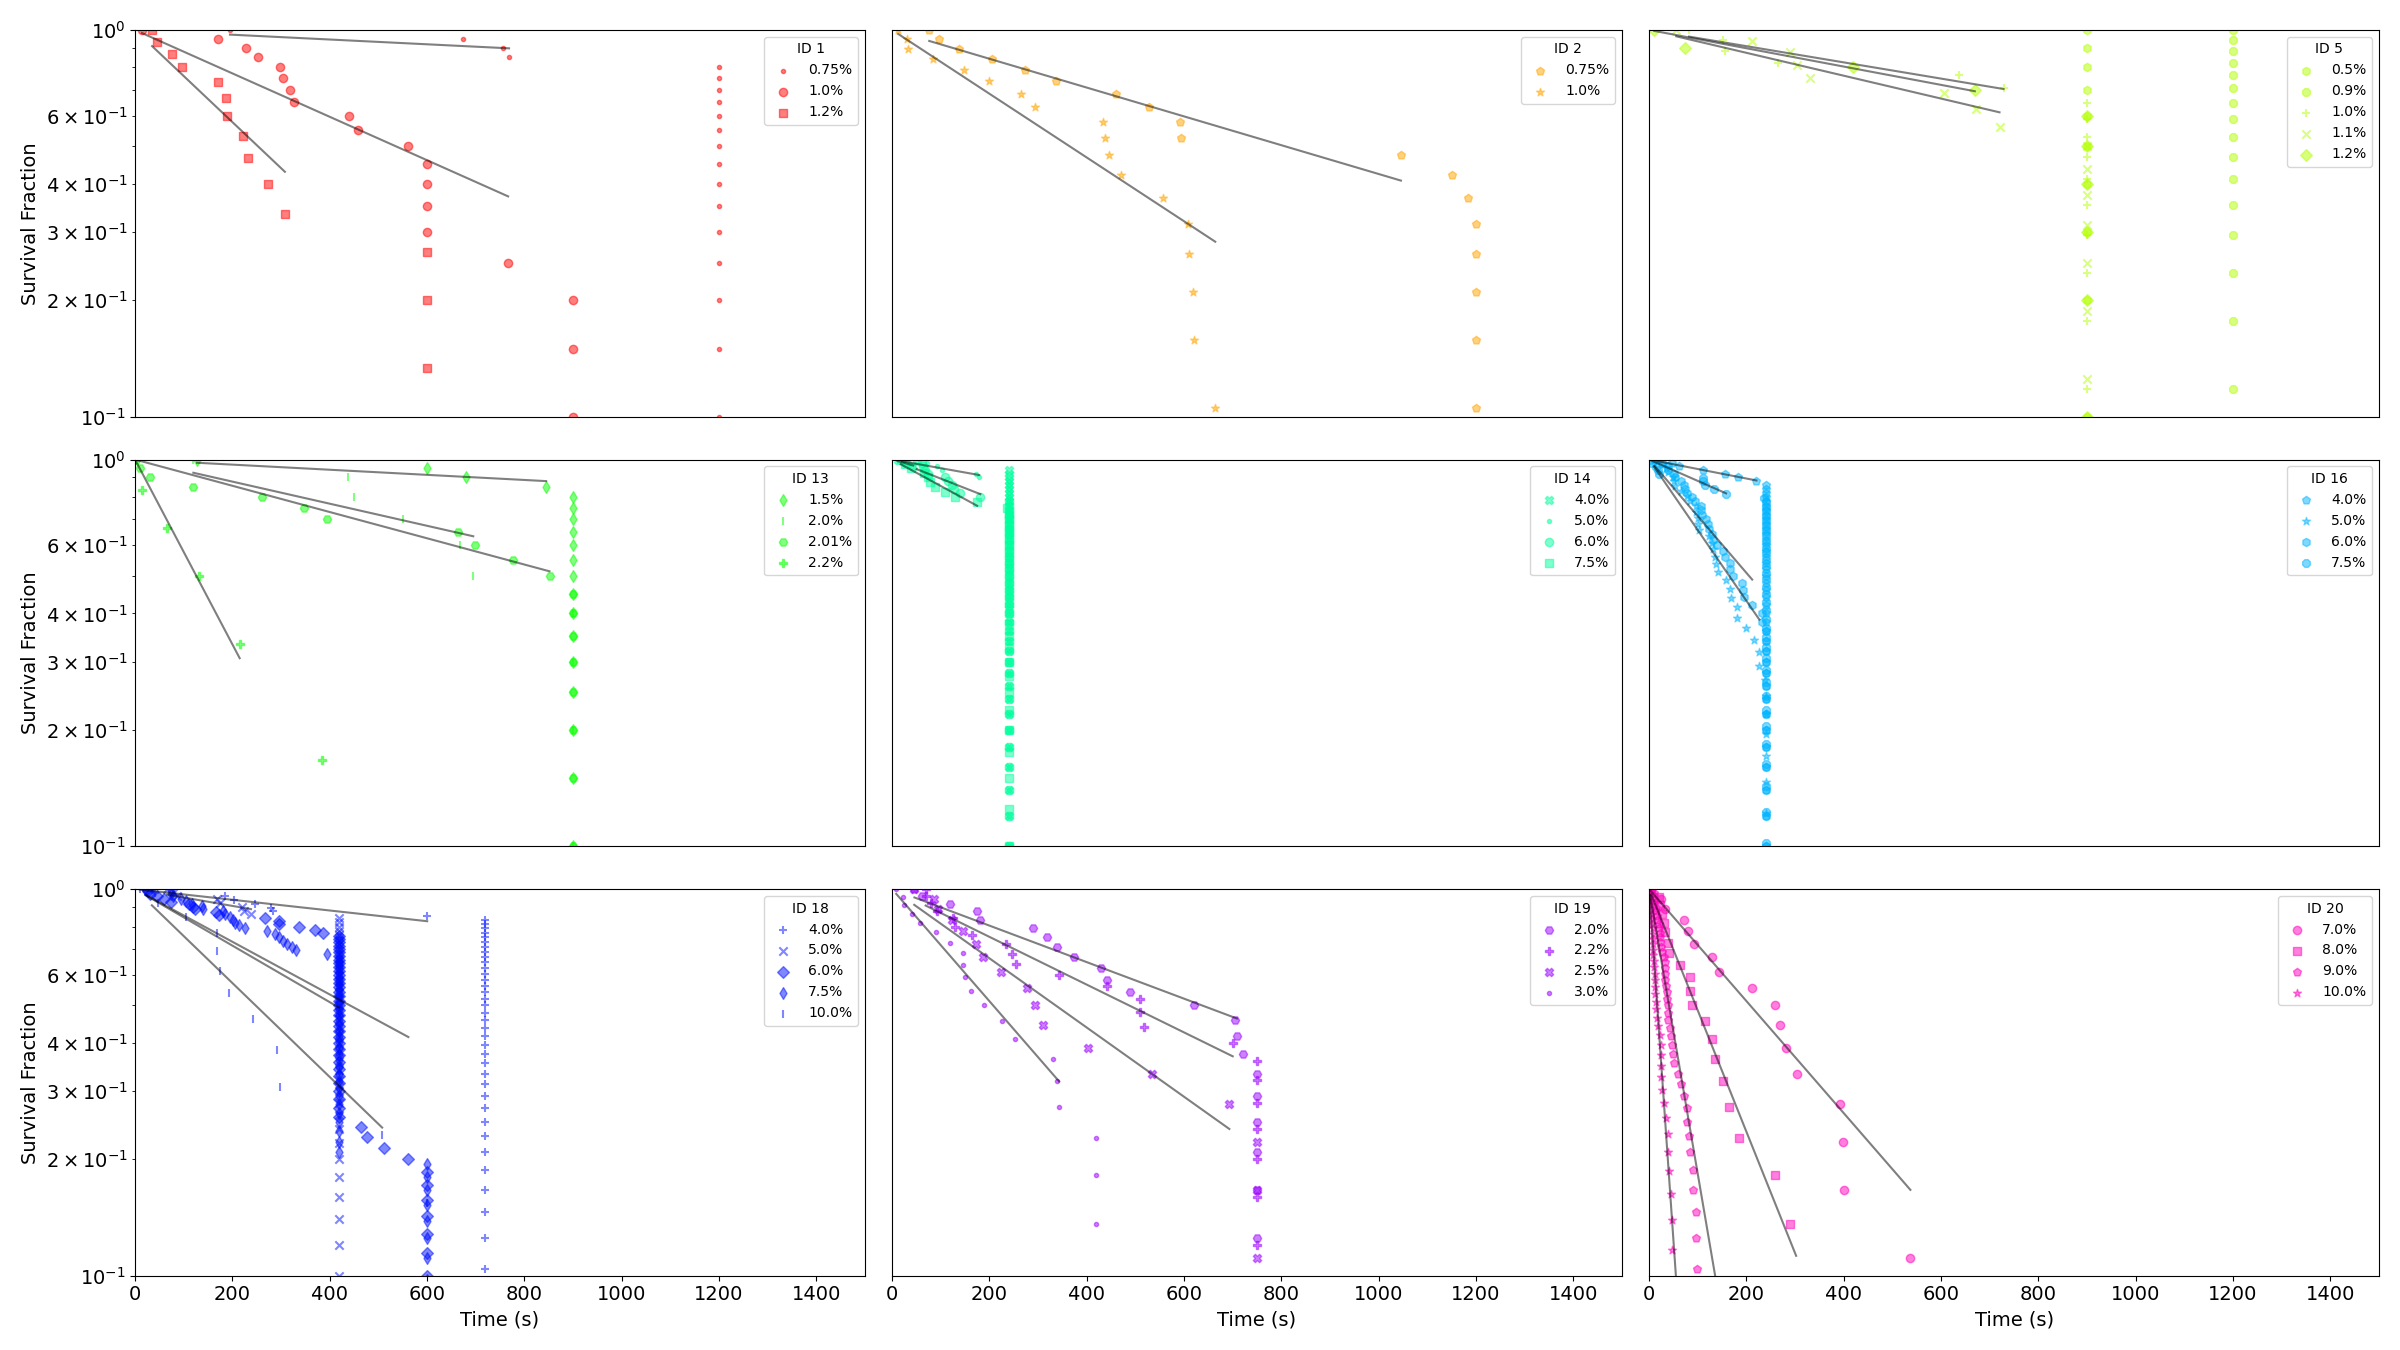
\includegraphics[width=1\linewidth]{Figures/multisurvival2Bis_Nef.png}}
	\caption{Survival of Nef-Nef19 bonds for 9 complexes and various applied acoustic power.}
	\label{fig:MultiSurvival_Nef}	
\end{figure}

\begin{figure}[hbt!]
	\centering
	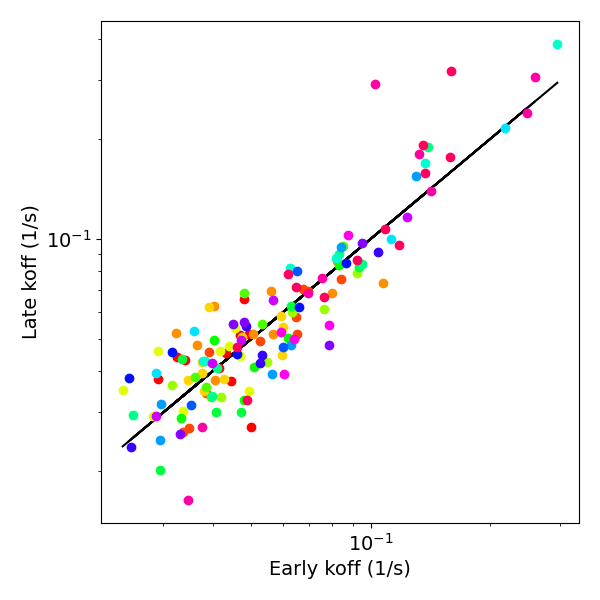
\includegraphics[width=0.4\linewidth]{Figures/Maturation_Rapa.png}
	\caption{Unbinding kinetics of FKBP12-Rapamycin-FRB bonds is not affected by repetitive force application and unbinding. The off-rate is calculated for each molecule and applied force based on the lifetime of the 50 first unbinding events (early koff) or 50 last unbinding events (late koff). }
	\label{fig:maturation}
\end{figure}


%\begin{figure}[hbt!]
%	\centering
%	\centerline {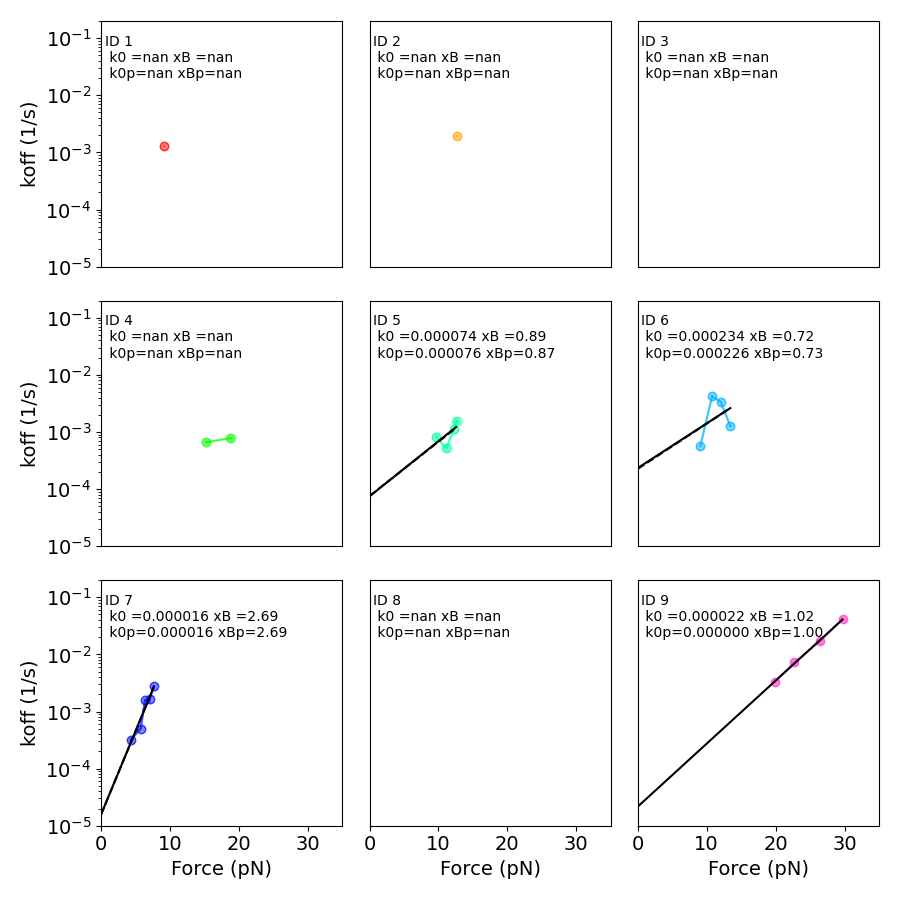
\includegraphics[width=1.2\linewidth]{Figures/offrate_vs_forceBis_Nef.png}}
%	\caption{Dependence of off-rate of Nef-Nef19 bonds as a function of force for 9 molecules (plain symbols). Plain line indicates fit with the Bell equation. Empty symbols are calculated using the force projected along the main axis of the scaffold, using the angle $\theta$.}
%	\label{fig:offrate_force_Nef}	
%\end{figure}




%\begin{table}[htbp]
%	\caption{Published kinetic parameters for the FKBP12-rapamycin-FRB  FKBP12-rapamycin  FRB reaction.  corresponds to the dissociation equilibrium constant,  to the dissociation rate constant, and  to the association rate constant. a}
%	\begin{tabular}{|l|c|c|c|c|c|c|c|}
%		\hline
%		Assay & Monitoring technique & Buffer b &  ($^{\circ}$C) c &  (nM) &  (10-3 s-1) d &  (106 M-1 s-1) & Reference \\ \hline
%		Titration by FRB
%		of GST-FKBP12•rapamycin
%		immobilized on anti-GST surfaces e & Surface plasmon resonance & PBS pH 7.4
%		50 nM rapamycin & 25 & 12 $\pm$ 0.8
%		11 $\pm$ 0.0 & 22
%		19 & 1.92
%		1.70 & Banaszynski et al. 2005
%		[18] \\ \hline
%		Titration by FRB
%		of GST-FKBP12•rapamycin
%		immobilized on anti-GST surfaces & Surface plasmon resonance & PBS
%		50 nM rapamycin & NS & 19 $\pm$ 0.5 & 16.7 $\pm$ 0.3 & 0.90 $\pm$ 0.01 & Flaxman et al. 2019 [19] \\ \hline
%		Force spectroscopy (Bell analysis)
%		with FRB and FKBP12•rapamycin
%		engrafted on a J-DNA scaffold e,f & Single-molecule assay
%		on a MT setup
%		(force cycling mode) & 20 mM HEPES pH 7.8
%		100 mM KCl, 5 mM MgCl2
%		500 nM rapamycin & 21.7 &  & 29.0 $\pm$ 0.6
%		29.6 $\pm$ 1.2
%		30.8 $\pm$ 0.3 &  & Kostrz et al. 2019 
%		[1] \\ \hline
%		Force spectroscopy (Bell analysis)
%		with SNAP-FRB and
%		CLIP-FKBP12 •rapamycin
%		engrafted on a J-DNA scaffold f & Single-molecule assay
%		on a MT setup
%		(force cycling mode) & 20 mM HEPES pH 7.8
%		100 mM KCl, 5 mM MgCl2
%		500 nM rapamycin & 21.7 &  & 31.7 $\pm$ 0.9 &  & Kostrz et al. 2019
%		[1] \\ \hline
%		Titration by rapamycin
%		of FRB and FKBP12
%		engrafted on a J-DNA scaffold & Single-molecule assay
%		on a MT setup
%		(force clamping mode) & 20 mM HEPES pH 7.8
%		100 mM KCl, 5 mM MgCl2
%		0.05 to 500 nM rapamycin & 21.7 &  & 35 &  & Kostrz et al. 2019
%		[1] \\ \hline
%		Force spectroscopy (Bell analysis)
%		with FRB-FH1-FKBP12•rapamycin
%		mounted on I27 and DNA handles g & Single-molecule assay
%		on a MT setup
%		(force cycling mode) & PBS
%		10 nM rapamycin & NS &  & 26 &  & Wang et al. 2019
%		[20] \\ \hline
%		Titration by FKBP12•rapamycin
%		of FRB-FH1-FKBP12•rapamycin
%		mounted on I27 and DNA handles h & Single-molecule assay
%		on a MT setup
%		(force cycling mode) & PBS
%		100 nM rapamycin & NS & 3.3; 8.5 & 32; 82 & 9.6 $\pm$ 1.2 & Wang et al. 2019
%		[20] \\ \hline
%		Force spectroscopy (Bell analysis)
%		with FRB and FKBP12•rapamycin
%		engrafted on a J-DNA scaffold f & Single-molecule assay
%		on an AFS setup
%		(force cycling mode) & 20 mM HEPES pH 7.8
%		100 mM KCl, 5 mM MgCl2
%		500 nM rapamycin & 25 &  & 26 $\pm$ 2 &  & Wang et al. 2022
%		(this study)  \\ \hline
%	\end{tabular}
%	\label{}
%\end{table}

\end{document}
